% !TEX TS-program = xelatex
% !TeX program = xelatex
% !TEX encoding = UTF-8
% !TEX spellcheck = en-US

\documentclass{aak-thesis}


%======================================================
\DeclareMathOperator{\ssfgc}{\textit{SSF-GC}}
\DeclareMathOperator{\ord}{\textit{ord}}
\DeclareMathOperator{\iord}{\textit{iord}}
\DeclareMathOperator{\simil}{\textit{sim}}
\DeclareMathOperator{\nextsent}{\textit{next}}
\DeclareMathOperator{\lastsent}{\textit{last}}
\DeclareMathOperator{\tfisf}{\textit{tf-isf}}
\DeclareMathOperator{\tfidf}{\textit{tf-idf}}
%======================================================

\hypersetup{
	pdfauthor={Abdelkrime Aries},
	pdftitle={Vers une amélioration du résumé auomatique de textes},
	pdfkeywords={Summarization; Multilingual},
	pdfsubject={Computer science; Artificial intelligence; Natural language processing}
}

%======================================================

\DeclareAcronym{ats}{
	short = ATS ,
	long  = Automatic text summarization ,
	class = abbrev
}

\DeclareAcronym{svd}{
	short = SVD ,
	long  = Singular value decomposition ,
	class = abbrev
}

\DeclareAcronym{lsa}{
	short = LSA ,
	long  = Latent semantic analysis ,
	class = abbrev
}


\DeclareAcronym{rts}{
	short = RTS ,
	long  = Real-Time Summarization ,
	class = abbrev
}

\DeclareAcronym{mms}{
	short = MMS ,
	long  = Multilingual Multi-document Summarization ,
	class = abbrev
}


\DeclareAcronym{mss}{
	short = MSS ,
	long  = Multilingual Single document Summarization ,
	class = abbrev
}

\DeclareAcronym{onforums}{
	short = OnForumS ,
	long  = Online Forum Summarization ,
	class = abbrev
}


\DeclareAcronym{cccs}{
	short = CCCS ,
	long  = Call Center Conversation Summarization ,
	class = abbrev
}

\DeclareAcronym{tcc}{
	short = TCC ,
	long  = Topic Clustering and Classification ,
	class = abbrev
}

\DeclareAcronym{be}{
	short = BE ,
	long  = Basic Element ,
	class = abbrev
}


\DeclareAcronym{autosummeng}{
	short = AutoSummENG ,
	long  = AUTOmatic SUMMary Evaluation based on N-gram Graphs ,
	class = abbrev
}

\DeclareAcronym{memog}{
	short = MeMoG ,
	long  = Merged Model Graph ,
	class = abbrev
}

\DeclareAcronym{npower}{
	short = NPowER ,
	long  = N-gram graph Powered Evaluation via Regression ,
	class = abbrev
}


\DeclareAcronym{tac}{
	short = TAC ,
	long  = Text Analysis Conference ,
	class = abbrev
}


\DeclareAcronym{ntcir}{
	short = NTCIR ,
	long  = NII Testbeds and community for Information access Research ,
	class = abbrev
}

\DeclareAcronym{ssf-gc}{
	short = SSF-GC ,
	long  = Sentence statistical features - Graph-based cumulative score ,
	class = abbrev
}


\DeclareAcronym{trec}{
	short = TREC ,
	long  = Text REtrieval Conference ,
	class = abbrev
}

\DeclareAcronym{hlda}{
	short = hLDA ,
	long  = hierarchical Latent Dirichlet Allocation topic ,
	class = abbrev
}

\DeclareAcronym{nist}{
	short = NIST ,
	long  = National Institute of Standards and Technology ,
	class = abbrev
}

\DeclareAcronym{ir}{
	short = IR ,
	long  = Information retrieval ,
	class = abbrev
}

\DeclareAcronym{api}{
	short = API ,
	long  = Application programming interface ,
	class = abbrev
}

\DeclareAcronym{rouge}{
	short = ROUGE ,
	long  = Recall-Oriented Understudy for Gisting Evaluation ,
	class = abbrev
}

\DeclareAcronym{bleu}{
	short = BLEU ,
	long  = BiLingual Evaluation Understudy ,
	class = abbrev
}

\DeclareAcronym{scu}{
	short = SCU ,
	long  = Summary Content Unit ,
	class = abbrev
}

\DeclareAcronym{nlp}{
	short = NLP ,
	long  = Natural Language Processing ,
	class = abbrev
}

\DeclareAcronym{lstm}{
	short = LSTM ,
	long  = Long Short-Term Memory ,
	class = abbrev
}

\DeclareAcronym{relu}{
	short = ReLU ,
	long  = Rectified Linear Unit ,
	class = abbrev
}

\DeclareAcronym{mse}{
	short = MSE ,
	long  = Mean Square Error ,
	class = abbrev
}

\DeclareAcronym{ml}{
	short = ML ,
	long  = Machine Learning ,
	class = abbrev
}

\DeclareAcronym{mmr}{
	short = MMR ,
	long  = Maximal Marginal Relevance ,
	class = abbrev
}


\DeclareAcronym{ar}{
	short = AR ,
	long  = Anaphora Resolution ,
	class = abbrev
}

\DeclareAcronym{tf}{
	short = TF ,
	long  = Term Frequency ,
	class = abbrev
}

\DeclareAcronym{idf}{
	short = IDF ,
	long  = Inverse Document Frequency ,
	class = abbrev
}

\DeclareAcronym{tfidf}{
	short = TF-IDF ,
	long  = Term Frequency-Inverse Document Frequency ,
	class = abbrev
}

\DeclareAcronym{tfisf}{
	short = TF-ISF ,
	long  = Term Frequency-Inverse Sentence Frequency ,
	class = abbrev
}


\DeclareAcronym{html}{
	short = HTML ,
	long  = Hypertext Markup Language ,
	class = abbrev
}

\DeclareAcronym{see}{
	short = SEE ,
	long  = Summary Evaluation Environment ,
	class = abbrev
}


\DeclareAcronym{svm}{
	short = SVM ,
	long  = Support Vector Machine ,
	class = abbrev
}


\DeclareAcronym{rst}{
	short = RST ,
	long  = Rhetorical structure theory ,
	class = abbrev
}


\DeclareAcronym{ctm}{
	short = CTM ,
	long  = Contextual Topic Model ,
	class = abbrev
}

\DeclareAcronym{ttm}{
	short = TTM ,
	long  = Two-tiered Topic Model ,
	class = abbrev
}

\DeclareAcronym{rl}{
	short = RL ,
	long  = Reinforcement Learning ,
	class = abbrev
}

\DeclareAcronym{td}{
	short = TD ,
	long  = Temporal Difference ,
	class = abbrev
}

\DeclareAcronym{sarsa}{
	short = SARSA ,
	long  = State-Action-Reward-State-Action ,
	class = abbrev
}


\DeclareAcronym{nn}{
	short = NN ,
	long  = Neural Networks ,
	class = abbrev
}


\DeclareAcronym{r2n2}{
	short = R2N2 ,
	long  = Recurrent Reconstruction Neural Network ,
	class = abbrev
}


\DeclareAcronym{ae}{
	short = AE ,
	long  = Auto-Encoder ,
	class = abbrev
}

\DeclareAcronym{duc}{
	short = DUC ,
	long  = Document Understanding Conference ,
	class = abbrev
}

\DeclareAcronym{pcfg}{
	short = PCFG ,
	long  = Probabilistic Context Free Grammar ,
	class = abbrev
}

\DeclareAcronym{hmm}{
	short = HMM ,
	long  = Hidden Markov Model ,
	class = abbrev
}

\DeclareAcronym{dl}{
	short = DL ,
	long  = Deep Learning ,
	class = abbrev
}


%\usepackage[helvetica]{quotchap}

%======================================================
%\bibliographystyle{plainnat}
\bibliographystyle{abbrvnat}
%\bibliographystyle{humannat}
%\bibliographystyle{unsrtnat}
%\bibliographystyle{kindersc2}
%\bibliographystyle{dinat}

\begin{document}

% the front matter

\pdfbookmark{Cover page}{coverpage}
% some details about the thesis
\title{Vers une amélioration des résumés automatiques de textes}
\subtitle{Towards improving automatic text summaries}
%\subtitle{Towards ameliorating automatic text summarization}
\author{ARIES Abdelkrime}
%\setadvisor{Djamal-eddine Zegour}{Pr.}{ESI}
%\setcoadvisor{Walid Khaled Hidouci}{Pr.}{ESI}

% about the degree
%\degree{Doctor of Philosophy}
%
%\degreeyear{2018}
%\degreemonth{Month}

%\setheader{%
%	\begin{tabular}{ll}
%		\multirow{2}{*}{
\includegraphics[height=1.5cm]{figures/logo/ESI.png}} 
%		& R\'epublique Alg\'erienne d\'emocratique et populaire \\
%		& Minist\`{e}re de l'enseignement sup\'erieur et de la recherche scientifique\\
%		& \'Ecole nationale Sup\'erieure d'Informatique (ESI ex. INI)\\
%	\end{tabular}
%}
%
%\setfooter{%
%	\begin{tabular}{ll}
%		\multirow{2}{*}{
\includegraphics[height=1.5cm]{figures/logo/K-LCSI.png}} & \\
%		& Laboratoire de Conception  \\
%		& des Syst\`emes Informatiques \\
%	\end{tabular}
%}

\pagestyle{empty}
\newgeometry{left=3cm,right=2cm,top=1cm,bottom=1cm}

\noindent

\includegraphics[width=\textwidth]{figures/logo/esi-header.png}


\makeatletter % changes the catcode of @ to 11

\begin{center}
	
	{\Large \bfseries TH\`ESE}\\
	pour le grade de\\
	{\Large \bfseries DOCTEUR DE L'ESI}\\
%	Option: Informatique répartie et mobile (IRM)\\
	Option: Informatique\\
	{\bfseries École doctorale STIC}\\
	présentée par\\
	{\LARGE \bfseries \@author}\\[0.5cm]
	préparée au sein du laboratoire LCSI - ESI \\
	soutenue le 28 octobre 2020 à Alger\\[1cm]
	
	
	{\Huge \bfseries \@title}

	{\LARGE \slshape ``\@subtitle"}\\[1cm]
	
	Encadrée par : \textbf{Pr. ZEGOUR Djamel Eddine}
	
	Co-encadrée par : \textbf{Pr. HIDOUCI Walid Khaled}
\end{center}
\makeatother % changes the catcode of @ back to 12


\vfill

\noindent
\textbf{Composition du jury :}

\noindent
\begin{tabular}{p{.4\textwidth}p{.1\textwidth}p{.15\textwidth}p{.25\textwidth}}
	M. BALLA Amar & Prof & ESI & Président \\
	Mme BENATCHBA Karima & Prof & ESI & Examinatrice \\
	M. GUESSOUM Aberezzak & Prof & Univ. Blida & Examinateur\\
	M. FOUDIL Cherif & Prof & Univ. Biskra & Examinateur \\
	M. ZEGOUR Djamel Eddine & Prof & ESI & Directeur de thèse \\            
	
\end{tabular}

\vfill                  

\noindent\hrulefill\vskip 2pt

{ \renewcommand{\arraystretch}{0.6}
\noindent
\begin{tabular}{lll}
	\multirow{4}{*}{
\includegraphics[width=2.4cm,align=t]{figures/logo/K-LCSI.png}} &&\\
	&& \textbf{L}aboratoire de la \\
	&& \textbf{C}ommunication dans les \\
	&& \textbf{S}ystèmes \\
	&& \textbf{I}nformatiques \\
\end{tabular}
}

%\begin{center}
%	
\includegraphics[width=2cm]{figures/logo/K-LCSI.png}
%	Laboratoire de la communication dans les systèmes informatiques
%\end{center}



\restoregeometry
\cleardoublepage

%\maketitle
%\copyrightpage
\frontmatter
\pdfbookmark{Acknowledgment}{acknowledgment}
\chapter*{Acknowledgment}

\noindent
Foremost, I would like to express my sincere gratitude to my advisers Prof. Zegour and Prof. Hidouci for the continuous support of my Ph.D study and research, for their patience and guidance.\\[.25cm]

\noindent
Besides my advisers, I would like to thank the rest of my thesis committee for accepting to examine my humble work.\\[.25cm]

\noindent
My sincere thanks goes to every person who contributed to this work directly or indirectly.\\[.25cm]

\noindent
Last but not the least, I would like to thank my family for their support.


\pdfbookmark{Dedication}{dedication}
% dedication text
\chapter*{}

\vspace*{\fill}

\begin{flushright}
	\begin{minipage}[]{7cm}
	To my parents, brothers and sisters, friends, teachers and professors, students, colleagues, and all those who marked my life.\\[.1cm]
	
	To anyone working hard to improve others' lives.\\[.1cm]
	
	To myself for being able to defeat my perfection problem and complete this thesis in an imperfect way. 
\end{minipage}
\end{flushright}



\pdfbookmark{Abstract}{abstract}

\chapter*{Abstract}

%Context: data growth and need for summarization
%Nowadays, a great mass of information is generated constantly, which resulted in enhancing information availability. 
%Even so, accessing this information tend to be difficult due to redundancy and search time. 
%One way to improve information access is to use automatic text summarization (ATS).  
%A generated summary must be informative, readable and not redundant; Hence, automatizing this task can be challenging. 
%
% 
%In this thesis, we investigate different methods and approaches for ATS. 
%Due to the growth of multilingual content on the web, we are more interested in discussing these methods and approaches in a multilingual context. 
%To this end, we present summarization approaches using a taxonomy based on the nature of used resources.
%We discuss different evaluation methods and campaigns, as well, in hope to affording more insights about ATS. 
%
%% Proposed methods (TCC)
%We are interested in improving ATS especially in a multilingual context.
%Our intention is to insure the following conditions: simple adaptation, informative summaries and coherence. 
%We improved our previous method, called ``Topic clustering and classification" (TCC), to handle many languages.
%The method clusters different sentences; it learns how to classify these clusters; then, it scores each sentence based on its capacity to represent all these clusters. 
%We participated in MultiLing'15 workshop using TCC, which will be considered as a baseline in our new method. 
%
%% Proposed methods (SSF-GC)
%TCC uses statistical features to score sentences; but, how about the relations between these sentences?
%Our new method, called ``Sentence statistical features - Graph-based cumulative score" (SSF-GC), scores sentences using statistical features, then it uses a graph structure to enhance these scores. 
%The graph is not just used for scoring, but also to select candidate sentences (deleting noisy sentences).
%In addition, we propose some methods to extract sentences after scoring.
%SSF-GC affords good results and it was be able to surpass TCC in many languages. 
%
%% Proposed methods (ML2ExtraSum)
%As additional experiment, we propose a model based on neural networks for multilingual summarization. 
%To this end, we prepared a corpus by extracting different features from MultiLing'15 MSS corpus. 
%The proposed method learns how to score each sentence based on different features, how to cluster a document's language, and how to combine all features scores into one in order to estimate ROUGE-1 score.
%Unfortunately, this method was not able to defeat TCC in many languages. 
%Nevertheless, it gives some insights into future improvements.

Nowadays, a great mass of information is generated constantly.
With time, it is become more difficult to manage such information due to redundancy, multilingualism and search time.
In this thesis, we are interested on multilingual\footnote{multilingual system/method: which supports more than one language.} automatic text summarization (ATS). 
To this end, we start by regrouping ATS methods using a taxonomy based on the nature\footnote{Nature of used resources : if the used resources (programs and data) are specific to a given language, in addition to processing power.} of used resources.
Then, using this taxonomy, we choose which methods can better serve our objectives: a system simple to adapt which generates informative and coherent summaries.
We improved our previous method, called ``Topic clustering and classification" (TCC), to handle many languages.
This method has participated in MultiLing'15 workshop, and is considered as a baseline in this thesis. 
In our new method, called ``Sentence statistical features - Graph-based cumulative score" (SSF-GC), sentences are not just scored using statistical features, but also graph structure to enhance these scores. 
The graph is also used to filter unimportant sentences ; those having week links to others.
In addition, we propose some methods to extract sentences after scoring. 
This method affords good results and it was be able to surpass TCC in many languages. 
Finally, we tried to use surface features with neural networks to learn sentences scoring as a ROUGE-1 score regression. 
Unfortunately, this method was not able to defeat TCC in many languages. 
Nevertheless, it gives some insights into future improvements.

\chapter*{Résumé}

% Contexte: croissance des données et besoin de synthèse
%De nos jours, une grande masse d'informations est générée sans cesse; ce qui a permis d'améliorer la disponibilité des informations au grand publique.
%Toutefois, accéder à cette information a tendance d'être difficile en raison de la redondance et du temps de recherche.
%Un moyen d'améliorer l'accès à l'information consiste à utiliser le résumé automatique de textes (RAT).
%Un résumé doit être informatif, lisible et non redondant. 
%Par conséquent, automatiser cette tâche peut être difficile.
%
%%
%Dans cette thèse, nous étudions des différentes méthodes et approches pour le RAT.
%En raison de la croissance du contenu multilingue sur le Web, nous sommes davantage intéressés à discuter ces méthodes et approches dans un contexte multilingue.
%À cette fin, nous présentons des approches de résumé en utilisant une taxonomie basée sur la nature des ressources utilisées.
%Nous discutons également de différentes méthodes et campagnes d'évaluation dans l'espoir de fournir des informations supplémentaires sur le RAT.
%
%% Méthodes proposées (TCC)
%Nous sommes intéressés par l'amélioration de RAT, en particulier dans un contexte multilingue.
%Notre intention est d'assurer les conditions suivantes: adaptation simple, résumés informatifs et cohérence.
%Nous avons amélioré notre méthode précédente, appelée ``Topic clustering and classification" (TCC), afin qu'elle supporte plusieurs langues.
%La méthode regroupe les différentes phrases; elle apprend à classer ces groupes; ensuite, elle note chaque phrase en fonction de sa capacité à représenter toutes ces groupes.
%Nous avons participé à l'atelier MultiLing'15 en utilisant le TCC, qui sera considéré comme une base de référence dans notre nouvelle méthode.
%
%% Méthodes proposées (SSF-GC)
%TCC utilise des caractéristiques statistiques pour noter les phrases; mais, qu'en est-il des relations entre ces phrases?
%Notre nouvelle méthode, appelée ``Sentence statistical features - Graph-based cumulative score" (SSF-GC), permet de noter les phrases à l'aide de caractéristiques statistiques, puis elle utilise un graph pour améliorer ces scores.
%Le graph ne sert pas uniquement à la notation, mais également à la sélection de phrases candidates (suppression de phrases bruyantes).
%De plus, nous proposons quelques méthodes pour extraire les phrases après la notation.
%SSF-GC donne de bons résultats et a pu dépasser TCC dans de nombreuses langues.
%
%% Méthodes proposées (ML2ExtraSum)
%Comme expérience supplémentaire, nous proposons un modèle basé sur les réseaux de neurones pour le résumé multilingue.
%À cette fin, nous avons préparé un corpus en extrayant différentes caractéristiques du corpus MultiLing'15 MSS.
%La méthode proposée apprend à noter chaque phrase en fonction de différentes caractéristiques, à regrouper la langue d'un document et à combiner toutes les notes des caractéristiques en une seule afin d'estimer le score ROUGE-1.
%Malheureusement, cette méthode n'a pas pu vaincre TCC dans de nombreuses langues.
%Néanmoins, elle donne un aperçu sur les améliorations futures.

De nos jours, une grande masse d'informations est générée sans cesse.
Avec le temps, il est devenu difficile de gérer une telle masse à cause de la redondance, multilinguisme et le temps de recherche.
Dans cette thèse, nous nous somme d'avantage intéressé par le résumé automatique de textes (RAT) dans un contexte multilingue\footnote{Système/méthode multilingue : qui peut supporter plus d'une langue.}.
À cette fin, nous commençons par regrouper les méthode de RAT en utilisant une taxonomie basée sur la nature des ressources\footnote{Nature des ressources : si les ressources (programmes et données) utilisées sont liées à une langue donnée. En plus, le coût en terme de puissance de calcul.} utilisées.
Ensuite, en utilisant cette taxonomie, nous avons choisi les méthodes qui peuvent mieux servir nos objectifs : un système simple à adapter qui génère des résumés informatifs et cohérents.
Nous avons amélioré notre méthode précédente, appelée ``Topic clustering and classification" (TCC), afin qu'elle supporte plusieurs langues.
Cette méthode a participé à l'atelier MultiLing'15, et elle est considérée comme une base de référence dans cette thèse.
Dans notre nouvelle méthode, appelée ``Sentence statistical features - Graph-based cumulative score" (SSF-GC), les phrases ne sont pas notées seulement à l'aide des caractéristiques statistiques, mais aussi à l'aide d'un graphe qui améliore ces scores.
Le graphe est aussi utilisé pour filtrer les phrases non importantes ; celles qui ont des relations faibles avec les autres. 
De plus, nous proposons quelques méthodes pour extraire les phrases après la notation.
Cette méthode donne de bons résultats et a pu dépasser TCC dans de nombreuses langues.
Enfin, nous avons essayé d'utiliser les caractéristiques de surface avec les réseaux de neurones afin d'apprendre la notation des phrase sous forme d'une régression sur le score ROUGE-1.
Malheureusement, cette méthode n'a pas pu vaincre TCC dans de nombreuses langues.
Néanmoins, elle donne un aperçu sur les améliorations futures.


\chapter*{\textarab{ملخّص}}

%
%\begin{arab}
%%السياق: نمو البيانات والحاجة إلى تلخيص
%في الوقت الحاضر، كمّيّة كبيرة من المعلومات يتمّ إنشاؤها باستمرار، مما أدى إلى تعزيز توافر المعلومات.
%رغم ذلك، الوصول إلى هذه المعلومات يمثّل صعوبة كبيرة بسبب التكرار ووقت البحث.
%واحدة من الطرق لتحسين الوصول إلى المعلومات هي استخدام التلخيص التلقائي للنصوص.
%الملخص الذي يتمّ إنشاؤه يجب أن يكون شاملا ومقروءً ولا يحتوي على التكرار؛ وبالتالي، فإنّ التلخيص التلقائي للنصوص يمكن أن تكون مهمّة صعبة.
%
%
%في هذه الأطروحة، نقوم بدراسة بعض الطرق والمناهج المختلفة للتلخيص التلقائي للنصوص .
%نظرًا لتنامي المحتوى متعدد اللغات على الويب، نحن أكثر اهتماما بمناقشة هذه الطرق والأساليب في سياق متعدد اللغات.
%لهذا السبب، سنعرض طرق التلخيص التلقائي مستخدمين في ذلك تصنيفا يعتمد على طبيعة الموارد المستخدمة.
%بالإضافة إلى ذلك، سنناقش  بعض أساليب وحملات تقييم الملخّصات على أمل تقديم مزيد من المعلومات حول هذا الموضوع.
%
%% الطرق المقترحة (TCC)
%نحن مهتمون بتحسين التلخيص التلقائي للنصوص خاصة في سياق متعدد اللغات.
%هدفنا هو تأمين الشروط التالية: سهولة تعديل النظام ليتكيّف مع لغة جديدة وغنى الملخّص بالمعلومات والترابط المنطقي للجمل.
%لذا فقد قمنا بتحسين طريقتنا السابقة، والتي تسمى \textLR{``Topic clustering and classification" (TCC) }، لتتعامل مع العديد من اللغات.
%طريقة \textLR{TCC} تقوم  بتقسيم الجمل إلى مجموعات .  بعدها،  تتعلّم كيفية تصنيف هذه المجموعات. ثم  تقوم  بتنقيط كلّ جملة بناءً على قدرتها على تمثيل كل هذه المجموعات.
%شاركنا في ورشة العمل \textLR{MultiLing'15} باستخدام \textLR{TCC} ، والتي ستعتبر خط أساس في طريقتنا الجديدة.
%
%%الطرق المقترحة (SSF-GC)
%تستخدم  \textLR{TCC} ميزات إحصائية لتنقيط الجمل؛ لكن، ماذا عن العلاقات بين هذه الجمل؟
%طريقتنا الجديدة، المسماة \textLR{ ``Sentence statistical features - Graph-based cumulative score" (SSF-GC)} ، تقوم بتنقيط الجمل باستخدام بعض الميزات الإحصائية، ثم تستخدم بنية المبيان لتعزيز هذه الدرجات.
%لا يتم استخدام المبيان للتنقيط فقط، ولكن أيضًا لاختيار الجمل المرشحة لتكون في الملخّص (حذف الجمل عديمة الجدوي).
%بالإضافة إلى ذلك ، نقترح بعض الطرق لاستخراج الجمل بعد تنقيطها.
%توفر  \textLR{SSF-GC} نتائج جيدة، حيث كانت قادرة على تجاوز  \textLR{TCC} في عدّة لغات.
%
%%الطرق المقترحة (ML2ExtraSum)
%كتجربة إضافية، نقترح نموذجًا يعتمد على الشبكات العصبية للتّلخيص متعدّد اللّغات.
%تحقيقًا لهذه الغاية، قمنا بإعداد مكنز من خلال استخراج ميزات مختلفة من مكنز \textLR{MultiLing'15 MSS}.
%تتعلم الطريقة المقترحة كيفية تنقيط  كل ّ جملة استنادًا على ميزات مختلفة .
%تتعلم أيضا على  كيفية إسناد كل نص إلى لغته.
%في الأخير، تقوم بدمج كل علامات الميزات في واحدة لتقدير درجة \textLR{ROUGE-1}.
%لسوء الحظ، لم تتمكن هذه الطريقة من هزيمة  \textLR{TCC}  في عدّة لغات.
%ومع ذلك، فإن هذه الطريقة تعطي بعض الأفكار حول التحسينات المستقبلية.
%\end{arab}

\begin{arab}
	في الوقت الحاضر، كمّيّة كبيرة من المعلومات يتمّ إنشاؤها باستمرار.
	مع الوقت، أصبحت معالجة هذه المعلومات صعبة جدا بسبب التكرار وتعدد اللغات ووقت البحث.
	في هذه الأطروحة، نحن مهتمون بالتلخيص التلقائي للنصوص في السياق متعدد اللغات\footnote{\textarab{طريقة أو نظام متعدد اللغات: يدعم أكثر من لغة واحدة.}}.
لهذا السبب، قمنا بتصنيف طرق التلخيص التلقائي معتمدين على طبيعة الموارد المستخدمة\footnote{\textarab{طبيعة الموارد المستخدمة: إذا كانت الموارد المستخدمة (البرامج والبيانات) خاصة بلغة معينة ، بالإضافة إلى قوة المعالجة.}}.
باستعمال هذا التصنيف، اخترنا الطرق التي بوسعها تأمين الشروط التالية: نظام سهل التعديل قادر على استخراج ملخصات غنية بالمعلومات ومتماسكة لغوبا.
قمنا بتحسين طريقتنا السابقة، والتي تسمى \textLR{``Topic clustering and classification" (TCC) }، لتتعامل مع العديد من اللغات.
هذه الطريقة شاركت في ورشة العمل \textLR{MultiLing'15} ، وستعتبر خط أساس في هذه الأطروحة.
أما في طريقتنا الجديدة، المسماة \textLR{ ``Sentence statistical features - Graph-based cumulative score" (SSF-GC)} ، فالجمل لا تنقط باستخدام بعض الميزات الإحصائية فحسب، وإنماياستخدام بنية المبيان لتعزيز درجاتها.
المبيان يستخدم أيضا لحذف الجمل عديمة الجدوي؛ تلك التي لديها روابط ضعيفة مع الأخريات.
بالإضافة إلى ذلك ، نقترح بعض الطرق لاستخراج الجمل بعد تنقيطها.
توفر  هذه الطريقةنتائج جيدة، حيث كانت قادرة على تجاوز  \textLR{TCC} في عدّة لغات.
في الأخير، جاولنا استخدام بعض الميزات السطحية مع الشبكات العصبية لتقدير درجة \textLR{ROUGE-1}.
لسوء الحظ، لم تتمكن هذه الطريقة من هزيمة  \textLR{TCC}  في عدّة لغات.
ومع ذلك، فإن هذه الطريقة تعطي بعض الأفكار حول التحسينات المستقبلية.
\end{arab}



\chapter*{Automatic summary}

We will express these extraction methods based on: the next sentence to be added to the summary ($ \nextsent $), a function affording the sentence which maximize/minimize a score ($ \arg\max $/$ \arg\min $), the score using a variant of our scoring method ($\ssfgc(s_i) $), similarity between two sentences ($ \simil $ ), the last sentence added to the summary ($ \lastsent $), and the descending/ascending order ($ \ord $/ $ \iord $) based on a given score.
Using some features of a sentence and its document, the system must learn to estimate ROUGE-1 of this sentence based on a reference summary.
During summary generation, a system must exclude similar sentences even if they score more than others.
So, the next sentence to be added to the summary using this method ($\nextsent_{e1}$) is the one ($s_i$) having the highest score ($ \ssfgc $) among candidate sentences minus those already in the summary ($ C\backslash S $).
So, the next sentence to be added to the summary using this method ($\nextsent_{e0}$) is the one having the highest score ($ \ssfgc $) among candidate sentences minus those already in the summary ($ C\backslash S $).
So in summary, the method wants to learn how to estimate ROUGE-1 score of a sentence using some surface features.
To extract a summary based on sentences scores, we used two extraction methods: the plain one based on the scores order and the one proposed in based on sentences similarities.
First sentences summarizer takes the first sentences of each document as a summary.
An extraction method is introduced based on sentences similarities and their scores in order to minimizing redundancy in the summary.\footnote{The English Abstract is 1976 characters long and this automatic one is almost the same size. To extract this summary, we used GC1 scoring method with e4 extraction method. Most of sentences came from GC chapter, but we can see some from ML2ExtraSum chapter. This is because we fuse the chapters all together in their original order. Also, we get rid of the titles and all \LaTeX commands such as figures, tables, equations, etc.}


\cleardoublepage
\pdfbookmark{\contentsname}{toc}
\renewcommand{\baselinestretch}{1} 
\setcounter{tocdepth}{1}
\tableofcontents
%\authorlist
\listoffigures
\listoftables
\listabbreviations
%\dedicationpage
%\acknowledgments
%
%\onehalfspacing
%\settocdepth{section}
\newpage
\mainmatter
\renewcommand{\baselinestretch}{1.5} 

% include each chapter...

\begin{savequote}[75mm] 
The world is one big data problem.
\qauthor{Andrew McAfee} 
\end{savequote}

\chapter{Introduction}

%problem of huge data
%\lettrine[lraise=0.1, nindent=0em, slope=-.5em]{W}{e}
We
live in the age of data, where a huge mass of information is produced everyday. 
It can be found in many sources, such as electronic newspapers, with many variations.
The redundant information makes their selection and processing very difficult.
One way to ease this task is using automatic text summarization. 

%Summary benefits
A summary, as defined in TheFreeDictionary\footnote{TheFreeDictionary: \url{http://www.thefreedictionary.com/outline} [February 07, 2017]}, is ``\textit{a brief statement that presents the main points in a concise form}".
One of its benefits is identifying the content of a given document, which will help readers picking the right documents of their interests.
According to \citet{75-borko-bernier}, a summary has many benefits such as saving time, easing selection and search, improving indexing efficiency, etc. 
Summaries of the same document can be different from person to person. 
This can occur due to different points of interest or due to each individual's understanding.

%History
\ac{ats} is not a new field of research. 
Since the work of \citet{58-luhn}, many works have been conducted to improve this field of research. 
Since then, despite the huge amount of researches conducted in this field, it still suffers from many challenges. 
In this introductory chapter, we will present some challenges facing \ac{ats}.
We will present this thesis motivation and aims, finishing by a discussion and outline of the next chapters.



\section{Summarization challenges}

There exists a lot of challenges which harden the advance of \ac{ats}. 
One of these problems is the absence of a precise definition of what should be included in a summary. 
Over time, several works were conducted to generate the perfect summary which must be informative on one hand, and not redundant on the other. 
%The first challenge is the definition of a good summary, or more precisely how can a summary be generated. 
Our needs for a summary are good indicators of what it should be: extractive or abstractive, generic or query-driven, etc. 
Even if we get the idea how humans usually summarize, implementing it will not be easy. 
Designing a powerful automatic text summarizer needs a lot of resources either tools or corpora. 
Another type of challenges is the summary informativeness; How can a system imitate human beings in summarizing task?
The coherence of the summary is one of the challenges that stood for years. 
Mostly, \ac{ats} methods aim to generate an informative summary, but when it comes to the summary's readability it is a matter of future work.  

\subsection{Definition}

A good summary can be defined as the shortest and more informative grammatically correct one without redundancy. 
This definition seems simple, but when we want to implement such idea, we will come across a lot of choices. 
A text, usually, contains a main topic and some satellite topics. 
For instance, if we talk about PCs, we may also include some commercial notions to express the market shares.
The choice of what topic to favor raises the question: what is a good summary?
If the summarization system is query-based, it is settled that the most similar the topics are to the request the more they are relevant. 
Nevertheless, Some may argue that adding relevancy to the main topic along with the request can be helpful for some users.

When it comes to generic summarization systems, it is more difficult to decide what is better for the reader.
Some researches try to capture the most relevant sentences from each topic to form a summary \citep{11-song-al}. 
The summary can cover all topics of a text, but sometimes it got far from the main point.
%
Others select only most relevant sentences to the main topic and ignore secondary ones. 
This leads to a summary that focuses on the main topic, and ignores the others which can be as important as the main topic.
%
Sure we have to give more importance to the main topics, but the satellite ones count too. 
This is what some researches are trying to achieve; a balance between the main topic and other topics that may contain some useful information \citep{12-zhang-al,13-aries-al}. 
For instance, in our previous work \citep{13-aries-al}, we try to regroup the sentences in different topics using a cosine similarity based clustering algorithm. 
A sentence can belong to more than one topic. 
Then, we use some statistical features with Naive-Bayes learning algorithm to model each topic to, finally, score each sentence according to its capacity of representing all these topics. 
This can give each topic a chance to participate in scoring sentences.


\subsection{Summary informativeness}

The main goal of a summary is to afford a representative text of the original document. 
It must cover the essential information using few words. 
That means, the summary must retain more information with less redundancy. %retain vs. maintain

\subsubsection{Summary coverage}

A summary must cover the most important content of the original document. 
When we read a summary, we must get an idea on what its original document is about, or what the document can tell us about a specific request. 
Information quantity has been the main target of evaluation methods, and workshops as well. 
A lot of advance has been made in this direction; so it may be considered as a minor problem compared to others.
For example, in MultiLing 2015, the systems had recall scores close to the top-line system which is a system that cheats while generating summaries.
That being said, a summary's coverage is an issue when it comes to generic systems which are not specific to any domain and language.  


\subsubsection{Summary conciseness}

A good summary must not contain redundant information; leaving the space for more useful information to be included. 
Most systems reorder sentences using their scores and extract the highest scored ones to form a summary.
But, sometimes, two similar sentences can be included into the summary especially in case of multi-document summarization.
During summary generation, a system must exclude similar sentences even if they score more than others.
A very known work that takes redundancy in consideration is \ac{mmr} \citep{98-carbonell-goldstein}.
The authors score each candidate sentence $ s_i $ of a document $ D $ (which is not already included into the summary $ S $) using two scoring similarities: $ \text{\textit{sim}}_1 $ which calculates the similarity of $ s_i $ to a query $ Q $, and $ \text{\textit{sim}}_2 $ which calculates the similarity of $ s_i $ to another sentence $ s_j \in S $.
The idea is to maximize MMR score given in Equation \ref{eq:mmr}.
\begin{equation}
	\label{eq:mmr}
	MMR = \arg \max \limits_{s_i \in D\backslash S} [ \lambda\, \text{\textit{sim}}_1 (s_i, Q) - (1-\lambda) \max\limits_{s_j \in S} \text{\textit{sim}}_2 (s_i, s_j)]
\end{equation}
Where, $ \lambda $ is a parameter that balances between the relevance ($ \lambda = 1 $) and the diversity ($ \lambda = 0 $).
The authors use cosine similarity to calculate $ \text{\textit{sim}}_1 $ and $ \text{\textit{sim}}_2 $.
%

More complex methods have been proposed to find a trade-off between coverage and conciseness of the generated summary.
For instance, \citet{12-nishikawa-al} model text summarization as a knapsack problem to generate a summary with a maximum coverage, selecting sentences with as many information units (unigrams and bigrams) as possible.
Then, they add a constraint to prevent adding a unit that already exists in the summary.

The two previous methods try to score sentences based on their coverage and conciseness in the same time.
A more simpler method is to score sentences using just coverage then regulate redundancy while selecting summary ones.
In \citep{15-aries-al}, cosine similarity and a threshold are used to decide two sentences similarity. 
The most scored sentence is considered to be in the summary.
It is selected only if it is not similar to the last added one.

We must point out that redundancy is not just a property of texts; it can be found even in videos. 
\citet{16-bhaumik-al} divide a video into multiple shots from which key-frames are extracted. 
Then, they remove intra and inter-shots redundant frames to form the final video summary.


\subsection{Summary readability}

%Post-processing
Extractive summarization methods are based on extracting pertinent units (sentences often) from the source document(s). 
The extracted units are used to form a summary, which often leads to dangling anaphora references and sentences which are ordered badly.
Abstractive methods seem to handle the anaphora problem and the order of sentences, since the generation is from a semantic representation. 
But the problem is, can the generator afford a good grammar with a fluent language? 
Summary readability has been in ``future works" section for years, a future that has never come. 

\subsubsection{Reference clarity}

When we extract summaries, some references such as personal pronouns remain unsolved. 
That way, the reader cannot find out who or what is involved in the sentence.
So, to generate a good summary we have to replace the first reference in the summary. 
For instance, if we have a text ``Karim is writing a thesis. He is almost finishing it." and the second sentence is select as a summary, we must replace ``He" with ``Karim" and ``it" with ``the thesis" so the summary can be understandable.
In \citep{16-bayomi-al}, it is found that introducing \ac{ar} can slightly improve the readability of the summary. 
Also, the authors confirm that the impact of \ac{ar} varies from one domain to another which means it improves some domains summaries more than others.

The resulted summary's readability can be enhanced by resolving anaphora, but it can even improve the process of summarization itself. 
\citet{07-orasan-stafford} try to test the effect of \ac{ar} on the summarization process using \ac{tfidf} for scoring and three different \ac{ar} methods.
The informativeness of generated summaries improves when \ac{ar} is used before summarization. 
On the other hand, it has no correlation with the performance of the anaphora resolver used to improve frequency calculation. 
\citet{07-steinberger-al} incorporate \ac{ar} into a complex scoring method which improves its performance even with an imperfect anaphora resolver.
To improve the coherence, they propose an algorithm to replace incorrect anaphoric relations in the summary by their respective original expressions in the text, which leads to a precision of 69\%.


\subsubsection{Coherence}

Most summarization methods are based on extracting relevant sentences and present them as they are. 
It would be a good idea if these sentences are reordered since they are extracted from different parts of a text. 
When reading a summary, the reader has to feel some flow of ideas without just jumping from idea to another.

%Ordering in single document summarization
In single document summarization, it seems right to present them as ordered in the original text. 
That is, reordering them using their original positions \citep{99-mckeown-al,00-radev-al,02-lin-hovy}. 
But, sometimes it will be better to move a sentence towards another due to their similarities. 
Methods which use rhetorical relations, such as \citep{98-marcu}, do not suffer this problem since they keep the relations between sentences.
%ENHANCE more sentence ordering for signle document. summmarization

In multi-document summarization, sentence reordering is important since the sentences come from different sources. 
The main topic of these documents must be the same, but the secondary topics are not always the same in each document.
Moreover, sentences in each source document are not ordered in the same flow of ideas. 
Some works tried to solve this problem differently. 
One solution is ``Majority Ordering" \citep{02-barzilay-al}, where similar sentences are grouped together into themes. 
Then, a graph representing the local order is created, where each node represents a theme. 
Two nodes are connected with an arc if, in a document, one sentence of the first node's theme is followed by another of the second node's theme.
The weight of this arc is the number of documents where this order is observed.
To infer the global order of the graph, an approximation algorithm is used.
Other variations of this method can be found in the works of \citet{05-bollegala-al,08-ji-nie}.

\subsubsection{Grammaticality}

A sentence can be grammatically incorrect when being generated by an \ac{ats} system. 
In case of extractive summarization, a summary is mostly formed of complete sentences extracted from the original document. 
This means, as long as the sentences from the original text are correct as long the summary's will be. 
Extracting phrases to form a summary such in \citep{18-gehrmann-al} can be challenging in term of grammaticality. 
Abstractive summarization is more concerned by this challenge, since the text is generated from semantic representations or using \ac{ml} models. 

\subsection{Resources}

One of the most problematic challenges in \ac{ats} is the lack of resources. 
Nowadays, there are many powerful tools for stemming, parsing, etc. compared to the past. 
Nevertheless, there still exists the challenge of finding adequate ones for a certain problem of summarization. 
Besides, finding or creating annotated corpus for \ac{ats} can be seen as a challenge as well.
%In this section, we will try to present some freely available resources which can be helpful to researchers.

\subsubsection{Toolkits}

%Summarization toolkits
Generally, when we create a new method, we have to compare it to other existing methods.
We can generate summaries with these different methods including ours and evaluate them using the earlier presented evaluation metrics.
In the past, it was difficult to find existing methods' implementations, and if found they probably be costly.
So, we have to implement them ourselves or contact the paper's authors. 
This have been changed recently with the flourishing of open source mentality among academics as well as industrial companies. 

%preprocessing toolkits
Summarization methods can be hard to be implemented, especially when they are heavily based on complex \ac{nlp} functionality. 
\ac{nlp} methods are more advancing by time, such as tokenizers, stemmers, syntactic parsers, etc.
Unfortunately, many original systems used to test these methods are not available either openly or commercially. 
There are some languages that lack basic \ac{nlp} tools such as tokenizers and stemmers.
Recently, there seems to be a more interest on affording open source toolkits to support research among \ac{nlp} community.

\subsubsection{Corpora} 

%talk about training ressources (labled corpus, etc.).
Many research methods use machine learning to train the system on a labeled corpus and then test it on another one. 
The problem, in many cases, is the absence of adequate corpora for \ac{ats}. 
Text summarization task is affected by the genre of training corpus (news, novels, etc.), which imply the creation of diverse corpora based on the purpose of the system.
Some researches tried to create methods with semi-supervised learning to solve this problem \citep{02-amini-gallinari}.
%talk about testing corpus
%availability
To adjust this problem, some workshops like MultiLing propose tasks for summarization corpora creation. 
Also, they afford training and evaluation corpora for automatic text summarization.

\subsection{Evaluation}

%Evaluating ATS methods is still a challenging task. 
Comparing a generated summary automatically to some man-made summaries is good, but not enough. 
The summarization system still can generate a good summary which is not even close to the reference summaries. 
Also, using reference summaries is more likely to work with extractive systems better than abstractive ones. 
This is a brief summary of some challenges:
\begin{itemize}
	\item People write summaries differently, therefore we can not say this is the best summary for sure. 
	Hiring professionals to evaluate automatic summaries can be very expensive in term of coast and time. 
	Also, a summary can be judged differently from a person to another due to human variation.
	
	\item To face the problems with human evaluation, especially the evaluation time, automatic methods can be used. 
	Most automatic methods evaluate just the content without the quality aspect. 
	Also, they are more adequate for extractive summarization methods than the abstractive ones. 
	Using words or n-grams in a reference summary and comparing them to those of the automatic summary can favorize certain systems over other better ones. 
	%	If the reference summaries are created taking in mind the use the sentences of the original text with some changes, this can disfavor abstractive systems which generates totally new sentences. 
	%	In the contrary, if the reference summaries are using totally new words, the extractive summaries may be disadvantaged as well. 
	%	For that, no co-occurrence will be found between their words and those of the reference.
	
	\item Automating quality evaluation such as grammar, reference clarity and coherence can be very challenging. 
%	The challenge is the same as in \ac{ats} one, discussed earlier.
	It needs more profound linguistic analysis of the summary, with accurate and powerful tools.
	Also, the methods that can detect such flaws can be used to fix them in the first place.
	For example, if we can detect automatically that a sentence must come earlier than another, this can be added to the summarization systems to fix the problem.
	
\end{itemize}


\section{Thesis motivation}


Summaries can be very useful in real life applications.
For instance, they can enhance productivity and decision making in term of time.
Lets quote from \citep{02-mani-al}: ``Summaries as short as 17\% of full text length sped up decision-making by almost a factor of 2 with no statistically significant degradation in accuracy.".
It can save time, ease documents selection and improve indexing efficiency \citet{75-borko-bernier}.
Automatizing the generation of summaries can be beneficial in many cases. 
\citep{17-pashutan-al} investigated the impact of \ac{ats} on media Monitoring. 
They found out that even using a simple summarization system, employees workflow was greatly improved.
Moreover, it can improve other domains such as: medical domain \citep{05-afantenos-al,19-liang-al} and legal domain \citep{04-farzindar-lapalme,16-polsley-al}.

Recently, multilingual content started to grow considerably, which needs more adaptable methods for languages other than English.
As a result, multilingual text summarization began to receive more attention from research community. 
In 2011, TAC\footnote{TAC: Text Analysis Conference, \url{https://tac.nist.gov}} workshop included a task called ``MultiLing task", which aims to evaluate language-independent summarization algorithms on a variety of languages \citep{11-giannakopoulos-al}.
This task evolved in 2013 into a workshop called ``MultiLing workshop" as a community-driven initiative for testing and promoting multilingual summarization methods. 
%There were three tasks: ``Multi-document multilingual summarization" (MMS) \citep{13-giannakopoulos},  ``Multilingual single document summarization" (MSS) \citep{13-kubina-all} and ``Multilingual summary evaluation".
%Ten languages were used in MMS and forty in MSS task, and the evaluation was automatic using ROUGE-1, ROUGE-2 and MeMoG.
Afterwards, the workshop was held in 2015, 2017 and 2019. 
In the light of that, this thesis will present \ac{ats} with more focus on multilingual context.


\section{Thesis aims}

Motivated by the growth of multilingual content on the web, this thesis will be focused on multilingual \ac{ats}.
Multilingualism is the ability to use many languages in a specified task (in our case: \ac{ats}).
So, a multilingual method must be isolated from language's structure of the input text. 
By definition, most existing methods can be considered as language-independent. 
When it comes to implementing such method into a system, the general challenges presented earlier can be an issue:
\begin{itemize}
	\item Methods based on simple linguistic properties found in most/all languages such as proper nouns can be seen as language independent.
	However, when it comes to multilingual implementation, we face the problem of finding proper nouns for many languages. 
	\item Machine learning \ac{ats} methods can be language-independent.
	The language supported by the system depends on the resources used for its training. 
	The problem with this approach is its use of annotated corpora for each language we want to add. 
	
\end{itemize}

In conclusion, even if a method is language-independent, it can be difficult to adapting the system implementing it into new languages.
In this case, the system can be considered as partially language-independent. 
Our intention is to propose a new method that insures the following conditions:
\begin{itemize}
	\item Simple adaptation: 
	A good multilingual method is the one which can easily be adapted into as many languages as possible. 
	
	\item Informative summaries: 
	A generic method can afford less performance than a language-specific one. 
	So, for a generic method (system) to support many languages with a fair performance is a good method (system). 
	
	\item Coherence: In general, this task needs some language related information to be done properly. 
	In our case, we will focus on sentences ordering.
	
\end{itemize}


\section{Discussion and thesis Outline}

In this introductory chapter, we presented different summarization challenges. 
They are summarized into informativeness, readability, resources and evaluation. 
A summary must afford the most important ideas in the input document without repeating them; thus it has to be informative. 
A reader must be able to understand this summary; therefore, it must not contain dangling references, it must be coherent and most of all grammatically correct. 
To automatically generate such summaries, a system must use some resources either for preprocessing (eg. tokenizing and stemming), processing (eg. representing sentences as syntactic trees using parsers) or postprocessing (eg. anaphora resolution).
The availability of these tools for a given language is crucial for implementing such system. 
Resources are not just tools, they can be data as well which is used for training and testing the system. 
Speaking of testing, summary evaluation is another issue which we will discuss in this thesis with more detail due to its importance. 
Knowing all these challenges open opportunities to better design summarization methods.
Motivated by the exploding amount of multi-lingual data on the web, we focus more in this thesis on multi-lingual summarization.
A better summarization method in our view is the one providing good summaries with less resources either tools, data or computing power. 
When implemented, adjusting and applying the system on new languages must be easy.
The rest of this thesis is organized as follows.

Chapter 2 presents the different summarization methods following the taxonomy proposed by \citet{98-hovy-lin,99-sparckjones}. 
A summarization system can be categorized following the input text, the purpose or the output text. 
Based on the input text's properties (source size, specificity and form), a summarization system can be single document or multiple documents; domain-specific or general; or based on the text's form such as structures, scales, mediums and
genres. 
The purpose of the summarization categorizes a system into generic or query-oriented based the the audience; into indicative or informative based on the usage; into background or update based on expansiveness.
The output document (the summary) can be extractive or abstractive based on the derivation; Neutral or evaluative based on the partiality; Fixed or floating based on the conventionality. 
Some of these properties affect the capacity of multilingualism in a system. 
For instance, abstractive systems are very difficult to be adapted to new languages. 
In fact, we never happen to find an \ac{ats} abstractive system which does not use deep linguistic properties. 
As for the systems based on deep learning, they use words embedding to learn how to generate a text for a certain language. 
This will consume a very huge amount of information in order to learn, because the system does not just learn how to generate text but also it learns the vocabulary.  
Besides being an introduction into \ac{ats} domain, it will serve as a comparison between different methods in term of multilingualism.


After presenting different \ac{ats} methods, Chapter 3 categorizes them into approaches. 
Our taxonomy is based on the nature of resources used by the method (or the system) since we are more interested on multilingual summarization. 
So, the different approaches presented in this chapter are: statistical, graph-based, linguistic and machine learning. 
%Besides these approaches, we present sentence compression as an approach of \ac{ats} since it serves the same purpose and is mostly used by \ac{ats} systems to reduce sentences size.
Starting with statistical approach, we present the different surface features which exist since the beginnings of this domain. 
Despite being old, these features are still being used and gives good results especially in a multilingual context.
Another approach is graph-based, which represents the sentences as a graph of similarities to score each sentence and extract the most relevant ones.
In the contrary of these two approaches, the linguistic one is highly dependent on language.
It allows deep analysis of the input text leading to good results.
But, the system must target just one language at once.
Machine learning, on the other hand, can be considered as a statistical approach. 
The main difference between this approach and surface statistical features is that the former uses more resources in training. 


Discussing \ac{ats} methods and approaches cannot be complete without a quick dive into its evaluation.
This is why a glimpse into summarization evaluation methods and workshops is given in Chapter 4.
Evaluating summarization systems is one of the most difficult tasks.
As presented previously, one of summarization challenges is its definition: what is a good summary?
Evaluating a summary can defer from person to person and it can be subjective sometimes. 
So, many efforts have been affected in order to automatize evaluation or at least make it semi-automatic.
In addition, many workshops were organized to evaluating \ac{ats} systems.


Chapter 5 presents our participation in MultiLing'15 workshop in two tasks: single document and multi-documents summarization.
Our previous work \citep{15-aries-al} was enhanced and adapted to the context of multilingual summarization. 
The method clusters different sentences based on their cosine similarities and a given threshold. 
Each sentence can belong to many clusters which are considered as topics. 
Then, a Naive Bayes classifier is trained on these clusters using some features: term frequency (unigrams and bigrams), sentence position and length. 
The classifier is used as a scoring function to get which sentence can represent most topics. 
An extraction method is introduced based on sentences similarities and their scores in order to minimizing redundancy in the summary.


In chapter 6, we propose a new extractive method based on both surface statistical features and similarity graphs. 
First, a graph is constructed using similarities between sentences. 
Then, the graph is minimized by dropping weak sentences and links. 
The remaining sentences are considered as candidates for the summary. 
Each candidate sentence is scored using some surface features.
Then, the score is improved by the graph structure.
We propose four variants on how to improve the statistical score based on the graph. 
The final score is used to deciding which sentences are more informative than others.
The method's variants are tested against three baselines: random, first sentences and our previous method presented in Chapter 5.
Since informativeness is not the only issue with summarization, we propose some extraction methods that deals with other issues such as redundancy and sentences order.
These extraction methods are compared to our previous one proposed in \citep{15-aries-al}.
 


Finally, Chapter 7 concludes our work by summarizing our contributions, discussing the limits of our proposition and affording some insights into future works.
\begin{savequote}[75mm] 
By three methods we may learn wisdom: First, by reflection, which is noblest; Second, by imitation, which is easiest; and third by experience, which is the bitterest.
\qauthor{Confucius} 
\end{savequote}

\chapter{Summarization methods}
\label{chap:summeth}


Different summarization methods have been proposed since the first work of Luhn \citep{58-luhn}. 
Each method is intended to solve a problem in a certain context. 
A summarization system can be classified using many criteria; It can belong to many classes at once. 
These criteria are regrouped into three categories: input document criteria, purpose criteria and output document criteria \citep{98-hovy-lin,99-sparckjones}. 
Based on the criteria afforded by \citet{98-hovy-lin} and some other changes to fit current systems, the different classifications can be illustrated as in Figure~\ref{fig:summary-classif}.

\begin{figure}[ht]
	\begin{center}
		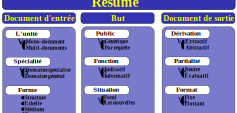
\includegraphics{figures/methods/sum-classif.pdf} % % %[width=140mm]
		\caption{Classification of summarization systems using different criteria.}
		\label{fig:summary-classif}
	\end{center}
\end{figure}

In this chapter, we will present each of these classifications in details with some examples. 
Each section will be reserved to one of the three classifications: input document, purpose and output document. 
Finally, we will discuss the impact of each method category on the multilingualism of the system (method).


\section{Input document focused summarization methods}

%======= Introduction ======= 
Examining the input document, a summarization system can be classified using three criteria: source size, specificity and form. 
Source size refers to how many documents a system can have as input. 
The specificity refers to the domains which this system can handle: is it designed just for a specific domain? or is it for general purpose? 
Input document(s) form specifies if they are structured or not, have low scale (tweets) or large one (novel), are textual or multimedia documents, and if they are of the same genre or not. 

%======= Source size ======= 
\subsection{Source size}

A summarization system can have one input document (single document) or many (multi-document) according to the source size criterion.
Some systems are designed to afford both single and multi-document summarization \citep{15-henss-al,15-aries-al}.
%definition
Single document systems process just one input document at once.
Even they use other documents for training, they still are using a single document as input. 
%works
This kind of summarization includes the first works of ATS \citep{58-luhn,58-baxendale,69-edmundson} as well as recent ones \citep{16-durrett-al,19-saini-al,19-liu-al}.
%benefit
It is simpler to process just one document since its sentences are more coherent and less redundant.
%limit
But, it is not adequate for all sort of applications.
For instance, if we want to summarize some news from different sources, we can end up with similar summaries if they talk about the same subject.

%definition
On the other hand, a multi-document system takes many documents of the same topic as input.
For example, summarizing news about a car crush from many newspapers. 
%works
The earliest work we can find in multi-document summarization is the work of \citet{95-mckeown-radev}. 
Some recent works focusing on this kind of summarization are \citep{15-zhong-al,19-tavir-al}.
%benefit 
The benefit of this type of summarization is to diversify information sources.
%limit
But, one of its most challenging issues is redundancy; documents talking about the same topic have much information in common.
%This classification (Single vs. Multi- document summarization) is very popular among researchers in the field of ATS. 


%======= Specificity ======= 
\subsection{Specificity}

An automatic summary can be generated from domain-specific documents or from general domains.
A domain is the general subject of a document; it can be high level such as sports, politics, science, etc. or low level such as football, tennis, etc. \citep{15-vander-al}.
%definition
Most works are not dedicated to a domain in particular even if they are tested on one. 
%works 
For instance, if someone uses cue words as in \citep{69-edmundson}, the method can be considered as domain-free (general) summarization. 
But, if these cue words are designed to favor some domain-related concepts such as medical domain \citep{09-sarkar}, in this case the method is domain specific. 
%benefits
In the end, general summarization systems can be beneficial since they can be applied to any domain. 
%limits
But, their performance will not be as good as domain-specific ones.


%definition
When we want to summarize documents of the same domain, it is more appropriate to use a summarization system specific to this domain. 
This can reduce terms ambiguities, the usage of grammar and formatting schemes. 
%works
Examples of domain-specific works: juridic texts \citep{04-farzindar-lapalme}, biomedical texts \citep{07-reeve-al}, medical texts \citep{09-sarkar,19-liang-al}.
%benefits
The performance of a domain-specific system should be better than a generic one, since it is designed for that matter.
%limits 
Designing such methods requires knowing the particularity of the domain so we can choose the right features.

%======= Form ======= 
\subsection{Form}

Input documents forms can be their structures, scales, mediums and genres. 
%definition
The structure refers to the explicit organization found in the document (eg. sections in papers: introduction, related works, method, experiments and conclusion).
The structure can be used to increase summarization performance where every section can be treated differently.
%works 
For instance, LetSumm system \citep{04-farzindar-lapalme} uses thematic structures in legal judgments (decision data, Introduction, Context, juridical analysis and Conclusion) to generate summaries. 
%For each thematic, some linguistic markers are affected to be used as cue phrases \citep{81-paice}. 
%The resulted summary is a combination of those thematic summaries with a percentage of contribution.
Another example is the work of \citet{07-pembe-gungor} who try to summarize \ac{html} documents. 
The sections are detected from \ac{html} tags to help reordering generated sentence
%benfits
Introducing document's structure helps summarization especially when users are more interested in a section than others. 
%limits
But, such methods can be applied to just the structures they are meant to work on.

%definition
The scale is another aspect which can affect the summarizing method; An input document can be a paragraph, an article, a book, etc. 
Many known summarization systems use term frequency as relevancy measure, therefore the input document must be large (important terms are repeated a lot).
%works
In case of summarizing low scale documents such as tweets \citet{10-sharifi-al,12-duan-al}, we cannot use usual techniques.
After all, a tweet is just as long as a summary itself. 
So, the summary is usually constructed from many tweets as input.
Some works limit the size of input document due to technical restrictions, such as using recurrent neural networks for abstractive summarization \citep{15-rush-al}. 
%benefits
Inventing new methods for different scales is a must when our documents have predefined sizes which can be as small as tweets or as large as encyclopedias.  
%limits 
These methods can face some challenges based on their specific scale.
If the document is too short, many known summarization techniques such as term frequency will not work on a single document.
If it is too large, processing time and memory can be an issue.

%definition
The medium is the support which carries the information.
Most summarization systems are based on textual support, while there are some researches on summarizing images, videos and audios.
%works
The work of \citet{14-gunhee-al} addresses the problem of jointly summarizing large-scale Flickr images and YouTube user videos. 
More works on multimedia summarization are: interactive football summarization \citep{09-moon}, summarizing important events in a football video \citep{12-zawbaa-al}, video summarization using web images \citep{13-khosla-al}, video summarization using a given category \citep{14-potapov-al}, video summarization by learning \citep{15-gygli-al,18-zho-al}.
%benefits 
Texts are not the only support that can benefit us when summarized; other supports such as multimedia content as abundant on the web as well.
%limits
These supports will not have the same methods as a text, and new methods must be adapted to each one.

%definition
Summarization systems can be classified using the genre of their input documents. 
A genre is defined as a complementary to domains covering non-topical text properties function, style,
and text type.  \citep{15-vander-al}.
As example, a document genres can be: news, interviews, reviews, novels, etc.
In this case, a method is created to support one genre, multiple genres or no genre at all (does not take genre in consideration).
%works
There are some works which adjust their scoring methods according to the document's genre.
The system is trained on multiple genres to select adequate features for each one \citep{07-goldstein-al} or to produce multiple summarization models for each genre \citep{10-yatsko-al}. 
Some systems are just designed for a specific genre, such as reviews \citep{09-zhan-al} and patents \citep{19-girthana-swamynathan}.
%benefits 
Specifying the genre of a method can be helpful especially when we are just interested in a very specific genre. 
%limits 
Though, it is not quit possible to defining a method for each genre. 


\section{Purpose focused summarization methods}

%======= Introduction ======= 
The purpose of summarization defines three criteria: audience, usage and expansiveness.
A summary audience specifies to whom it is intended: a specific user's profile or any user.  
The usage of summary can be helping users decide their interests or replacing the original document(s) as a shorter version of it.
As for the expansiveness, our definition is a little different from that of \citet{98-hovy-lin}. 
In our version, it is whether the summary have chronological knowledge of the past documents or not.

%======= Audience ======= 
\subsection{Audience}

Sometimes, users need a summary focusing on some aspects rather than the main idea of the input document. 
A summarization system which takes in consideration user's preferences is called query-oriented, while the one which does not is known as generic system. 
%definition
A generic summarization system tries to capture important information from an input document. 
So, we can say it tries to focus on the topic presented by the author and present what the input document is all about.
%works 
This type of systems exists widely, as an example: the systems in MultiLing'15 \citep{15-vanetik-litvak,15-aries-al,15-thomas-al,15-vicente-al}.
%benefits
This is beneficial if the readers are more interested in the main idea of a document.
%limits 
Nevertheless, sometimes readers are more interested in some subjects than others.

%definition
Query-oriented systems take in consideration users preferences.
For instance, if a user wants a summary focusing on someone in a story, it must contain events around this person without loosing the main interest of the story. 
%works
For instance, \citet{10-bhaskar-bandyopadhyay} describe a method to summarize multiple documents based on user queries.
The correlation measure between sentences from each document are calculated to create clusters of similar sentences.
Then, the sentences are scored according to the query.
This score is accumulated to the cluster score to extract the highest scored sentences.
Recent techniques such as deep learning have been used to generate query-oriented summaries \citep{15-zhong-al,19-kimuru-al}.
%benefilts
The benefit of query-oriented methods is clear: afford users with summaries based on their preferences.
%limits
The most challenging issue facing these methods is recovering query-relevant sentences of the documents that cover the main topics as well.

%======= Usage ======= 
\subsection{Usage}

A summary based on its usage is meant to help users decide their interests or as a representative replacement for the original document(s).
%definition
Informative summaries contain essential information of the original document(s); After reading them, you can tell what are the main ideas. 
This type of summaries can be found in journals, theses, research articles, etc. 
In a research article, the author must present the essential ideas and findings using an abstract which is considered as an informative summary.
%works
The majority of systems and methods focus on this type of summarization, hence we can find examples of this type anywhere.
%benefits
To sum up, Informative summaries are used as a short version of the input document(s).
%limits
Their main challenge is to express most ideas in the input document without redundancy.

Indicative summaries does not contain informative content; they only contain a global description of the original document. 
That includes the purpose, scope, and research methodology. 
This can be helpful to decide whether or not to consult the original document. 
The abstracts on the title page's verso of books and reports are an example of indicative summaries. 
Works have been conducted to investigate such type of summaries.
\citet{01-kan-al} propose an indicative multi-document summarization system (CENTRIFUSER) based on the problem of content planning. 
Figure \ref{fig:kan-al-exp} represents an example of a CENTRIFUSER summary on the health-care topic of ``Angina" where the generated indicative summary is in the bottom half using the difference in topic distribution of documents to regroup them.
%
\begin{figure}[ht]
	\begin{center}
		\includegraphics{figures/methods/kan-al-exp.pdf} % % %[width=140mm]
		\caption{An example of CENTRIFUSER summarizer output \citep{01-kan-al}.}
		\label{fig:kan-al-exp}
	\end{center}
\end{figure}
The method uses an IR system to search in a collection of documents, which gives a selected set of documents. 
Then some features are extracted from the collection and from the individual chosen documents to be used along with the query to generate the indicative summary.
%benefits
To sum up, Indicative summaries are used as a description to helping users select documents. 
%limits
Sometimes, it is more difficult to describe a document than finding out what it talks about. 
For instance, providing information about places (Where), persons (Who), etc. in a document.

%======= Expansiveness ======= 
\subsection{Expansiveness}

A generated summary can focus on original document's background, or afford the news compared to some past documents.
This property is referred to as expansiveness. 
A background summary, according to \citet{01-mani}, assumes that the reader has poor prior knowledge of general setting of the input text(s), and hence includes explanatory material, such as circumstances of place, time, and actors.
On the other hand, just-the-news summary is containing just novel or principal themes, assuming that the reader
knows enough background to interpret them in context. 
Nowadays, a lot of systems tend to afford the most relevant information found in input texts without verifying if the resulted summary incorporates some explanatory materials. 
Following the previous two definitions, these systems are neither background nor just-the-news. 
That is, such system can generate both background summaries and just-the-news ones. 
So, classifying systems based on whether or not they are designed to incorporate news is more appropriate.

%definition
Lets, first, redefine what just-the-news summaries and call them ``update summaries", since this term is more used. 
Recently, the emerging interest in systems that automatically monitor streams of social media posts such as Twitter or news to keep users up to date on topics they care about, led to the appearance of update summaries.
The idea is to generate summaries from some recent documents which do not contain information from previous documents. 
It means, the system must have prior knowledge of what has been seen before. 
%works
Update summaries were promoted in TAC 2008 as ``update task" \citep{08-dang-owczarzak} where the participants must generate multi-document update summaries from some chronologically ordered sets of news documents.
A more recent evaluation campaign for update summaries is ``Real-time summarization" task \citep{17-lin-al}.
%benefit
This type of summarization helps users to save time by reading just the news without consulting what they already know. 
%limits 
Besides the general challenges, update summarization must detect new information based on past documents. 
So, it has to take temporal information in consideration. 

%definition
We can, then, define a background summarization system as a system which generates summaries based on the input document(s) content and without excluding information from prior documents on the same subject. 
%works
Any system that does not have prior knowledge of past documents can be considered as a background summarization system. 
%benefits 
Compared to update summarization, this type can be used widely since it does not concern itself with documents chronological order.
%limits 
However, when this order is important to us, it is better to use update summarization over this one.

\section{Output document focused summarization methods}

Three criteria be used to classify a summarization system based on the summary: derivation, partiality and format.
Derivation means the fashion used to produce a summary from the original document, either by extracting relevant units or by creating a new text.
Partiality is how a summary handles the opinions found in the original document, which can be either neutral or evaluative.
As for format, the summary format can be fix or floating.

%===== Derivation ========
\subsection{Derivation}

It refers to the way used to obtain a summary. 
It can be by extracting pertinent units or by understanding and generating a new summary.
%definition
Extractive summaries are produced by, as the name says, extracting units from the original documents. 
Usually, these units are sentences because it is easy to keep the correctness of the summary's grammar.
%works
The first works in the field of \ac{ats} are extractive; they use some features to estimate the pertinence of a sentence.
Some of these features are: term frequency \citep{58-luhn}, position in the text \citep{58-baxendale,69-edmundson} and keywords \citep{69-edmundson}. 
Nowadays, this type of summarization is still widely applied \citep{17-ren-al,18-aries-al,19-liang-al}.
%benefits
What makes extractive methods so famous is their simplicity compared to the abstractive ones. 
They are simple to design, consuming less resources and giving good results.
%limits
However, they face many challenges such as informativeness and readability.

%information
Abstraction, on the other hand, is the generation of new text based on the input document(s).
Abstractive systems are difficult to design due to their heavy dependence on linguistic techniques.
Specifying the domain of a system can simplify the creation of this type of systems \citep{93-mitkov}.
%works 
The abstractive summary can be generated using a semantic representation of the text \citep{15-liu-al,19-barros-al,19-li-zhuge}.
Recently, many works try to generate abstractive summaries using deep learning \citep{15-rush-al,16-nallapati-al,17-ling-rush,19-you-al,19-shen-al}.
%benefits
Abstractive summaries are very important since they are similar to human abstracts. 
%limits
However, generating such summaries needs more resources in term of data, tools and processing time.

%===== Partiality ========
\subsection{Partiality}

Partiality, by definition, is the bias in favor of one thing over another. 
Following partiality criteria, a summarization system can be neutral or evaluative.
%Partiality~Neutral definition
A neutral system produces summaries which reflect the content of the input document(s) without judgment or evaluation. 
They are not designed to, specifically, include opinion into the summary even if the input document contains judgments.
%works
Most works fall into this class \citep{58-luhn,58-baxendale,69-edmundson,15-vanetik-litvak,15-aries-al,15-vicente-al,15-thomas-al,15-zhong-al}.
%benefits
The benefit of this type of methods is to present the general ideas in a document without trying to focus on opinions or giving some evaluations.
%limits
But, sometimes, some domains such as the juridical one needs more focus on evaluations than the main topic.

%Partiality~Evaluative definition
An evaluative system includes automatic judgments either implicitly or explicitly.
An explicit judgment can be seen as some statements of opinion included automatically.
The implicit one uses bias to include some material and omit another.
%works
A lot of examples can be afforded for this type of summarization, especially with the growth of interest towards users opinions. 
For instance, the work of \citet{16-othman-al} is based on summarizing customer opinions through Twitter. 
Given a conversation of tweets, the method tries to effectively extract the different product features as well as the polarity of the conversation messages.
The year 2008 knew the debut of a new task within TAC conference called ``Opinion Summarization task", which is meant to generate summaries from answers on opinion questions. 
%benefits
This kind of summarization can help us find opinions in reviews, legal judgments, etc.
It, also, allow us to generate summaries with some automatically generated opinions about a subject. 
%limits
Searching opinions in a document is not an easy task; it requires more knowledge of the type of documents. 

%======= Format ======
\subsection{Format}

Generated summaries must be presented using a format: as a list of sentences, as one paragraph, etc.
Some systems use a fixed format, while others present their summaries based on user preferences or based on some goals.
%definition 
A fixed format does not change from user to another or from summary purpose to another; it is always the same. 
%works
Most works fall into this class, since most of them are research systems which focus on the informational part of the summary rather than its format (presentation to the user).
%benefits 
Mostly, the generated summary is used to help users having a general idea about the documents; so, just one output format is enough.
%limits
However, with the variety of devices settings and users interests, this kind of summarization can be arguable.


%definition
Floating-situation summarization systems try to display the content of summaries using variable settings to a variety of readers for diverse purposes. 
%works
The ONTOSUM system \citep{05-bontcheva} is one of these systems; it uses device profile (e.g., mobile phone, Web browser) to adjust the summary formatting and length. 
Another similar work is given in \citep{18-chongtay-al} where the authors propose a responsive news summarization system for multiple mobile devices. 
%benefits 
This kind seeks to improving readability based on users settings and preferences.
%limits
To our knowledge, there are few works on floating situation summarization; all of them focus on responsive summary size.  


\section{Discussion}

% summarize the taxonomy
%========================
We presented different summarization categories based on the taxonomy found in \citep{98-hovy-lin,99-sparckjones}. 
%Our intention in this chapter is to present these methods and discuss their suitability for multilingual text summarization. 
%But before that, lets enlist the different categories. 
A method's categorization can be done based on three criteria: input document, purpose and output document. 
Looking to the input document, we can classify a method based on source size (multi-document, vs. mono-document), specificity (domain-specific vs. general) and form (structure, scale, medium and genre). 
The purpose of a summarization method contains three sub-criteria: audience (query-oriented vs. generic), usage (indicative vs. informative) and expansiveness (background vs. just-the-news).
We changed the definition of the last one (Expansiveness) to fit nowadays methods, this will categorize summaries into background or update.


% input document 
%=================
Lets start by assessing the impact of the input document categorization on multilingual text summarization. 
% source size
Source size has nothing to do with documents' languages. 
So, if a method is either multi-document or mono-document, this does not affect its multilingualism. 
Of course, if we want to go deep in processing multiple documents using their semantic relationships, in this case a multilingual method can be difficult to set in motion. 
% Specificity
Specificity criterion separates summarization methods into domain-specific and general. 
A domain-specific method uses language resources such as cue words to emphasize a domain over others, which makes it language-dependent. 
On the bright side, being dependent to a domain can help limiting the workload of adapting a certain system to a new language. 
For instance, it is fairly easy to prepare a list of domain words in a certain language, either manually or automatically. 
% form
Summarization systems based on document form are dependent to the structure, scale, medium and genre rather than the input language. 

% purpose
%==========
A summarization method can be categorized according to its purpose based on three criteria: audience, usage and expansiveness.
% Audience
According to the audience criterion a summary can be query-oriented or generic, both can be language independent.
In case of query-oriented methods, there is always a technique to consider users queries without relying on heavy language resources. 
For instance, cosine similarity can be used to calculate the pertinence of a sentence to the query based on their terms. 
% Usage
Looking to the summary's usage, a summary (and the method as well) can be indicative or informative.
An informative summary can be done without relying on heavy language resources. 
As for an indicative summary, if the purpose is to present a little text to invite the reader for reading the whole document, we can apply the  same analogy as informative one. 
If we want to present some information such as ``Who", ``When", ``Why", etc., in this case more language dependent resources are needed.
% Expansiveness
The expansiveness divides summaries into background and update summaries. 
Both of these categories can be generated without relying on heavy language resources.
For instance, in update summaries we can detect novelty using some statistical methods such as cosine similarity.

% Output document
%==========
A summarization method can be categorized according to its output document (the summary) based on three criteria: derivation, usage and expansiveness.
% Derivation
According to derivation, a summarization method can be extractive or abstractive.
The extractive one can rely only on statistical methods to extract some parts of the text, thus it can be language-independent. 
The abstractive, on the other hand, has to use some language information to generate new texts. 
Using Deep learning to produce new texts, the architecture itself is not designed for a specific language. 
But when it comes to the training set, we need a huge amount of text so the system learns a vocabulary and some generation rules. 
%This makes it so hard to adapt the system to many languages and 
% Partiality
According to partiality, a method (or a system) can be neutral or evaluative . 
The latter includes opinion, which can be implicit or explicit. 
Either ways, the system must rely on some language material to detect text opinions in case of implicit summarization, or to understand the text and generate opinions in case of explicit one. 
% Conventionality (Fixed, Floating)
The conventionality criterion, which divides methods into fixed or floating, has no relation with language. 



\begin{savequote}[75mm] 
By failing to prepare, you are preparing to fail.
\qauthor{Benjamin Franklin} 
\end{savequote}

\chapter{Summarization approaches}
\label{chap:app}


%TODO introduction 

In this chapter, we will discuss different approaches of \ac{ats}. 
According to \citet{12-nenkova-mckeown}, topic representation approach contains topic words, frequency driven, latent semantic analysis, etc. 
We are, rather, interested in the nature of used resources.
Are they dependent on a specific language? or domain? do the methods need a lot of resources?
This is why we follow their other taxonomy \citep{11-nenkova-mckeown} called ``Semantics and discourse" which we present as ``linguistic approach" since its methods as highly connected to the language being processed.
The taxonomy of \citet{12-lloret-palomar} seems to approach our vision. 
The difference is that we consider topic-based and discourse-based approaches as sub-approaches of linguistic one, since the two are based on linguistic properties of the input text.

\section{Statistical approach}

Statistical approach has been used in ATS since its first days. 
It is based on some features which are used to score the relevancy of text units (generally, sentences) to the main topic or users requests. 
%These features can be combined to score the units using many aspects, and get the highest scored ones.
Usually, to score a unit many statistical features are used as shown in equation \ref{eq:combin-crit}.
\begin{equation}
	\label{eq:combin-crit}
	Score(s_i) = \sum_{f \in F}{\alpha_f * Score_f(s_i)}
\end{equation}
Where $ \alpha_f $ is the weight of a feature $ f $ in the features set $ F $.
The features weights can be fixed manually or using machine learning techniques.
Also, other methods such as optimization can be used. 
For instance, \citep{17-feigenblat-al} propose an unsupervised query-focused multi-document summarization method based on Cross-Entropy (CE) method \citep{04-rubinstein-kroese}. 
It seeks to select a subset of sentences that maximizes a given quality target function using some statistical features.


\subsection{Term frequency (TF)}

\ac{tf} is the oldest feature \citep{58-luhn} and the most famous one. 
In his work, the terms frequency used to measure significant words, which has to be between two thresholds to ensure that the term is important yet not specific to the text's domain.
It supposes that frequently repeated terms in a text are important.
This feature is still being used in conjunction of machine learning, such as the work of \citet{17-yousefiAzar-hamey}.

\ac{tf} has a problem when it comes to domain-relative words; For example, in documents talking about computer science, certain words such as ``computer" will have great frequencies even if they do not represent the main topic.
To address this problem, \citet{58-luhn} uses two thresholds to ensure that the term is important yet not specific to the document's domain.
A more advanced solution is to use \ac{tfidf} which is first defined by \citet{73-salton-yang}.
Given a corpus $ D $ containing many documents $ d \in D $, the measure \ac{idf} is calculated as shown in Equation~\ref{eq:idf}.
\begin{equation}
	\label{eq:idf}
	idf(t) = log{\frac{|D|}{|\{d \in D /\ t \in d\}|+1}}
\end{equation}
Where: 
$ |D| $ is the number of documents in corpus $ D $;
$ |\{d \in D /\ t \in d\}| $ is the number of documents containing the term $ t $.

\subsection{Position in the text}

The position of words \citep{58-luhn} and sentences \citep{58-baxendale,69-edmundson} in a text has good potential of capturing their importance. 
In \citep{58-luhn}, the position of words in a sentence is used to create some sort of groups, where each one is the set of significant words separated by at most 5 to 6 non-significant words. 
Then, the group which has the most significant words is used to score the sentence, as shown in Figure \ref{fig:luhn-score}.

\begin{figure}[!ht]
	\centering
	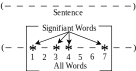
\includegraphics[width=50mm]{figures/approaches/luhn-score.pdf} % % %[width=140mm]
	\caption{Luhn score using word position \citep{58-luhn}.}
	\label{fig:luhn-score}
\end{figure}

The position of sentences in a text is used as indicator of its importance: the first and the last sentences tend to be more informative than the others \citep{69-edmundson}.
For instance, in scientific articles, sentences from the  introduction and the conclusion contain more information about the topic than other sentences.
In \citep{58-baxendale}, it is established that the first and the last sentences in paragraphs are more important. 
The author used a corpus of 200 paragraphs to test the importance of sentences according to their positions in a paragraph. 
He found out that in 85\% of these paragraphs, the first sentence is the most important; and that in 7\% of them the last one is.
Afterward, \citet{69-edmundson} formulated a hypothesis that sentences which appear very soon or late in the document or paragraphs have a good chance to be topic sentences.

Position feature can be used differently to score sentences.
\citet{04-nobata-sekine} define three methods to score a sentence $ s_i $, where $ i $ is its position in a document of $ n $ sentences.
The first method Equation (\ref{eq:nobota-pos-1}) supposes that only the first sentences less than a defined position $ N $ are important.
\begin{equation}
\label{eq:nobota-pos-1}
Score_{pos}(s_i) = \left\lbrace 
\begin{array}{lll}
1 & if & (i < N) \\
0 & otherwise & \\
\end{array}
\right. 
\end{equation}
The second method (Equation \ref{eq:nobota-pos-2}) supposes that a sentence's importance is inversely proportional to its position.
\begin{equation}
\label{eq:nobota-pos-2}
Score_{pos}(s_i) = \frac{1}{i}
\end{equation}
The last method (Equation \ref{eq:nobota-pos-3}) supposes that the first and the last sentences are more important.
\begin{equation}
\label{eq:nobota-pos-3}
Score_{pos}(s_i) = \max(\frac{1}{i}, \frac{1}{n-i+1})
\end{equation}
According to the authors, the second method gives the best results among the three.
%
\citet{09-abdelfattah-ren} use the position of sentences in paragraphs instead of the whole text. 
They suppose that the 5 first sentences in a paragraph are the most important (Equation \ref{eq:abdelfattah-pos}).
\begin{equation}
\label{eq:abdelfattah-pos}
Score_{pos}(s_i) = \left\lbrace 
\begin{array}{lll}
6 - i & if & (i \leq 5)\\
0 & otherwise &  \\
\end{array}
\right. 
\end{equation}
Where: $ i $ is the position of the sentence in the paragraph.

Like Luhn, \citet{10-ouyang-al} use word position based on the hypothesis that a word is more informative if it appears earlier in the text.
Therefore, the position of a word can be calculated according to its other occurrences in the whole text and not just according to other words in the sentence.
For that, four different functions are defined: Direct proportion (DP), Inverse proportion (IP), Geometric sequence (GS) and Binary function (BF). 
Direct proportion (DP) attributes a score of $ 1 $ of the first appearance and $ 1/n $ to the last one as, where $ n $ is the count of words in the sentence. 
Then the function to calculate DP is given in Equation \ref{eq:p_dp}, where $ i $ is the position of the word in the sentence. 
\begin{equation}
\label{eq:p_dp}
f_{DB}(i) = \frac{(n - i +1)}{n}
\end{equation}
Inverse proportion (IP) function is given in Equation \ref{eq:p_ip}, where the degree decreases quickly at smaller positions. This gives advantage to leading sentences. 
\begin{equation}
\label{eq:p_ip}
f_{DB}(i) = \frac{1}{i}
\end{equation}
Geometric sequence (GS) function scores an appearance of a word as the sum of the scores of all its following appearances (Equation \ref{eq:p_gs}).
\begin{equation}
\label{eq:p_gs}
f_{GS} (i) = (1/2)^{i-1}
\end{equation}
Binary function (BF) affords more importance to the first appearance of a word, and the others an equally less importance.
Therefore the first one will get a score of $ 1 $ and the others a score of a given $ \lambda \ll 1 $ as shown in Equation \ref{eq:p_bf}.
\begin{equation}
\label{eq:p_bf}
f_{BF} (i) = \left\lbrace 
\begin{array}{lll}
1 & if & i = 1\\
\lambda & otherwise &  \\
\end{array}
\right. 
\end{equation}
The final score is calculated as shown in Equation \ref{eq:ouyang-pos} 
\begin{equation}
\label{eq:ouyang-pos}
Score(s) = \sum\limits_{w_i \in s} \frac{\log(freq(w_i)) * pos(w_i)}{|s|} 
\end{equation}
Where $ pos(w_i) $ is one of the four functions shown previously; $ freq(w_i) $ is the frequency of the word $ w_i $; $ |s| $ is the length of the sentence.

\subsection{Title and subtitle words}

``The title carries the topic of the document", this hypothesis was first introduced by \citet{69-edmundson}.
When we divide a document into sections and subsections, we choose representative titles for each. 
So, any sentence containing some words of a title is considered as important.
This feature can be treated as if the title was a request \citep{88-salton-buckley}. 

\citet{01-ishikawa-al} fuse this feature with term frequency, in a way that the frequencies of the title words are weighted more than regular words.
In Equation \ref{eq:ishikawa-head}, a sentence $ s_i $ is scored by the frequencies of its words $ w $; if the word belongs to the title, its frequency is multiplied by a number $ A > 1 $ (the authors used $ A = 3 $).
%\begin{equation}
%\label{eq:ishikawa-head}
%Score_{title}(s_i) = \sum_{\{w\} \in s_i}{\alpha(w) * tf(w)}
%\end{equation}
%Where: 
%\[ 
%\alpha(w) = \left\lbrace 
%\begin{array}{lll}
%A > 1 & if & w \in title \\
%1 & otherwise & \\
%\end{array} 
%\right. 
%\]
\begin{equation}
	\label{eq:ishikawa-head}
	Score_{title}(s_i) = \sum_{\{w\} \in s_i}{\alpha(w) * tf(w)} 
	\text{ where }
	\alpha(w) = \left\lbrace 
	\begin{array}{ll}
		A > 1 & \text{if } w \in title \\
		1 & otherwise \\
	\end{array} 
	\right. 
\end{equation}
%%04-nobata-sekine
To score sentences based on title's words, \citet{04-nobata-sekine} propose two methods.
The first method uses $ tf*idf $ of the title's words $ T $ as indicated in Equation \ref{eq:nobta-head-1}.
\begin{equation}
\label{eq:nobta-head-1}
Score_{title}(s_i) = \frac{\sum_{w \in T \bigcap s_i}{\frac{tf(w)}{tf(w)+1} idf(w)}}
{\sum_{w \in T}{\frac{tf(w)}{tf(w)+1} idf(w)}}
\end{equation}
The second method uses named entities $ e $ and frequencies of words $ tf $ as shows in Equation \ref{eq:nobta-head-2}.
\begin{equation}
\label{eq:nobta-head-2}
Score_{title}(s_i) = \frac{\sum_{e \in T \bigcap s_i}{\frac{tf(e)}{tf(e)+1}}}
{\sum_{e \in T}{\frac{tf(e)}{tf(e)+1}}}
\end{equation}
According to the authors, the second method gives better results.

\subsection{Sentence length}

This feature was used to penalize too short sentences \citep{95-kupiec-al}.
Given a threshold, for example 5 words, the feature is true if it exceeds this threshold and false otherwise.
Sentences which are very small, in number of words, are unlikely to be important so it is better to omit them.
A more complex formula to score a sentence is expressed in the two methods proposed by \citet{04-nobata-sekine}.
The first method scores a sentence based on its length and a predefined maximum value $ L_{max} $ as shown in Equation \ref{eq:nobota-len-1}.
\begin{equation}
\label{eq:nobota-len-1}
Score_{length}(s_i) = \left\lbrace 
\begin{array}{lll}
\frac{|s_i|}{L_{max}} & if & (|s_i| \leq L_{max}) \\
1 & otherwise & \\
\end{array}
\right. 
\end{equation}
The second, which gives better results, affords a negative score to penalize sentences shorter than a predefined minimum value $ L_{min}$ (Equation \ref{eq:nobota-len-2}).
\begin{equation}
\label{eq:nobota-len-2}
Score_{length}(s_i) = \left\lbrace 
\begin{array}{lll}
0 & if & (|s_i| \geq L_{min}) \\
\frac{|s_i| - L_{min}}{L_{min}} & otherwise & \\
\end{array}
\right. 
\end{equation}
As observed by the authors, the second method is the best.

A more recent formula proposed by \citet{09-abdelfattah-ren} is indicated in Equation \ref{eq:abdelfattah-len}.
It scores a sentence $ s_i $ using its words number $ |s_i| $, the document's words number $ |d| $ and the number of sentences in this document $ |\{s: s \in d\}| $.
\begin{equation}
	\label{eq:abdelfattah-len}
	Score_{length}(s_i) = \frac{|s_i| * |\{s: s \in d\}|}{|d|}
\end{equation} 


\subsection{Centroid}

A centroid, as defined by \citet{04-radev-al}, is ``\textit{a set of words that are statistically important to a cluster of documents}". 
Since it is the most important in the cluster, the documents and sentences containing it are also important.
One famous summarization system using clusters centroid to extract summaries is MEAD \citep{00-radev-al,04-radev-al}.
MEAD is a multi-document summarizer, where similar documents to the centroid are clustered together.
Then, a set of parameters (Centroid value, Positional value, and First-sentence overlap) are used to rank each sentence from the resulting cluster.
The centroid value $ C_i $ for a sentence $ S_i $ is computed as in Equation \ref{eq:centroid}.
\begin{equation}
\label{eq:centroid}
C_i = \sum_{w \in S_i}  C_{w,i}
\end{equation}
Where, $ C_{w,i} $ is the centroid value of a word $ w $ in sentence $ S_i $.
The positional value $ P_i $ for a sentence $ S_i $ is computed according to its position in the document with $ n $ sentences as in Equation~\ref{eq:centroid-p}.
\begin{equation}
\label{eq:centroid-p}
P_i = \frac{n - i + 1}{n} * C_{max}
\end{equation}
Where $ C_{max} $ is the maximum centroid score in that document.
The First-sentence overlap value $ F_i $ of a sentence $ S_i $ is given as in Equation~\ref{eq:centroid-f}.
\begin{equation}
\label{eq:centroid-f}
F_i = \overrightarrow{S_1} \overrightarrow{S_i}
\end{equation}
Where $ S_1 $ is the first sentence.
These three scores are combined into one score along with a redundancy score to extract the most scored sentences.

A more recent work presents an unsupervised centroid-based document-level reconstruction framework using distributed bag of words model \citep{18-mani-al}.
The method uses machine learning to construct a distributed bag of words (DBOW) model for each document. 
Then, the centroid $ C $ of a multi-document set $ D = [d_1, d_2, ..., d_n] $ is given in Equation~\ref{eq:centroid-mani}.
\begin{equation}
\label{eq:centroid-mani}
C = \frac{1}{|D|}\sum\limits_{1}^{|D|} DBOW(d_i)
\end{equation}
The summary is constructed by iteratively selecting the sentences with the minimum reconstruction error (error between summary's DBOW and $ C $).

\subsection{Frequent itemsets}

Frequent itemsets are common sets of items which have at least a minimum amount of times. 
It was, first, proposed by \citet{94-agrawal-srikant} to solve the problem of discovering association rules
between items in a large database of sales transactions.
In ATS, the itemsets are considered as sets of terms extracted from sentences, where those which co-occur in many sentences are considered as frequent itemsets.

\citet{12-baralis-al} apply an entropy-based strategy to generate compact itemset-based models, where each document sentence is seen as a separate transaction. 
They formalize the problem of selecting sentences as a set covering optimization problem.
It is solved by a greedy strategy where sentences covering the maximum number of itemsets are selected.
This method is ameliorated in MWI-Sum system \citep{15-baralis-al} by replacing traditional itemsets with weighted ones in order to increase item relevance in the mining process. 
Also, \ac{tfidf} is used as relevance score. 

This approach is used in \citep{17-litvak-vanetik} with the minimum description length (MDL) principle that employs
Krimp compression algorithm \citep{11-vreeken-al} for query-based \ac{ats}.
The key idea is to use the query to select related frequent itemsets (word sets).
It is, also, combined with other approaches such as: Latent Semantic Analysis \citep{19-cagliero-al}, graphs \citep{18-azadani-al}, clustering \citep{19-rouane-al}, etc.

\subsection{Latent semantic analysis (LSA)}

\ac{lsa} seeks to analyze relationships between a set of documents and the terms they contain.
It is used in \citep{04-steinberger-jezek} for text summarization. 
The algorithm starts by creating a matrix $ A $ of $ m $ rows representing the document terms, and $ n $ columns representing the sentences, where $ a_{i, j} \in A $ represents the frequency of the term $ i $ in the sentence $ j $. 
Then, the \ac{svd} of the matrix $ A $ is represented as in Equation \ref{eq:svd}.
\begin{equation}
	\label{eq:svd}
	A = U \varSigma V^T
\end{equation}
Where:
\begin{itemize}
	\item $ U = [u_{i,j}] $ is an $ m \times n $ column-orthonormal matrix whose columns are called left singular vectors.
	\item $ \varSigma = diag(\sigma 1, \sigma 2, ..., \sigma n) $ is an $ n \times n $ diagonal matrix, whose diagonal elements are non-negative singular values sorted in descending order
	\item $ V = [v_{i,j}] $ is an $ n \times n $ orthonormal matrix, whose columns are called right singular vectors.  
\end{itemize}
Then, the salience of a sentence $ k $ is given in equation \ref{eq:lsa}.
\begin{equation}
	\label{eq:lsa}
	s_k = \sqrt{\sum\limits_{i=1}^{n} v_{k,i}^2 . \sigma^2}
\end{equation}

%LSA recent works complete
\ac{lsa} can be used with other approaches such as frequent itemsets \citep{19-cagliero-al}. 
To overcome the inability of \ac{lsa} to consider the correlation between combinations of multiple-document
terms and the underlying concepts, the authors exploits frequent itemsets to describe all of the latent concepts covered by the documents.


%\subsection{Combination of features}
%
%Usually, to score a unit (sentence) not just one feature but many are used as shown in equation \ref{eq:combin-crit}.
%\begin{equation}
%	\label{eq:combin-crit}
%	Score(s_i) = \sum_{f \in F}{\alpha_f * Score_f(s_i)}
%\end{equation}
%Where $ \alpha_f $ is the weight of a feature $ f $ in the features set $ F $.
%%
%An early work which combine many features to score sentences is the work of \citet{69-edmundson}.
%The author used four features: Cue words (\textit{C: Cue}), term frequency (\textit{K: Key}), title words (\textit{T: Title}) and position (\textit{L: Location}).
%He used all the combinations of these features which gives 15 different combinations, where the weights are equal to 1.
%%Figure \ref{fig:edmundson-score} represents the mean co-selection scores (the percent of the number of pertinent sentences) of the most interesting combinations, and the interval between the min and the max.
%%\begin{figure}
%%\begin{center}
%%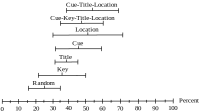
\includegraphics[width=.5\textwidth]{edmundson-score.pdf} % % %[width=140mm]
%% \caption{Mean co-selection scores of the features \citep{69-edmundson}.}
%% \label{fig:edmundson-score}
%%\end{center}
%%\end{figure}
%Most systems use different features combined together (linear combination, generally) to get a unique score. 
%The features weights can be fixed manually or using machine learning techniques described in a later section.
%%
%Also, other methods such as optimization can be used. 
%For instance, \citep{17-feigenblat-al} propose an unsupervised query-focused multi-document summarization method based on Cross-Entropy (CE) method \citep{04-rubinstein-kroese}. 
%It seeks to select a subset of sentences that maximizes a given quality target function using some statistical features.


\section{Graph-based approach}

%Introduce Graph-based approach
Inter-cohesion between text units (sentences) is an important property; A summary which contains linked units has the chance to be more pertinent to the input document's main topic.
Graph-based approach is based on transforming documents units (sentences, paragraphs, etc.) into a graph using a similarity measure, then this structure is used to calculate the importance of each unit. 
We divide graph-based works into two categories: those using graph properties such as the number of neighbors, and those iterating over the graph and changing nodes' scores till reaching a stable graph representation.

\subsection{Graph properties}

In \citep{97-salton-al}, document paragraphs are used to construct a graph of similarities, where each paragraph represents a node.
A paragraph is connected to another when their similarity is above a given threshold.
The authors define a feature called bushiness which is the number of a node's connections. 
The most scored paragraphs in term of bushiness are extracted to form a summary.

Node's bushiness can be used to score sentences alongside other statistical features \citep{09-abdelfattah-ren}.
In a graph of similarities between sentences, the importance of a sentence is the number of arcs connected to it.
Equation~\ref{eq:abdelfattah-arcs} represents the score based on number of arcs, where $ G =  \{S, A\} $ is the graph of similarities between the sentences, $ S $ is the set of sentences and $ A $ is the set of arcs.
\begin{equation}
	\label{eq:abdelfattah-arcs}
	Score_{\#arcs}(s_i) = |\{ s_j : a(s_i, s_j) \in A / s_j \in S, s_i \neq s_j \}|
\end{equation}

Beside bushy path of the node, \citet{14-ferreira-al} define another property called ``Aggregate Similarity". 
Instead of counting the number of arcs connected to a node, their weights are summed to represent this node's importance.
In their work, the authors investigate the fusion of multiple features, either graph-based or sentence features.

\subsection{Iterative graph}

LexRank \citep{04-erkan-radev} and TextRank \citep{04-mihalcea-tarau} are the most popular methods using graph-based summarization approach. 
The two methods use a modified version of PageRank \citep{98-brin-page} in order to score sentences. 
%
LexRank method \citep{04-erkan-radev} uses cosine similarity to construct a weighted graph where the nodes with a weight (similarity) less than a given threshold are omitted. 
Their method's continuous version follows almost the same equation as of TextRank, but it uses a \ac{tfidf} based cosine similarity instead.
%\begin{figure}[!ht]
%	\begin{center}
%		\includegraphics[width=.5\textwidth]{figures/approaches/graph.pdf} % % %[width=140mm]
%		\caption{An example of a graph representing similarities between sentences \citep{04-erkan-radev}.}
%		\label{fig:graph}
%	\end{center}
%\end{figure}
%
In TextRank, an undirected graph is constructed from the input text, where each sentence represents a node, and the arc between two nodes is weighted by their similarity. 
Equation \ref{eq:textrank} scores each sentence $ i $ based on its neighbors.
It is executed recursively till reaching convergence, where $ d $ is the damping factor (usually around $ 0.85 $).
\begin{equation}
	\label{eq:textrank}
	WS(V_i) = ( 1 - d) + d * \sum\limits_{V_j \in In(V_i)} \frac{w_{ji}}{\sum\limits_{V_k \in Out(V_j)} w_{jk}} WS(V_j)
\end{equation}
Where:
\begin{equation}
	\label{eq:textrank-sim}
	w_{ij} = \frac{|\{w_k \text{ / } w_k \in S_i \text{ and } w_k \in S_j\}|}{\log(|S_i|) + \log(|S_j|)}
\end{equation}

%Events
\citet{06-li-al} use PageRank to rank document events rather than sentences, then extract those sentences containing more important events.
They define an event as either a named entity (NE: Person, Organization, Location or Date), or an event term (ET: verb or action noun).
The relevance between two events is used to weight the arcs connecting them.
It is calculated as the number of associations in case of a pair of ET and NE.
In case of an ET pair, it is calculated as the number of NEs associated to both of them. 
Similarly, in case of an NE pair, it is the number of ET associated to both of them. 

%Temporal info
In case of multi-document summarization where there are some documents more recent than others, the temporal information matters. 
Recent documents contain novel information in an evolving topic.
Therefore, their sentences may be given more chance to be included into the summary. 
\citet{07-wan} proposes a method called TimedTextRank to incorporate this information into TextRank method.
The informativeness score ($ WS(V_j) $) is time-weighted, multiplying it by $ 0.5^{(y - t_j)/24} $ where $ y $ is the current time and $ t_j $ is publication time of the document containing a sentence $ j $.

%Sentence to document relationship
TextRank and LexRank exploit sentence-to-sentence relationships to score them, under the assumption that they are indistinguishable.
But in multi-document summarization, a document may be more important than others and therefore its sentences must be favored over others.
\citet{08-wan} proposes adding a sentence-to-document relationship into the graph-based ranking process. 
In addition to documents impact on sentences, the author argues that even sentences in the same document must not be treated uniformly.
The position of a sentence and its distance to the document's centroid are two factors to be included in sentence score.


%Other visions
Most graph-based summarization methods \citep{04-mihalcea-tarau,04-erkan-radev,06-li-al,08-wan} are based on ranking algorithms developed for web-pages analysis, such as PageRank \citep{98-brin-page} and HITS \citep{99-kleinberg}. 
In their method called iSpreadRank, \citet{08-yeh-al} exploit activation theory \citep{68-quillian} which explains the cognitive process of human comprehension.
The idea is to construct a graph of similarities between sentences, score each sentence using some features (centroid, position, and First-sentence overlap), then spread the scores to the neighbors iteratively until reaching equilibrium.

%2011-balinsky-al here

%Machine learning 
Some works try to introduce machine learning into graph-based ATS. 
In \citep{08-liu-al}, a prior probability is incorporated into PageRank algorithm to introduce query relevance into graph-based approach. 
The prior probability $ p(s/q) $ is estimated using Naive Bayes where the relevance of a sentence $ p(s) $ is estimated using four features (Paragraph Feature, Position in Paragraph Feature, Mood Type Feature, and Length Feature), and the relevance of query having some sentences $ p(q/s) $ is estimated using shared named entities between a query and the sentences in the training corpus.
Then, this probability is introduced into the past LexRank equation (see Equation \ref{eq:textrank}) as in Equation \ref{eq:pprsum}.

\begin{equation}
	\label{eq:pprsum}
	WS(V_i) = d * p(V_i/q) + (1-d) * \sum\limits_{V_j \in In(V_i)} \frac{w_{ji}}{\sum\limits_{V_k \in Out(V_j)} w_{jk}} WS(V_j)
\end{equation}
This model can select sentences with high relevance to the query without loosing the ability to select those with high information novelty. 


\section{Linguistic approach}

Statistical approach uses some primary \ac{nlp} techniques such as word segmentation, stop word elimination and stemming which are used by information retrieval systems. 
In the contrary, linguistic approach uses more profound \ac{nlp} techniques (part-of-speech, rhetoric relations, semantic, etc.) to generate summaries either by extraction or by abstraction. 

\subsection{Topic words}

The presence of some words such as ``significant", ``impossible", etc. can be a strong indicator of the relevance of a sentence to the main topic \citep{69-edmundson}.
A dictionary can be prepared from a corpus to save three types of cue words: \textit{Bonus words} which are positively relevant, \textit{Stigma words} which are negatively relevant and \textit{Null words} which are irrelevant.
The score of a sentence  $ s_i $ based on this feature is the sum of the weight of every word $ w $ according to the dictionary, as indicated in Equation \ref{eq:edmundson-cue}.
%\begin{equation}
%\label{eq:edmundson-cue}
%Score_{cue}(s_i) = \sum_{w \in s_i}{cue(w)}
%\end{equation}
%Where:
%\[ 
%cue(w) = \left\lbrace 
%\begin{array}{lll}
%b > 0 & if & (w \in Bonus) \\
%\delta < 0 & if & (w \in Stigma) \\
%0 & otherwise & 
%\end{array} 
%\right. 
%\]
\begin{equation}
	\label{eq:edmundson-cue}
	Score_{cue}(s_i) = \sum_{w \in s_i}{cue(w)}
	\text{ where }
	cue(w) = \left\lbrace 
	\begin{array}{ll}
		b > 0 & \text{if } (w \in Bonus) \\
		\delta < 0 & \text{if } (w \in Stigma) \\
		0 & otherwise 
	\end{array} 
	\right. 
\end{equation}

In \citep{09-abdelfattah-ren}, the cue words are divided into two groups: positive keywords and negative keywords.
Positive keywords are defined as ``the keywords frequently included in the summary". 
The score of a sentence $ s_i $ using positive keywords is given by Equation \ref{eq:abdelfattah-cue+}.
\begin{equation}
	\label{eq:abdelfattah-cue+}
	Score_{cue}(s_i) = \frac{1}{|s_i|} \sum_{w \in s_i}{tf(w) * P(s_i \in S | w)}
\end{equation}
Where: 
$ P(s_i \in S | w) $ is the probability that a sentence $ s_i $ belongs to a summary $ S $ given the occurrence of the word $ w $, which can be estimated using machine learning. 
Accordingly, negative keywords are the words unlikely to be in a summary, thus $ P(s_i \notin S | w) $.

\subsection{Indicators}

\citet{81-paice} defines them as ``\textit{commonly occurring structures which explicitly state that the sentences containing them have something important to say about the subject matter or the message of the document}";
For example, ``the principal aim of this paper is to investigate ...".
The identification of such indicators is not an easy task; in his work, the author followed these steps:
\begin{itemize}
	\item We cannot list all the indicators due to their variations.
	For example, these expressions have the same structure: ``This article is concerned with ...", ``Our paper deals with ...", ``The present report concerns ..." and ``The following discussion is about ...". 
	So, the solution is to use some templates.
	
	\item Using templates, some sequences of words which are not part of the indicators themselves may show up.
	The solution is to use skip limits between the paradigms of a given template.
	
	\item There exists optional words, but can add a weight when be used, such as the word ``here" in the expression ``The purpose \textbf{here} is to ...". 
	This can be addressed by defining multiple paths in the template.
	
	\item To handle the variations of words, their stems can be used in the templates instead.
	
\end{itemize}
Figure~\ref{fig:paice-template} represents a template, where the words or stems are paradigms.
The skip limits are shown thus: [3].
Weight increments are shown thus: +2.
A query (?) denotes an optional paradigm. 

\begin{figure}[!ht]
	\begin{center}
		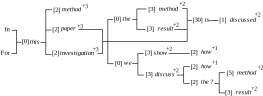
\includegraphics[width=.7\textwidth]{figures/approaches/paice-template.pdf} % % %[width=140mm]
		\caption{A slightly simplified template \citep{81-paice}.}
		\label{fig:paice-template}
	\end{center}
\end{figure}


\subsection{Co-reference information}

%Some works use statistical approach to calculate the score, but they use linguistic techniques for that, so we can consider them as linguistic ATS systems.
Some language-dependent properties such as part of speech, anaphora resolution, etc. can be used to enhance statistical approach. 
Although such works are using statistics to score a unit (sentence), we classify them as linguistic approach.
In the work of \citet{07-orasan-stafford}, the authors try to use anaphora resolution to improve the  informativeness of summaries.
Sentences, usually, contain pronouns rather than words which lead to incorrect score calculation. 
Anaphora resolution will increase the frequencies of words referred by these pronouns, and produces more accurate frequency counts.
The authors use a simple term frequency algorithm to score sentences, and six anaphora resolution methods.
The average informativeness was improved using anaphora resolution.

Semantic representations of terms are often used to generate summaries. 
Using ontologies and lexicons like Wordnet \citep{95-miller}, the semantic relationship between sentences' words can be exploited to enhance summary generation.
\citet{08-hennig-al} train an \ac{svm} classifier to identify salient sentences using ontology-based sentence features. 
This classifier is used to map the sentences to a taxonomy created by the authors, where each sentence is assigned a set of tags.
For each sentence, the tags are used to calculate the similarity with the document tags to determine how well a sentence represents the information content of its document in the ontology-space.
%- ENHANCE add a picture from 08-hennig-al

\subsection{Rhetorical structure}

The structure of discourse can be exploited through rhetorical relations between sentences to generate summaries. 
\citet{94-ono-al} use a penalty score defined over different rhetorical relations to exclude non-important sentences.
In \citep{98-marcu}, a discourse tree is built to reflect the rhetorical relations between the text's sentences as illustrated in Figure~\ref{fig:rhet-tree}, where the leafs are sentences.

\begin{figure}[!ht]
	\begin{center}
		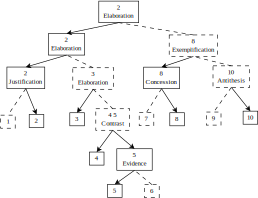
\includegraphics[width=.5\textwidth]{figures/approaches/rhet-tree.pdf} % % %[width=140mm]
		\caption{An example of a rhetorical tree \citep{98-marcu}.}
		\label{fig:rhet-tree}
	\end{center}
\end{figure}
The author uses seven metrics based on the rhetorical tree to find the best discourse interpretation similar to those of summaries: The clustering-based metric, the marker-based metric, the rhetorical-clustering-based metric, the shape-based metric, the title-based metric, the position-based metric and the connectedness-based metric.


\citet{14-kikuchi-al} propose a single document \ac{ats} based on nested tree structure. 
The authors exploit words dependency and rhetorical dependency  by constructing a nested tree composed of a document tree and a sentence tree. 
The document tree has sentences as nodes and head modifier relationships between sentences obtained by \ac{rst} as edges. 
The sentence tree has words as nodes connected by head modifier relationships between them obtained by the dependency parser.
The summarization is formulated as combinatorial optimization problem in order to trim the nested tree.

A more recent work using \ac{rst} is the work of \citet{16-goyal-eisenstein}, to fix the problems of local inference techniques which do not capture document-level structural regularities, and annotated training data.
So, the authors investigated the use SampleRank \citep{11-wick-al} structure learning algorithm as a potential solution to both problems.

\section{Machine learning (ML) approach}

Usually, machine learning approach is coupled with other approaches to improve and estimate their generation rules instead of fixing them manually.
It can solve the problem of combining features in statistical approach.
Many works have been conducted to generate summaries using machine learning, some focus on the choice of appropriate classification methods \citep{95-kupiec-al,02-osborne,05-yeh-al}, some try to solve the problems related to training phase, such as the absence of labeled corpora \citep{02-amini-gallinari}, others use heterogeneous features in their algorithms and try to combine them using machine learning \citep{08-wong-al,10-yatsko-al}. 

\subsection{As a tuning function}

\ac{ml} can be used with other approaches to tune certain parameters. 
It is mostly accompanied with statistical approach to solve the problem of estimating features weights, where these features scores are combined linearly into one score.
\citet{05-yeh-al} propose a method using genetic algorithm to estimate the features weights (sentence position, keywords, centroid and title similarity). 
Training a system on a corpus makes it dependent to the corpus's genre. 
A solution is to tune the features according to the input document's genre as suggested in \citep{10-yatsko-al}. 
45 features are used to train the system on three genres: scientific, newspaper, and artistic texts. 
The system can detect the genre of the input document and execute the adequate model of scoring. 

\subsection{As a decision function}

Given a corpus of documents with their extractive summaries, a machine learning algorithm can be used to decide if a unit (sentence mostly) belongs to the summary or not.
\citet{95-kupiec-al} propose an ATS system based on Bayes classification, in order to calculate the probability that a summary may contain a given sentence.
So, for each sentence $ s_i $, the probability that it belongs to a summary $ S $ using a features vector $ \overrightarrow{f} $ is given in Equation \ref{eq:bayes-kupiec}.
\begin{equation}
	\label{eq:bayes-kupiec}
	P(s_i \in S | \overrightarrow{f}) = %
	\frac{\prod\limits_{j = 1}^{|\overrightarrow{f}|} P(f_j | s_i \in S) * P(s_i \in S)}
	{\prod\limits_{j = 1}^{|\overrightarrow{f}|} P(f_j)}
\end{equation}
Where: 
$ P(s_i \in S) $ is a constant (so it can be emitted, since the probability is used for reordering), $ P(f_j | s_i \in S) $ and $ P(f_j) $ can be estimated from a corpus.
%
Choosing the right classification algorithm is another issue; for instance Bayes classification supposes features independence, which is not always the case.

From this point of view, \citet{02-osborne} uses a maximum entropy based classifier which, unfortunately, performs lower than Bayes' because it tends to reject a lot of sentences; but when he adds a prior probability, the method performs well and surpasses Bayes-based method.
His method, though, is not used to reorder sentences using the probability, but to classify them into two classes: summary sentences and other sentences.

\subsection{Bayesian topic models}

Topic models are based on identifying the main concepts from the input document(s) and find the relationship between them to construct a hierarchy. 
Words of each input document are assigned to a given number of topics, where a document is a mixture of different topics and each topic is a distribution of words. 
Bayesian topic models are quite sophisticated for multi-document summarization since they make difference between documents in contrast to most ATS methods which consider them as one giant document \citep{11-nenkova-mckeown}.
One of Bayesian topic models' advantages is their simplicity to incorporate different features, such as cue phrases used in \citep{08-eisenstein-barzilay} for unsupervised topic segmentation.


\citet{06-daumeiii-marcu} propose a query-driven muli-document summarization method using Bayesian topic models which is reported in \citep{11-nenkova-mckeown} as one of the first works in this direction.
In their method, the authors train their system to have three probability distributions: general English learning model ($ P^G $), background document language model ($ P^D $) for each one of the $ K $ available documents with $ S $ number of sentences and $ N $ number of words $ w $ in a sentence, and query language model ($ P^Q $) for each query $ q $ over a set of $ J $ queries.
Using this trained model, they estimate $ \pi $ using Expectation propagation \citep{01-minka}.
Figure~\ref{fig:btm-daumeiii} represents the graphical model of their method, where $ r $ is the relevance judgment,  $ z $ is the word-level indicator variables, $ \pi $ is the sentence level degrees, and $ \alpha $ is a Dirichlet distribution as prior over $ \pi $.
\begin{figure}[ht]
	\begin{center}
		\includegraphics{figures/approaches/btm-daumeiii.pdf} % % %[width=140mm]
		\caption{Bayesian Query-Focused Summarization Model proposed in \citep{06-daumeiii-marcu}.}
		\label{fig:btm-daumeiii}
	\end{center}
\end{figure}


\citet{11-celikyilmaz-hakkani} introduces \ac{ttm} which models topics as two levels: low-level topics which are distributions over words, and top-level topics which are correlations between these lower level topics given sentences.
One problem with \ac{ttm} is its incapability to differentiate general words from specific ones given a query. 
A Sentence containing general words, which are more frequent in document clusters, must have more chance to be included into the summary. 
The authors present an enriched \ac{ttm} (ETTM) generative process to sample words from high-level topics leading to three words distributions: low-level topics over corpus specific words, high-level topics over corpus general words, and background word distributions.

\citet{15-yang-al} argue that using expert summaries to indicate only two levels of topics limits the practical applications of \citet{11-celikyilmaz-hakkani}'s model, because we can draw many latent topics from multiple documents.
The availability of reference summaries and their quality as golden standards are two other challenges to this method. 
Furthermore, TTM does not take word dependency in consideration. 
To address these limits, they propose a new method called \ac{ctm} which is based on Bayesian topic model \ac{ttm}, hLDA model \citep{10-blei-al}, topical N-grams \citep{07-wang-al}, with some concepts of graph models. 

\subsection{Reinforcement learning (RL)}

%define reinforcement learning
Before presenting some \ac{ats} works based on \ac{rl}, lets first introduce \ac{rl} briefly. 
Given an agent in an environment, the former interacts with the latter via perception and action \citep{96-kaelbling-al}.
At each interaction, the agent perceives the current state $ s $ of its environment, among the set of possible states $ \mathcal{S} $.
Based on $ s $, the agent choose an action $ a $ from the set of actions it can perform on that state $ \mathcal{A}(s) $.
Of course, applying an action will change the environment's state to a new one $ s' $ resulting in a reward $ r $.
The agent's job is to learn an optimal policy $ \pi^* $, mapping states to actions $ p(a/s) $, that maximizes some long-run rewards.


\citet{12-ryang-abekawa} consider \ac{ats} extractive approach as a search problem. 
To our knowledge, They are the first to model the problem of constructing a summary as a \ac{rl} problem.
The state $ s = (S, A, f) $ is represented as a tuple of the current summary $ S $, a history of applied actions $ A $ and an indicator $ f \in \{0, 1 \} $ showing if it is terminal or not.
Thus, the initial state is represented as $ s_0 = (\emptyset,\emptyset, 0) $.
The authors define a function $ s: \phi(s) \in \mathbb{R}^d $ on the state, which is based only on the summary's feature $ \phi'(S) $ as given in Equation~\ref{eq:ryang-features}.
\begin{equation}
\label{eq:ryang-features}
\phi(s) = \left\lbrace 
\begin{array}{ll}
(\phi'(S), 0)^T & L(S) \le K \\
(0, 1)^T & otherwise \\
\end{array}
\right. 
\end{equation}
Where, $ K $ is the maximum size of a summary, $ L(S) $ is the current size of the summary and $ (0, 1)^T $ indicates that the summary violates the size constraint. 
In their experiments, the authors represent $ \phi'(S) $ as a vector of the following features: Coverage of important words, Coverage ratio, Redundancy ratio, Length ratio and Position. 
There are two types of actions: insert a unit (sentence) $ x_i $ referred to as $ insert_i $ and finish referred as $ finish $. 
%So, given an instant $ t $, the two types of transactions from a state $ s_t $ to another $ s_{t+1} $ using an action $ a_t $ are given in Equation~\ref{eq:ryang-actions}
%\begin{equation}
%\label{eq:ryang-actions}
%\begin{matrix}
%s_t & a_t  & s_{t+1} \\ 
%&\\
%
%\begin{pmatrix}
%S_t\\ 
%A_t\\ 
%0
%\end{pmatrix} & 
%\overset{insert_i}{\rightarrow} & 
%\begin{pmatrix}
%S_t \cup \{x_i\}\\ 
%A_t \cup \{ insert_i\}\\ 
%0
%\end{pmatrix} \\
%
%&\\
%
%\begin{pmatrix}
%S_t\\ 
%A_t\\ 
%0
%\end{pmatrix} & 
%\overset{finish}{\rightarrow} & 
%\begin{pmatrix}
%S_t \\ 
%A_t \cup \{ finish\}\\ 
%1
%\end{pmatrix} 
%\end{matrix}
%\end{equation}
The agent is rewarded only when it is in finish state; It is rewarded by the summary score $ score(S_t) $ if it does not violate the size limit, and it is penalized by a given value $ R_{penalty} $ otherwise.
The reward is represented in Equation~\ref{eq:ryang-reward}.
\begin{equation}
\label{eq:ryang-reward}
r_{t+1} = \left\lbrace 
\begin{array}{ll}
score(S_t) & a_t = finish \text{ and } L(S_t) \le K \\
- R_{penalty} & a_t = finish \text{ and } L(S_t) > K \\
0 & otherwise \\
\end{array}
\right. 
\end{equation}
The score of a summary $ S $ is a trade-off between its relevance $ Rel $ and redundancy $ Red $ as shown in Equation~\ref{eq:ryang-score}. 
\begin{equation}
\label{eq:ryang-score}
Score(S) = \sum\limits_{x_i \in S} \lambda_s Rel(x_i) - \sum\limits_{x_i, x_j \in S, i < j} (1 - \lambda_s) Red(x_i, x_j)
\end{equation}
Where $ Rel(x_i) $ is the cosine similarity between $ x_i $ and the document $ D $ plus a position-based score, $ Red(x_i, x_j) $ is the cosine similarity between these two units, and $ \lambda_s $ is a trad-off parameter set to $ 0.9 $. 
The policy is represented as a conditional distribution $ p(a|s;\theta,\tau) $ based on Boltzmann selection, which is parameterized by $ \theta $ and a temperature parameter $ \tau $.
The probability is calculated using $ r $ and $ \phi(s) $.
The authors use $ TD(\lambda) $ algorithm which is based on \ac{td} learning to estimate $ \theta $.


\citet{15-rioux-al} base their work on the method of \citet{12-ryang-abekawa}. 
They use an improved version of \ac{td} called \ac{sarsa} which, in addition to modeling state space, it models actions space too. 
Their reward function is immediate at every action to help the learner get immediate feedback.
It is similar to that of \citet{12-ryang-abekawa}, but the similarity function uses bi-grams instead of \ac{tfidf} and it incorporates ROUGE score.
%
Likewise, \citet{15-henss-al} follow the same method but with some changes. 
They use a different reward function based on reference summaries $ H_D $ and a set of features including ROUGE score during training.
Given a summary $ S_t $, the reward after performing and action leading to a summary $ S_{t+1} $ can be expressed as in Equation~\ref{eq:henss-reward}.
\begin{equation}
\label{eq:henss-reward}
r_{t} = Score(S_{t+1}; H_D) - Score(S_{t}; H_D)
\end{equation}
Where $ Score $ is a linear combination of the features scores.
Instead of using \ac{td} learning, the authors use Q-Learning to determine the value of the partial summary and the value of adding a new sentence to a summary state.
%Their method learns one global policy for a specific summarization task instead of one policy for each document cluster.

\ac{rl} can, also, be combined with deep learning to generate extractive summaries \citep{18-wu-hu}. 
The authors define a deep neural network model which takes as input the document $ d = (s_1, s_2, ..., s_n) $ composed on $ n $ sentences.
The model outputs a victor of binary decisions $ Y = (y_1, y_2, ..., y_n) $ indicating whether a sentence $ s_i $ belongs to the summary or not.
After training this model with supervised learning, it is trained again using \ac{rl} in order to incorporate coherence.


\subsection{Deep learning (DL)}

\ac{dl} has gained a lot of attention recently, even among \ac{ats} community.
It is based on large \ac{nn} which, eventually, needs a huge amount of data to be trained. 
It has been used for both extractive and abstractive \ac{ats}. 
We will start by presenting some extractive methods, then some abstractive ones.
%extractive

In \citep{12-liu-al,15-zhong-al}, the authors propose a query-oriented multi-document \ac{ats} method based on a \ac{dl} model.
The model contains three parts: concepts extraction, reconstruction validation and summary generation.
Concepts extraction is an encoder with 4 \ac{nn} layers which is fed with a vector of \ac{tf} representing a vocabulary with length $ V $ based on words appearing in the document topic set $ D $. 
Reconstruction validation is a decoder with 3 \ac{nn} layers which aims to reconstruct the input vectors. 
The last layer of Concepts extraction part is used with dynamic programming to seek most informative sentences. 

\citet{14-denil-al} use a hierarchical ConvNet architecture (CNN) divided into a sentence level and a document level.
The sentence level learns to represent sentences using their words and the document level learns to represent the input document using the first level. 
Then, these representations are used to score how pertinent a sentence can be towards the entire document.
Figure~\ref{fig:14-denil-al} represents the architecture used to infer document embedding from word embedding. 
First, word embeddings are concatenated into a sentence matrix which is transformed into a single vector using some operations. 
Then, the sentence embeddings are concatenated and transformed into a vector representing the document.
%
\begin{figure}[!ht]
	\begin{center}
		\includegraphics[width=.7\textwidth]{figures/approaches/14-denil-al.pdf} % % %[width=140mm]
		\caption{Inferring document embedding from word embedding in \citep{14-denil-al}.}
		\label{fig:14-denil-al}
	\end{center}
\end{figure}

In \citep{15-cao-al}, a \ac{r2n2} is used to rank sentences for multi-document summarization. 
The authors use two types of hand-crafted features as inputs: word features and sentence features. 
This enables the system to learn how to score sentences based on a hierarchical regression process which uses a parsing tree to score sentence constituents such as phrases. 

Like \citet{15-zhong-al}, \citet{17-yousefiAzar-hamey} propose an extractive query-oriented summarization method based on deep learning but for single-document \ac{ats}.
The main difference is the use of an unsupervised approach with deep \ac{ae} which was used in \citet{15-zhong-al} as a word filter rather than a sentence ranker. 
The AE, in this case, can learn different features rather than manually engineering them.
Furthermore, the authors investigate the effect of adding random noise to the local word representation vector on the summary.

In \citep{17-ren-al}, a neural network of two levels using contextual relations among sentences is proposed to improve sentence regression's performance. 
The first level captures sentence representations using a word-level attentive pooling convolutional neural network. 
Then, the second one constructs context representations using sentence-level attentive pooling recurrent neural network. 
These learning representations and the similarity of a sentence with its context are used to extract useful contextual features. 
The authors train the system to learn how to score a sentence to fit the ground truth of ROUGE-2.

%abstractive
To our knowledge, \citet{15-rush-al} are the first to successfully apply deep learning to abstractive \ac{ats}. 
Their system called NAMAS\footnote{NAMAS code: \url{https://github.com/facebookarchive/NAMAS} [October 03, 2017]} performs well on ``DUC-2004 shared task" corpus despite being tested using ROUGE metric which, mostly, encourages extractive summaries. 
The method uses a local attention-based model to generate each word of the summary $ y $ conditioned on the input sentence $ x $.
To do that, the model is trained to estimate a probability $ p(y_{i+1}|y_c, x; \theta) $ of generating a word $ y_{i+1} $ from a fixed vocabulary $ \mathcal{V} $ constructed from the input text. 
The probability is conditioned by the input sentence $ x $, a sequence of $ C $ words representing the last generated words, and parameters $ \theta $ representing word embedding matrix and weight matrices.
This method shows some limitations when it comes to input document and summary's size. 
It processes only documents with a size of about 500 words and produces a very short summary (about 75 characters). 

The previous work only generates summaries using input document's vocabulary without introducing out-of-vocabulary words.
To tackle this limitation, \citet{16-nallapati-al} also use an attention model in their encoder-decoder.
When they decode, they use only words that appear in the source document following a method called ``Large Vocabulary Trick" (LVT) \citep{15-jean-al}. 
Then, to introduce new words, they add a layer of ``word2vec nearest neighbor" in the input. 
The decision whether to use a word from the input or a new word based on the context is guaranteed by another layer they call ``Switching Generator/Pointer" layer \citep{15-luong-al,15-vinyals-al}.


\citet{17-ling-rush} try to fix the problem of speed when long source sequences (document summarization) are processed using sequence-to-sequence models with attention.
So, they use a two layer hierarchical attention; Where the first layer's function is to select one or more important chunks from the input document using hard attention, then feed it/them into the second layer using sequence-to-sequence model.
They use reinforcement learning to train the hard attention model.
The method shows promise to scale up existing methods into larger inputs, but fails to beat the standard sequence-to-sequence model. 



%\section{Sentence compression}
%
%
%The compression or reduction of sentences is the elimination of non informative parts, especially when the sentence is too long.
%\citet{99-jing-mckeown} confirm that the compression is often used by professional summarizers. 
%In fact, they found out that 78\% of summaries sentences are borrowed from the original document, and that half of them have been compressed.
%
%In \citep{02-knight-marcu}, two statistical compression methods are proposed: using the noisy channel model, and using decision trees.
%The first method supposes that the input sentence was short but has been bloated with additional words. 
%For a given long sentence, a syntactic tree is produced to which a quality score is attributed.
%It is calculated using \ac{pcfg} scores and the probabilities of next sentence calculated with bi-gram language model. 
%They measure the likelihood of transforming a wide tree to a reduced one using statistics gathered from a corpus of documents and their summaries.
%The second method is based on decision trees used to learn the different rules to reduce sentences.
%
%Likewise, in their statistical compression method, \citet{07-Zajic-al} consider a sentence to be a headline distorted by adding other words to it. 
%They use \ac{hmm} to represent the problem and finding the headline which maximizes the likelihood of this headline generating the sentence. 
%This likelihood is estimated using probabilities that a word is followed by another in a corpus of English headlines taken from TIPSTER corpus. 
%The authors propose another rule-based method where they use a parser to get the syntactic representation of the sentence, used to remove some components such as temporal expressions, modal verbs, complimentizer \textit{that}, etc.
%The compression is executed iteratively by removing one component at a time, outputting the compressed sentence into the extraction module.
%
%Other methods have been proposed to improve sentences compression using not only one sentence but using similar sentences.
%In \citep{08-cohn-lapata}, instead of shortening the sentence by removing words or components, the authors introduce additional steps as substitution, reordering, and insertion.
%In \citep{10-filippova}, a method is proposed to summarize a group of related sentences to a reduced one.
%In this method, the sentences are represented by one graph which is used to generate a reduced summary by following the shortest path.
%
%Deep learning has been applied in order to compress sentences. 
%\citet{15-filippova-al} use \ac{lstm} in order to perform a deletion-based sentence compression. 
%The method performs very well either in term of readability or informativeness even without affording syntactic information (PoS, NE tags and dependencies).
%%
%The same method is used in \citep{17-hasegawa-al} to compress Japanese sentences, but with some changes. 
%These modifications are based on three Japanese language characteristics: 
%\begin{itemize}
%	\item frequent verbs are nominalized and nouns are abbreviated;
%	\item a non verb can be a root node
%	\item easily estimated subjects and objects are omitted
%\end{itemize}


\section{Discussion}

We based our taxonomy on resources dependency: is a method based on some corpora? does it depend on some language toolkits? how much calculation power it needs?
Our intention is to classify \ac{ats} methods based on resource availability and the effort they take to be implemented. 
In this section, we will try to discuss the capacity of each approach to support multilingualism.

Statistical features based methods were the first introduced in ATS. 
Features like term frequency, position and length are language independent and are good indicators of sentence relevance. 
A statistical approach does not need much language dependent tools; just some basic \ac{nlp} tasks such as sentence segmentation, tokenizaion, stop word elimination, and stemming. 
Mostly, it is easy to be implemented and does not need a lot of processing power.
The statistical features are combined together in hope to better capture a sentence's relevance. 
This leads to a more complicated problem which is how to combine them, and how much amount of influence of each one. 
The problem can be solved by combining them linearly, and set their weights through experiments using a corpus or estimate them using machine learning.
Either way, we will have another problem which is language dependency. 

Graph-based approach seeks to exploit the shared information between sentences. 
It is a bottom-up method which discusses the similarity problem from the perspective of content structure \citep{15-yang-al}. 
It can be language-independent using just lexical similarities (mostly, cosine similarity) and statistical features. 
But, some room for improvement can be done by considering more language dependent similarities such as semantic similarity. 
Also, the model can be improved using machine learning, by introducing prior probabilities into the equation, as in \citep{08-liu-al}.
Processing a great amount of text using iterative graphs can consume more processing power; this should be investigated to better understand how far this approach can go.

Linguistic approach is more powerful than the statistic one in term of expressiveness, because it integrates richer features of the input text. 
Also, it can be used either for extractive or abstractive summarization.  
The problem with this approach is the lack of appropriate NLP tools for certain languages. 
It can be as simple as using sentence components (verbs, nouns, etc.) as statistical features, or as hard as using sentence structure and its relationships with others to generate a new text. 
Mostly, it is harder to be implemented and takes more time to generate a summary. 
\citet{11-nenkova-mckeown} suggests using linguistic methods as a post-processing task to improve linguistic quality of the generated summary rather than a processing one.
According to the authors, it is unclear how much this approach can improve content selection compared to the methods using no linguistic relations. 

All approaches discussed previously can be ameliorated using machine learning (ML).
On the other hand, they can loose multilingual property unless the system is trained on as many languages as possible. 
Still the problem of corpus domain; training your system on news articles does not mean it can handle fiction as good as it does with news.
Also, collecting labeled corpora for one language can be a very hard work, let alone many languages. 
Some works seek to use unlabeled data, and some propose auto-supervised methods such as \citep{02-amini-gallinari}.

%Sentence compression seeks to get rid of non informative parts allowing us to have shorter sentences. 
%It can be used as a post-processing task after generating a summary, which will eliminate more redundancy and allows more space for other sentences to be included. 
%It is a language dependent task which cannot be used alone to have a summary, but in conjunction of other approaches.

We tried to summarize all the above discussion in Table~\ref{tab:app-comp}.
The table shows some advantages and disadvantages of each approach, some encountered problems and their eventual fixes.
\begin{table}[ht]
	\caption{Comparison between different ATS approaches.\label{tab:app-comp}}
	\begin{tabular}{p{.12\textwidth}p{.25\textwidth}p{.25\textwidth}p{.25\textwidth}}
		\hline\hline\noalign{\smallskip}
		
		Approach & pros (+) \& cons (-) & problems & fixes \\
		\noalign{\smallskip}\hline\noalign{\smallskip}
		
		%==============STATISTICAL================
		Statistical 
		& 
		+ less resources \newline 
		+ simple \& fast \newline
		- readability
		& 
		* features combination \newline
		* relevancy \newline 
		* redundancy in sentences
		& 
		* machine learning \newline
		* linguistic features \newline 
		* compression
		\\
		
		\hline\noalign{\smallskip}
		
		%==============GRAPH================
		Graph 
		& 
		+ less resources \newline 
		+ simple \newline
		+ coherence \newline
		- processing power
		& 
		* sentences similarity \newline 
		* sentences \& documents properties
		& 
		* tf-idf, semantic \newline 
		* statistical \& linguistic features, sentence-document similarity, temporal property
		\\
		
		\hline\noalign{\smallskip}
		
		%==============LINGUISTIC================
		Linguistic 
		& 
		+ more accurate  \newline 
		+ abstractive ATS  \newline 
		- resources (toolkits) \newline 
		- complex \newline
		- processing power
		& 
		* generation rules
		&
		* machine learning 
		\\
		
		\hline\noalign{\smallskip}
		
		%==============MT================
		Machine learning 
		& 
		+ deducing rules automatically \newline
		- lack of corpora \newline
		& 
		* labeled corpora \newline
		* corpora insufficiency
		& 
		* reinforcement learning \newline
		* corpora creation
		\\
		
		\hline\noalign{\smallskip}
		
%		%==============Compression================
%		Compression 
%		& 
%		+ less redundancy \newline
%		- sentence level
%		& 
%		* sentence level
%		& 
%		* fuse with other approaches as a post-processing task
%		\\
%		
%		\noalign{\smallskip}\hline\hline
	\end{tabular} 
\end{table}

\begin{savequote}[75mm] 
	Good judgment comes from experience, and a lot of that comes from bad judgment.
	\qauthor{Will Rogers} 
\end{savequote}

\chapter{Summarization evaluation}
\label{chap:eval}


Evaluating summarization systems is one of the most difficult tasks. 
It is not clear which is the perfect summary, since humans produce different summaries and yet we can consider them all good. 
Also, the evaluation must be accurate, objective and fast. 
This led to the appearance of many evaluation methods which can be automatic, manual or semi-automatic. 
Many workshops have been organized to evaluate the performance of summarization methods, and test how effective evaluation methods are.

In this chapter we will present some evaluation methods, both intrinsic and extrinsic ones. 
The intrinsic ones seek to evaluate a system in of itself, while the extrinsic ones search to determine the effect of summarization on other tasks.
Then, we will enlist some famous evaluation workshops and campaigns in the context of \ac{ats}. 
Finally, we will discuss these evaluation methods focusing on their advantages and limits.

\section{Evaluation methods}

\ac{ats} evaluation methods can be considered as intrinsic or extrinsic \citep{01-mani}.
Intrinsic evaluation is meant to evaluate the system in of itself. 
It is based on two criteria: summary coherence and summary informativeness. %These criteria are explained later
In the other hand, extrinsic evaluation seeks to determine the effect of summarization on other tasks. 
Figure \ref{fig:eval-classif} represents the different categories of summarization evaluation, as described in \citep{01-mani}.
%
\begin{figure}[!ht]
	\begin{center}
		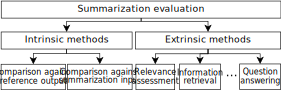
\includegraphics[width=.75\textwidth]{figures/evaluation/eval-classif.pdf} % % %[width=140mm]
		\caption{Classification of evaluation methods.}
		\label{fig:eval-classif}
	\end{center}
\end{figure}

\subsection{Intrinsic evaluation}

The evaluation can be done by comparing the generated summary to the original text or to a reference summary. 
When the system's summary is compared to the original text, actually, we look for the quantity of information recovered; more like information retrieval systems.
Comparing it to a reference summary will allow us to quantify how good the system can be against humans.
%two criteria of evaluation
Also, the intrinsic methods can be seen as: text quality evaluation methods or content evaluation methods \citep{12-steinberger-jezek}.
Text quality evaluation methods attempt to verify linguistic aspects of the generated summary such as grammaticality, reference clarity and coherence. 
The content evaluation methods can be divided into two sub-classes: co-selection methods which evaluate the system based on selecting the right sentences, and content based methods which go deeper by using smaller units such words and n-grams.

% .Recall, Precision, F-score
Given a summarizer which takes an input document $E$ and generates a summary $S$, and given a reference (model) summary $M$ which is some preselected sentences from $ E $; we can define the following relations: 
TP (true positive), TN (true negative), FP (false positive) and FN (false negative).
\begin{itemize}
	\item TP (true positive): the pertinent information captured by $M$ and $S$, so $M \cap S$.
	\item TN (true negative): the pertinent information not captured by $M$ and $S$, so $E - (M \cup S)$.
	\item FP (false positive): the pertinent information captured by $M$ and not captured by $S$, so $M - S$.
	\item FN (false negative): the pertinent information not captured by $M$ and captured by $S$, so $S - M$.
\end{itemize}
The recall is the quantity of right information recovered by a system comparing to what the it should recover (see Equation \ref{eq:recall}).
\begin{equation}
	\label{eq:recall}
	R = \frac {TP} {TP + FN} = \frac {M \cap S} {S}
\end{equation}
%
The precision is the quantity of right information recovered by a system comparing to what it has recovered (see Equation \ref{eq:precision}).
\begin{equation}
	\label{eq:precision}
	P = \frac {TP} {TP + FP} = \frac {M \cap S} {M}
\end{equation}
%
The F-Score is a mix between the recall and the precision using harmonic mean (see Equation \ref{eq:f-score}). 
If $ \beta $ is more than one (1), the recall is advantaged. 
If it is less than one, the precision is advantaged. 
The most used F-Score is F1-score which is a trade-off between recall and precision.
\begin{equation}
	\label{eq:f-score}
	F_{\beta} = \frac
	{(1+\beta^2) P \times R}
	{ \beta^2 P + R}
\end{equation}
We have to say, this type of evaluation does not give systems credit if they choose other sentences similar to the preselected ones. 
It may be useful to use when the summary must contain a precise information from the input text. 
But, in general, to evaluate a summarization system it must be avoided, especially for abstractive methods.

% .ROUGE
\acf{rouge}\footnote{ROUGE: \url{http://www.berouge.com/Pages/default.aspx} [November 23, 2016]}, proposed by \citet{03-Lin-hovy}, is a method inspired from another used for automatic translation evaluation called \ac{bleu} \citep{02-papineni-al}. 
The objective is to automatically measure the quality of the generated summary compared to a reference one.
The idea is to compute the number of units (N-grams) in both system's summary and reference one and calculate the recall.
Since a text can have many summaries, this method allows using many reference summaries.
Many variances of ROUGE have been proposed \citep{04-lin}: ROUGE-N, ROUGE-L, ROUGE-W, ROUGE-S, et ROUGE-SU. 
Equation \ref{eq:rouge-n} describes how ROUGE-N recall is calculated.
\begin{equation}
	\label{eq:rouge-n}
	ROUGE-(N) = \frac{\sum_{S \in Summ_{ref}}{\sum_{N-gram \in S}{Count_{match} (N-gram)}}}
	{\sum_{S \in Summ_{ref}}{\sum_{N-gram \in S}{Count (N-gram)}}}
\end{equation}
Where, \textit{N} is the size of the N-gramme, 
$count_{match}(N-gram)$ is the number of N-grammes found in both candidate and reference summaries. 
$Count (N-gram)$ is the number of N-grammes in the reference summary. 

% .Pyramids
Using similarity measure between automatic summary and human-made one can present some limitations \citep{07-nenkova-al}:
human variation, analyze granularity, semantic equivalence, semantic equivalence and the comparison between extractive and abstractive summaries.
\begin{itemize}
	\item Human variation: different people can select different sentences to incorporate into their summaries. 
	Even the same person can produce two different summaries for the same document.
	
	\item Analyze granularity: even if the system does not choose the same sentence as the model's, it can be pertinent to one sentence or plus in that model.
	
	\item Semantic equivalence: different sentences can express the same thing, even using different words.
	The annotators must choose one sentence out of equivalent sentences, and the system which choose two equivalent sentences must be penalized.
	
	\item Extractive or abstractive? Humans use abstractive summaries; A person use their own words to edit a summary.
	This is why the exact comparison between the reference's and the system's summaries is not possible.
	
\end{itemize}
Pyramid \citep{07-nenkova-al} comes to solve these limitations using a semi-automatic approach. 
Given a number of reference summaries, annotators are asked to define \acp{scu} where the weight of each \ac{scu} can be calculated as the number of relative reference summaries. 
The process of defining the \acp{scu} is not given, they can be as small as modifiers of a noun phrase or as large as a clause. 
The \acp{scu} are regrouped in a pyramid of $ n $ tiers, where $ n $ is the maximum weight of \acp{scu}. 
So an \acp{scu} which belongs to the tier $ T_i $ will have a score of $ i $, where $ |T_i| $ is the number of SCUs in this tier.
For a summary with $ X $ \acp{scu}, Equation \ref{eq:pyramid} shows the optimal content score, where \acp{scu} which do not belong to the pyramid will have a zero weight.
\begin{equation}
	\label{eq:pyramid}
	\max = \sum\limits_{i=j+1}^{n} i * |T_i| + j * (X - \sum\limits_{i=j+1}^{n} |T_i|),
	\text{ where } j = \max\limits_i (\sum\limits_{t = i}^{n} |T_t| \ge X)
\end{equation}

% .BE
\acp{be} are minimal semantic units which can be extracted from a sentence \citep{06-hovy-al}. 
Their goal is to automate summaries evaluation in contrast of Pyramids which needs human involvement. 
This later can introduce some problems such as human variability and evaluation expensiveness in time and cost.
To evaluate a summary, three different modules are proposed: \ac{be} breakers, \ac{be} matchers and \ac{be} scorers. 
The first one is used to break the text into \acp{be} which are defined by \citep{06-hovy-al} as:
``\textit{1- The head of a major syntactic constituent (noun, verb, adjective or adverbial phrases), expressed as a 	single item, or, 2- A relation between a head-BE and a single dependent, expressed as a triple (head | modifier | relation)}".
The matching of \acp{be} is either lexical, using lemmas, using synonyms from Wordnet \citep{95-miller}, using paraphrases or using semantic generalization.
Each BE gets a weight of 1 point for each related reference summary.

% .MeMoG and .AutoSummENG
\ac{autosummeng} \citep{06-giannakopoulos-al} attempts to be language neutral, fully automatic and context sensitive.
The method is based on n-grams, so to be language neutral no preprocessing must be done, this is why the n-grams are extracted over the characters.
Then, a graph is constructed where the n-grams represent its nodes and each arc connecting two n-grams is the number of times these n-grams are judged as neighbors given a distance window $ D_w $. 
Given two summaries $ S_i $ and $ S_j $ with a set of graphs $ \mathbb{G}_1 $ and $ \mathbb{G}_2 $ respectively, and given two graphs $ G^i \in \mathbb{G}_1 $ and $ G^j \in \mathbb{G}_2 $ with the same rank of n-grams, the value similarity is given in Equation~\ref{eq:val-sim}.
\begin{equation}
	\label{eq:val-sim}
	VS(G^i, G^j) = 
	\frac{\sum_{e \in G^i} \left(\mu(e, G^j) * \frac{min(w_e^i, w_e^j)}{min(w_e^i, w_e^j)}\right)}{max(|G^i|, |G^j|)}
\end{equation}
With $ \mu $ as the membership function, which returns 1 when $ e \in G^j $ and 0 otherwise.
$ w_e^i,\ w_e^j $ are the weights of the edges of the element $ e $ in the graphs $ G^i,\ G^j $ respectively.
The overall similarity of $ \mathbb{G}_1 $ and $ \mathbb{G}_2 $ is the weighted sum of the $ VS $ over all ranks (Equation \ref{eq:oval-sim}).
\begin{equation}
	\label{eq:oval-sim}
	VS^O(\mathbb{G}_1, \mathbb{G}_2) = 
	\frac{\sum_{r \in [L_{min}, L_{max}] } r * VS^r }{\sum_{r \in [L_{min}, L_{max}]} r}
\end{equation}
Where $ r $ is the rank of n-grams; 
$ L_{min},\ L_{max} $ are the minimum and the maximum rank of n-grams; 
$ VS^r $ is the value similarity using the graphs with n-gram of rank $ r $.
The grade of a summary is the average of all its similarities with the reference summaries. 
\ac{memog} is somehow a variant of \ac{autosummeng}, where all the graphs of reference summaries are merged into one graph \citep{10-giannakopoulos-karkaletsis}.

% .NPowER.
\ac{npower} \citep{13-giannakopoulos-karkaletsis} is a combination of many of the past metrics via optimization. 
The idea is to create a method which stands as an independent judge to combine the different metrics grades into a better estimate. 
Machine learning (linear regression) is used to estimate the final grade. 
Given a vector of features $ \overline{x} \in \overline{X}  $ (here, \ac{rouge}, \ac{be}, etc.) and a target numeric feature $ y \in \mathbb{R},\ y = f(\overline{x}) $, where $ f $ is an unknown function (human scores or Pyramid scores), the idea is to estimate a combination function $ \tilde{f} $ as shown in Equation \ref{eq:npower}.
\begin{equation}
	\label{eq:npower}
	\tilde{f}: \overline{X} \rightarrow \mathbb{R}: 
	\sum (\tilde{f}(\overline{x}) - f(\overline{x}))^2 \rightarrow 0,\ \forall \overline{x} \in \overline{X}
\end{equation}

Based on the expansiveness of summarization systems evaluated by these past metrics, we can say that these metrics are meant for background systems. 
But, how about update systems? In case we want to evaluate automatic summaries in term of new information which they contain.
Nouveau-ROUGE \citep{11-conroy-al} is a method based on \ac{rouge} metrics to evaluate update summaries. 
The idea is to calculate ROUGE score between an original summary and an update one, then a high \ac{rouge} score indicates high redundancy.
In TREC temporal summarization task \citep{13-aslam-al}, many metrics are proposed to address this issue. 
Given an event (Wikipedia event pages), gold standard updates called nuggets are extracted  and annotated to form a set of nuggets $ \mathcal{N} $ such as a nugget $ n \in \mathcal{N} $ has the properties: the time-stamp of revision history $ n.t $ and the importance provided by assessors (0: no importance to 3: high importance) $ n.i $. 
The evaluation metrics are designed to measure the degree to which a system can generate these nuggets in a timely manner.
Each system must generate a summary $ S $ containing some updates, where an update $ u $ is a sentence length text ($ u.string $) having a time-stamp $ u.t $.
The earliest update $ u $ that match a nugget $ n $ is defined as $ M(n, S) = \text{\textit{argmin}}_{u \in S: u \approx n} u.t $.
Then, the inverse function is defined as $ M^{-1}(u, S) = \{ n \in \mathcal{N}; M(n, S) = u \} $.
The first metric is \textit{Expected Gain metric} (EG) which is similar to traditional notions of precision in IR evaluation (see Equation \ref{eq:eg}). 
When using latency discount, the chosen latency step was $ \alpha = 3600 * 6$ (6 hours).
%
\begin{equation}
	\label{eq:eg}
	%.EG(S) = \frac{1}{|S|} \sum\limits_{\{n \in N: M(n,S) \ne 0 \}} g(M(n,S), n)
	EG(S) = \frac{1}{|S|} \sum\limits_{u \in S} G(u, S)
\end{equation}
Where, 
\[
%G(u, n) = \sum\limits_{n \in M^{-1} (u, \mathcal{S})} g(u, n)
G(u, n) = \sum\limits_{n \in M^{-1} (u, S)} R(n) * \text{\textit{discounting factor}}
\]
%\[
%g(u, n) = R(n) * \text{\textit{discounting factor}}
%\]
\[
R(n) = \left\lbrace\begin{tabular}{ll}
Graded:& $ \frac{e^{n.i}}{e^{\max_{n' \in \mathcal{N}} n'.i}} $ \\
Binary:& $ 1 $ if  ($ n.i > 0 $), $ 0 $ otherwise
\end{tabular}\right.
\]
\[
\textit{discounting factor} = \left\lbrace\begin{tabular}{l}
Discount-free gain: $ 1 $ \\
Latency-discounted gain: $ L(n.t, u.t) = 1 - \frac{2}{\pi} \arctan(\frac{u.t - n.t}{\alpha}) $ 
\end{tabular}\right. 
\]
%
Another metric is \textit{Comprehensiveness metric} C(S) which is similar to traditional notions of recall in IR evaluation (see Equation \ref{eq:cs}).
\begin{equation}
	\label{eq:cs}
	C(S) = \frac{1}{\sum_{n \in \mathcal{N}} R(n)} \sum\limits_{u \in S} G(u, S)
\end{equation}


\subsection{Extrinsic evaluation}

\ac{ats} is, often, used to complete other tasks like executing instructions, information retrieval, question answering, relevance assessment, etc. 
To evaluate how well a summarization system is doing leads to evaluate its effectiveness towards its related task. 
In the relevance assessment task, the assessors try to score how well a summary is related to a given subject.
Another example is reading comprehension task where a human judge is asked to answer some questions based on the original document, then on its summary.
The correct answers number is considered as the score of this summary.

%. SUMMAC extrinsic task
In TIPSTER SUMMAC evaluation \citep{99-mani-al}, two tasks are proposed to evaluate the impact of \ac{ats} on real world tasks: ad-hoc task and categorization task. 
In ad-hoc task, the purpose is to test the pertinence of indicative summaries towards a particular topic.
Given a document (summary or source text), a human subject is asked to determine its relevance to a given topic description, ignoring whether it was a full text or a summary.
The accuracy of the subjects is measured on how well they can indicate the relevance between the subjects and their relative full texts. 
Then the recall, precision and F1-score are calculated for the participants systems. 
In categorization task, the purpose is to determine if a generic summary contains enough information to allow an analyst categorizing a document as quickly and correctly as possible. 
The evaluation is proceeded as in ad-hoc task's.
But after reading the document, the human subject has to choose one category out of five or choose ``None of the above". 
Then the three measures: recall, precision and F1-score are calculated.
%Note: you can add the contengency tables

%. TODO DUC extrinsic task (dont't incorporate it)
%In DUC 2007 the pertinence to a topic was evaluated by giving scores by human evaluators

To assess the usefulness of a summary, according to \citet{05-dorr-al}, the decision made by a human judge (subject) based on the summary must be compared to its own decision made on the full-text rather than to a gold standard.
This is motivated by the fact that the users judgments based on the original texts are more reliable than basing on gold standard judgments.
Given a summary/document pair $ (s,\ d) $, the function $ j(s,\ d) $ equals to:
\begin{itemize}
	\item $ 1 $: if the subjects have the same judgment on both $ s $ and $ d $.
	\item $ 0 $: if the subjects change their judgment between $ s $ and $ d $.
\end{itemize}
Equation \ref{eq:rel-pred} calculates the Relevance-Prediction score for a set of summary/document pairs $ DS_i $ in association with an event $ i $.
\begin{equation}
	\label{eq:rel-pred}
	\text{\textit{Relevance-Prediction}} (i) = \frac{\sum_{(s, d) \in DS_i} j(s,\ d)}{|DS_i|}
\end{equation}

Another relevance prediction example is TREC Real-Time Summarization (RTS\footnote{RTS evaluation: \url{http://trecrts.github.io/TREC2016-RTS-guidelines.html} [December 20, 2016]}) track.
The purpose of summaries is to afford the users with tweets that are relevant to their profiles, and are novel.
Given a profile and a set of retrieved tweets, the gain $ G(t) $ of each tweet $ t $ is 0 if the tweet is not relevant, 0.5 if it is relevant or 1.0 if it is highly relevant.
This gain is attributed by some users having the target profile.
Based on this, three metrics are defined: Expected gain (EG), Normalized Cumulative Gain (nCG) and Gain Minus Pain (GMP) which are described in Equation \ref{eq:rts}.
%\begin{equation}
%	\label{eq:rts}
%	\begin{tabular}{lllll}
%		$ EG = \frac{1}{N} \sum G(t) $ &,&
%		$ nCG = \frac{1}{Z} \sum G(t) $ &,&
%		$ GMP = \alpha * nCG - (1- \alpha) * P$
%	\end{tabular}
%\end{equation}
\begin{equation}
	\label{eq:rts}
	\begin{tabular}{l}
		$ EG = \frac{1}{N} \sum G(t) $ \\
		$ nCG = \frac{1}{Z} \sum G(t) $ \\
		$ GMP = \alpha * nCG - (1- \alpha) * P$
	\end{tabular}
\end{equation}
Where $ Z $ is the maximum possible gain (given the ten tweet per day limit);
$ N $ is the number of tweets returned; 
$ P $ (pain) is the number of non-relevant tweets that are pushed, and $ \alpha $ controls the balance between the gain and the pain (0.33, 0.5, and 0.66 are used). 


\section{Workshops and evaluation campaigns}

Many summarization methods have been proposed since the 50's. 
To compare summarization systems, it is crucial to evaluate them in the same conditions. 
To do this, evaluation tasks have been proposed by some workshops and evaluation campaigns.
The main idea is to evaluate summarization systems using the same corpora and the same evaluation workflow. 

%+=========================================
\subsection{TIPSTER SUMMAC}

It was launched in may 1998 by the US government, in order to evaluate \ac{ats} systems in a large scale.
Three evaluation tasks were defined, two extrinsic (adhoc and categorization tasks) and one intrinsic (question-answering) \citep{99-mani-al}:
\begin{itemize}
	
	\item \textit{The ad-hoc task:} It is intended for indicative summaries based on a specific topic. 
	Given a document (the evaluator do not know if it is a summary or a full text) and a description of a topic, the evaluator is asked to determine if this document is pertinent to the topic. 
	
	\item \textit{The categorization task:} Its aim is to measure the effectiveness of a generic summary (ignoring the topic) to afford enough information allowing an analyst to categorize a document as quickly and correctly as possible. 
	Given a document (the evaluator do not know if it is a summary or a full text), the evaluator must choose from five categories the one which is pertinent to the document, otherwise he choose ``\textit{No category}".
	
	\item \textit{Question-Answering task:} This task seeks to evaluate the summaries in term of their informativeness. 
	This later is calculated using the number of correct answers which can be found in a summary for some questions generated from the source text.
	Each automatic summary is compared manually to some answer keys for each input document, to decide if the answer is correct, partially correct or incorrect. 
	ARS (\textit{Answer Recall Strict}) and ARL (\textit{Answer Recall Lenient}) metrics were defined to measure accuracy (see Equation \ref{eq:answer-recall}).
	\begin{equation}
		\label{eq:answer-recall}
		\begin{tabular}{l}
		$ ARS = \frac{n1}{n3} $ \\
		$ ARL = \frac{n1 + (.5 * n2)}{n3} $
		\end{tabular}
	\end{equation}
	Where $ n1 $ and $ n2 $ are the numbers of correct and partially correct answers in the summary, and $ n3 $ is the number of questions answered in the key. 
\end{itemize}

\subsection{DUC/TAC}
\label{sssec:eval-duc}

In 2001, \acf{duc}\footnote{DUC: \url{http://duc.nist.gov/} [November 23, 2016]} was launched as evaluation series in the area of text summarization. 
The aim of this workshop is to move forward the summarization research and enable researchers to test their methods in large-scale experiments. \ac{duc} 2004\footnote{DUC 2004 tasks: \url{http://duc.nist.gov/duc2004/tasks.html} [September 15, 2019]} knew 5 evaluation tasks using newswire/paper documents from the TDT and TREC collections:
\begin{itemize}
	\item \textit{Task 1 - Very short single-document summaries}: 
	For each English document out of 50, a very short summary must be generated ($ <= $ 75 Bytes).
	
	\item \textit{Task 2- Short multi-document summaries focused by TDT events}: 
	For each set of English documents out of 50 sets, a short summary must be generated ($ <= $ 665 Bytes).
	
	\item \textit{Task 3 - Very short cross-lingual single-document summaries}: 
	For each English translation (automatic and manual) of 25 Arabic documents, a very short summary must be generated ($ <= $ 75 Bytes).
	
	\item \textit{Task 4 - Short cross-lingual multi-document summaries focused by TDT events}: 
	For each English translation (automatic and manual) of 25 Arabic document sets, a short summary must be generated ($ <= $ 665 Bytes).
	
	\item \textit{Task 5 - Short summaries focused by questions}: 
	For each set out of 50 English documents sets, a short summary must be generated ($ <= $ 665 Bytes) to answer the question in form "\textit{Who is X?}", where X is a name of a person or a group of persons.
\end{itemize}
The summaries which exceed the limit size are truncated, and no bonus is attributed to the summaries shorter than this.
The evaluation of tasks 1 to 4 uses \ac{rouge} as a metric (ROUGE-1, ROUGE-2, ROUGE-3, ROUGE-4, and ROUGE-L).
In task 5, the summaries are evaluated in term of quality and coverage using \ac{see}\footnote{SEE: \url{http://www.isi.edu/licensed-sw/see/} [November 23, 2016]}.
As for the pertinence to the question ``\textit{Who is X?}", human evaluators have been used.

DUC 2007 used AQUAINT corpus, which contains news articles from \textit{Associated Press}, \textit{New York Times} (1998-2000) and \textit{Xinhua News Agency} (1996-2000).
There have been two tasks: principal task and update task.
%
\begin{itemize}
	\item \textit{Principal task:} For each topic of 25 documents, the contestants must generate a 200 words summary to answer one or more questions.
	
	\item \textit{Update task:} The goal is to produce a 100 words multi-document summary as update, supposing that the user has already read the previous articles.
	In this task, there are three clusters: cluster A with 10 documents for which the generated summary is not an update, cluster B with 8 documents for which the summaries must assume the user has already read those of cluster A, and cluster C with 7 documents which are more recent than those of cluster B.
	
\end{itemize}
The principal task is evaluated using many criteria:
\begin{itemize}
	\item Linguistic form of each summary is evaluated manually using some criteria: grammar, non redundancy, references clarity, focus, structure and coherence.
	For each criterion, the evaluator must give a score between 1 (not good) and 5 (very good).
	
	\item The pertinence to a given topic is evaluated manually; For each summary, the evaluator must give a score between 1 (not good) and 5 (very good).
	
	\item For automatic evaluation ROUGE-2, ROUGE-SU4 and BE are used.
\end{itemize}
As for update task, each summary is evaluated automatically using ROUGE-2, ROUGE-SU4, BE, and Pyramid.

Since year 2008, \ac{duc} has been included into the \ac{tac} as ``summarization" track.
The aim of this track is to develop \ac{ats} systems that afford short, coherent summaries of document.
This task is meant to promote a deep linguistic analysis for \ac{ats}.
It contains two tasks: the former DUC's ``update task" \citep{08-dang-owczarzak}, and a new one called ``opinion summarization task".
In the opinion summarization task, each system must generate well-organized, fluent summaries of opinions about specified targets, as found in a set of blog documents.
The questions are not simple, hence the answer can not be a named entity.
The evaluation is conducted manually using a nugget Pyramid created during the evaluation of submissions to the QA task.

In 2010 TAC's summarization track, a new task called "Guided summarization" replaced ``update summarization" one.
In this task, each system has to generate a 100 words summary from 10 news articles for each topic, where the topic belongs to a predefined category.
There are 5 categories: accidents and natural catastrophes, crises, health and safety, endangered resources, investigations and trials.
For a given topic, the contestants have to generate 2 summaries (for 2 sets: A and B):
\begin{itemize}
	\item One for the set A, which is guided by a request.
	\item The second (for set B) is the same as set A, but the summary must take in consideration that the user has already seen the documents of set A.
\end{itemize}
Each category has some aspects which have to be covered by the summary (for example, WHAT? WHY? WHEN? WHERE?).
To evaluate the content of summaries, Pyramid method is used. 
Readability and global sensibility are evaluated manually giving a score between 1 (not good) and 5 (very good).

\subsection{NTCIR}

The first \ac{ntcir}\footnote{NTCIR: \url{http://ntcir.nii.ac.jp} [November 23, 2016]} workshop was held in Tokyo, 1999. 
It was, originally, designed to enhance research in Japanese text retrieval. %, but other languages were introduced later
The second edition (2000-2001) had a ``Text summarization" task, which aims to collect data for text summarization and evaluate \ac{ats} systems.
The data was gathered from newspapers articles which were summarized by hand, to be used for research purposes. 
Two types of summaries were produced: extractive summaries (which are the important sentences in the text) and abstractive summaries.
Two tasks were proposed: intrinsic evaluation which contains two subtasks (extractive and abstractive) and extrinsic evaluation.
The process of each task is as follows \citep{01-fukusima-okumura}:
\begin{itemize}
	\item \textit{Task A-1}: The aim is to extract pertinent sentences, where the number of the extracted sentences is  10\%, 30\%, 50\% of the original texts.
	
	\item \textit{Task A-2}: The aim is to generate simple abstractive summaries.
	The generated summaries must have a number of characters of 20\% et 40\% comparing to the original text.
	
	\item \textit{Task B}: In this task, the summaries are produced based on some requests. 
	For each request, the system has to search for one relevant document and use it to produce a summary. 
	The length of the summary is not limited, but it has to be simple.
\end{itemize}
As to evaluate each task, the following metrics are used:
\begin{itemize}
	\item \textit{Task A-1}: For each summary, the correct sentences are selected. 
	Then, the metrics: recall, precision and F1 score are calculated using the number of sentences as a unit.
	The final score of each system is the average of all summaries scores. 
	
	\item \textit{Task A-2}: Two ways are used, an evaluation based on the content and a subjective evaluation.
	In the first one, the distance between the two terms frequencies vectors representing the system's summary and the human summary is considered as the score.
	In the second one, human evaluators are asked to evaluate the summaries based on two criteria: coverage and readability, and give a score of 1 (very good) to 4 (very bad).
	Each one of them is given 4 summaries: 2 human summaries, the system's summary and a summary produced using LEAD method.
	
	\item \textit{Task B}: In this task, human evaluators are given the requests and the generated summaries.
	For each summary, they have to judge if it is relevant or not to the request.
	Recall, precision and F1 score measures are calculated for each system based on the number of pertinent summaries.
	One other measure is the time taken for each system to complete this task.
\end{itemize}


\subsection{MultiLing}

The Multiling workshop began as a task of \ac{tac} in 2011, which aims to evaluate language-independent summarization systems on many languages \citep{11-giannakopoulos-al}.
In this task, at least two languages out of seven must be processed by participant systems: Arabic, Czech, English, French, Greek, Hebrew and Hindi.
For each, it has to generate a summary of 240 to 250 words.
To create the test corpus, 10 topics are selected where every topic contains 10 news articles from Wikinews.
Then, these articles were translated to the other languages sentence by sentence.
To evaluate the generated summaries, the two types of evaluation are used:
\begin{itemize}
	\item Automatic evaluation: it aims to calculate the performance of the systems using some model summaries created by fluent speakers of each language.
	Three methods are used: \ac{rouge} (ROUGE-1, ROUGE-2, ROUGE-SU4), \ac{memog} and \ac{autosummeng}.
	
	\item Manual evaluation: 
	Overall responsiveness of a text is used, where each summary was given a score of 1 to 5 based on the content and the quality of the language.
	When it covers all the important aspects of the original text and remain fluent, it will be attributed the score 5.
	If it is unreadable, nonsensical or containing just trivial information, it will be attributed the score 1.
\end{itemize}
%In this task, there were 8 participants: CIST, CLASSY, JRC, LIF, SIEL IIITH, TALN UPF, UBSummarizer and UoEssex, plus the baseline and the topline.
The topline system uses the model summaries (thus cheating) to select relevant sentences as summaries from original texts. 
The baseline system uses the centroid, extracted from a bag-of-words of same topic documents, to extract sentences using cosine similarity. 

In 2013, MultiLing went from a simple task of \ac{tac} to a workshop, which aims to test and promote multilingual summarization methods.
There were three tasks: \ac{mms} \citep{13-giannakopoulos},  \ac{mss} \citep{13-kubina-all} and ``Multilingual summary evaluation".
The 7 past languages used in \ac{mms} were used again along with three new languages: Chinese,  Romanian and Spanish.
The test corpus contains 10 topics for French, Chinese and Hindi, and 15 topics for the remaining languages. 
The evaluation methodology was the same as the 2011's, plus two automatic metrics: ROUGE-3 and \ac{npower}.
%In this task, there were 5 participants: Maryland, CIST, Lancaster, WBU and Shamoon.
%
The single document task introduces 40 languages, with a corpus of 30 documents for each language, created from wikipedia's featured articles.
%The size of the summaries can't be found!!!!
To evaluate the summaries, automatic methods are used: ROUGE-1, ROUGE-2 and \ac{memog}.
%In this task, there were four teams with six systems.


Multiling 2015 had two more tasks: \ac{cccs} and \ac{onforums}.
In \ac{cccs} task \citep{15-favre-al}, every system must generate abstractive summaries from call center conversations between a caller and an agent. 
The summaries must contain the caller's problem and the solution afforded by the agent. 
A corpus of French and Italian conversations was used, along with English translations of these two which makes them 3 languages. 
The two submitted systems had a hard time beating the three proposed baselines using ROUGE-2 as metric. 
%
\ac{onforums} task \citep{15-kabadjov-al} seeks to bring automatic summarization, argumentation mining and sentiment analysis all together. 
The data is a collection of English and Italian news articles along with the corresponding top 50 comments.  
Each system must generate some links between the article sentences and the comment sentences. 
Four research groups submitted their systems which have been evaluated using crowd-sourcing where a human judge scores linked sentences based on relation, agreement and sentiment between them.

\subsection{TREC}

\ac{trec}\footnote{TREC: \url{http://trec.nist.gov} [November 23, 2016]} is a metrics-based evaluation of TIPSTER Text program, which started in 1992. 
It is co-sponsored by the \ac{nist} and U.S. Department of Defense.
Its purpose is to provide the necessary infrastructure for large-scale evaluation, which can support research within the information retrieval community.

%http://www.trec-ts.org/downloads
``\textit{Temporal Summarization}" is a task of \ac{trec} which started in 2013 and took place over 3 years.
The goal of this track is to develop systems for efficiently monitoring the information associated with a news event such as protests, accidents or natural disasters over time. 
The track has the following four main aims \citep{13-aslam-al}:
\begin{itemize}
	\item Developing low latency algorithms to detect sub-events,
	\item Modeling information reliability with a dynamic corpus,
	\item Understanding and addressing the sensitivity of text summarization algorithms in an on-line, sequential setting, and
	\item Understanding and addressing the sensitivity of information extraction algorithms in dynamic settings.
\end{itemize}
The track includes two tasks:
\begin{itemize}
	\item \textit{Sequential Update Summarization}: A system should emit relevant and novel sentences to an
	event. 
	A simulator is given as arguments the system to be evaluated, a time-ordered corpus, an event keyword query, the event start time and its end time.
	For each document in the time-ordered corpus, the system may choose the sentences relevant to the keyword query and novel comparing to the earlier timestamps.
	
	\item \textit{Value Tracking}: A system should emit accurate attribute value estimates for an event. 
	A simulator is given as arguments the system to be evaluated, a time-ordered corpus, an event keyword query, the event start time, the event end time and the event attribute. 
	First, the system is initialized with the query and the attribute to generate an initial estimated value. 
	Then, with every document, which is in the time-line, the system generate a new value along with the supporting sentence's ID if there is a change.
	
\end{itemize}
To evaluate the tasks, some metrics have been proposed (for detailed description and formulas, see \citep{13-aslam-al}):
\begin{itemize}
	\item The novelty and the relevancy of the updated summary to the event topic.
	The metric used to measure this is called the (normalized) Expected Gain metric
	($nEG(S)$).
	\item The coverage of the essential information for the event by the summary. 
	The metric used to measure this is called Comprehensiveness metric ($ C(S) $).
	
	\item The degree to which the information contained within the updates is outdated.
	This is measured by the Expected Latency metric ($ E[Latency] $).
	
\end{itemize}

Since 2016, The temporal summarization track was merged with microblog track to form a new track called \ac{rts} track.
\ac{rts} track\footnote{RTS: \url{http://trecrts.github.io} [November 23, 2016]} is meant to explore novel and evolving information needed by users in streams of social media posts such as Twitter.
To achieve this goal, the track includes two scenarios:
\begin{itemize}
	\item \textit{Push notifications}: 
	In this scenario (Scenario A), the system must send relevant posts to the user's mobile phone as soon as they are identified. 
	These posts must be relevant to the user's interest, in time and novel.
	
	\item \textit{Email digest}:
	In this scenario (Scenario B), the system must identify a batch of 100 tweets according to a specific topic in a daily frequency.
	The summaries must be relevant to the user's interest and novel.
	The results are uploaded to \ac{nist} server after the end of the evaluation.
\end{itemize}
%
The evaluation takes 10 days, where all systems must listen to the Twitter sample stream using Twitter streaming API. 
A list of interest profiles will be provided to systems.
To evaluate the systems performances, two approaches are used: ``\textit{Live user-in-the-loop assessments} which is used only for the first scenario, and ``\textit{Post Hoc Batch Evaluations}" used for both scenarios.
\begin{itemize}
	\item \textit{Live user-in-the-loop assessments}: 
	Each system must push a notification to the \ac{trec} \ac{rts} evaluation broker as soon as it identifies relevant content to the users interest. 
	These notifications are immediately delivered to the mobile phones of a group of assessors who judge them using interleaved approach \citep{16-qian-al}.
	The assessor can judge the tweets in-time or later and send back the results to the evaluation broker using a mobile application.
	Each tweet is attributed a mention as relevant, relevant but redundant or irrelevant.
	
	\item \textit{Post Hoc Batch Evaluations}:
	A common pool is constructed based on the scenario's submissions where the depth of the pool is determined using the number of submissions and available resources.
	Tweets are assessed based on relevance: not relevant (get a gain of 0.0), relevant (get a gain of 0.5) or highly relevant (get a gain of 1.0).
	Then, relevant tweets are semantically clustered into groups with substantively similar information, the same as \ac{trec} 2015 Microblog evaluation.
	For the first scenario, EG-1, EG-0, nCG-1, nCG-0 and GMP scores are used, besides the latency which is the mean and the median difference between the time the tweet was pushed	and the first tweet in the semantic cluster to which the tweet belongs. 
	For the second scenario, nDCG@10-1 and nDCG@10-0 are used.
	
\end{itemize}

\section{Discussion}

In this chapter, we presented different summarization evaluation methods which can be intrinsic or extrinsic. 
Intrinsic evaluation is used to judge the performance of a certain method based on the quality of generated summaries.
Basically, the generated summary is compared to a reference one or to the original text in order to test informativeness (coverage and conciseness). 
The summary is also tested based on its readability; whether it contains some unresolved references and if it is coherent.
Extrinsic evaluation evaluates the quality of certain tasks such as information retrieval, reading comprehension and question answering.


In both cases, the evaluation can be manual, automatic or semi-automatic. 
% manual evaluation
In case of manual evaluation, a summary is evaluated by some assessors to judge its quality. 
This type of evaluation excels when it comes to judge if a summary is grammatically correct, if it is coherent, if it performs well for a task, etc.
The dark side of manual evaluation is subjectivity; sometimes the evaluator's experience and point of views can affect their judgment. 
The quality of a good summary can vary from person to another.
Hopefully, there is a solution for this: a summary can be evaluated by many assessors, then the inter-rater agreement between them can be calculated (for example: Kappa coefficient) to verify how well they agree on the score.
Even so, the evaluation can take a long period of time, and the cost of hiring experts to evaluate the summaries can be high. 

% automatic evaluation
On the other hand, automatic evaluation can afford quick results with less or no cost at all. 
In general, it performs well when the evaluation concerns informativeness (coverage and conciseness). 
Many reference summaries of the same document are used in the evaluation since there exists not only one answer but many.
Unfortunately, automatic evaluation methods based on terms or n-grams, such as \ac{rouge}, tend to favor extractive summaries over abstractive ones.
When it comes to readability, automatic evaluation cannot stand a chance against manual one.
Readability, here, refers to references clarity, coherence and grammaticality and not the ease with which a reader can understand a well written text. 
The latter can be measured using automatic metrics such as Flesch–Kincaid readability tests \citep{75-kincaid-al} and SMOG \citep{69-laughlin-harry}.
% semi-automatic
Semi-automatic evaluation tries to take advantage of the two previous approaches' benefits. 
The idea is to automatically evaluate summaries when it is possible and delegate to humans the tasks they can do better.  
But, lets not forget that doing this can draw the two approaches' problems as well.


Mostly, summaries are used to enhance other tasks such as information retrieval or to help users pick the right document. 
A system's designer will focus on summaries' informativeness much more than their readability. 
In this case, automatic evaluation is more suitable since a summarization method can be evaluated quickly with low costs.
Probably, this is why it is the most used approach in workshops and evaluation campaigns. 
In the context of multilingual summarization, most automatic evaluation methods such as \ac{rouge} can be applied immediately to other languages without any change.
On the other hand, manual evaluation of a multilingual summarization method can be costly in term of time and money. 
For each language a system can handle, we must find an expert which must evaluate all the summaries generated from our test corpus. 





\begin{savequote}[75mm] 
The journey of a thousand miles begins with one step.
\qauthor{Lao Tzu} 
\end{savequote}

\chapter{Topic clustering and classification (TCC) for multilingual ATS}
\label{chap:tcc}


Clustering has been used for summarization in many systems, either using documents as units, sentences or words. 
The resulted clusters are used to extract the summary.
Some systems use just the biggest cluster to score sentences and get the top ones such as `UoEssex" system \citep{11-elhaj-al} which is justified by the assumption that a single cluster will give a coherent summary. 
Others take a representative sentence from each cluster, in order to cover all topics. 
While there are systems which score sentences according to all clusters.
%scoring
These three methods represent how each sentence is selected to be in the summary based on its cluster(s). 
But to score these sentences, we can divide the scoring methods into two groups: rule based and data driven. 
The former one rely on hand written rules to score sentences. % such as in ``CIST" and ``UoEssex" systems.
%``CIST" \citep{11-liu-al,13-li-al} uses \ac{hlda} model to cluster sentences into sub-topics.
%Then, the sentences of the largest sub-topic are scored using \ac{hlda} model combined with some traditional features. 
%Likewise, ``UoEssex" \citep{11-elhaj-al} uses K-Means to cluster similar sentences.
%Sentences of biggest cluster are scored using their cosine similarities to the cluster's centroid. 
On the other hand, data driven methods use machine learning to infer scoring or decision models. 
%For instance, ``CLASSY" system \citep{11-conroy-al} uses na\"ive Bayes to estimate the log-likelihood that a term may be included in the summary.

%Problems facing multilingual summarization
One of multilingual summarization's problem is the lack of resources such as labeled corpus used for training.
Machine learning algorithms were used either to select the sentences that should be in the summary, or to estimate the features' weights. 
Both cases need a training corpus given the language and the domain we want to adapt our summarizer to. 
To design a language-neutral summarization system, either we adapt our system to input languages (Partly language-neutral), or we design a system that can process any language (Fully language-neutral). 

In this chapter, we will present our method based on clustering and machine learning to score sentences in a multilingual fashion which is called \acf{tcc} \citep{13-aries-al,15-aries-al}. 
It will be used as a baseline in our other methods. 
%
In this method, we use a simple fuzzy clustering algorithm.
We assume that a sentence can express many topics, and therefore it can belong to many clusters.
Also, we believe that a summary must take in consideration other topics than the main one (the biggest cluster).
To score sentences, we use a scoring function based on Na\"ive Bayes classification. 
It uses the clusters for training rather than a corpus, in order to avoid the problem of language dependency.
Figure \ref{fig:gnrl-arch} represents the general architecture of AllSummarize\ac{tcc} method.

\begin{figure*}
	\begin{center}
		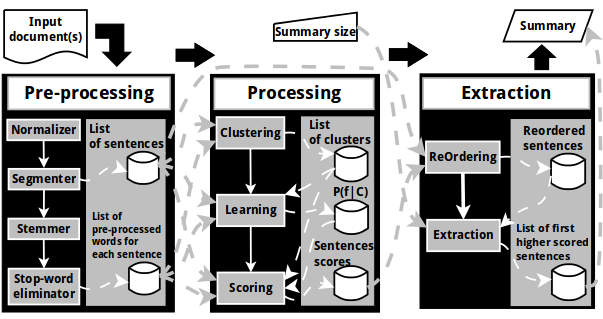
\includegraphics[width=\textwidth]{figures/tcc/gnrl-arch.pdf}
	\end{center}
	\caption{\label{fig:gnrl-arch} General architecture of AllSummarizer (TCC method).}
\end{figure*}


\section{Preprocessing}

This is the language-dependent part, which can be found in many information retrieval (IR) works. 
It is needed by the method but does not affect the fact that the method is language independent. 
Also, these tools are not difficult to be found for most languages since they are simple compared to other natural language processing tasks.
In our system, we are interested in these preprocessing tasks: Normalization, Segmentation, Stemming and Stop words removal.
%\begin{itemize}
%	\item Normalization	
%	\item Segmentation
%	\item Stemming
%	\item Stop words removal
%\end{itemize}


% Normalization
Normalization is the process of transforming a text into a canonical form. 
It is used to get one form especially for as acronyms, Abbreviations, dates and numbers. 
For instance, in a text, the author can write the number 4 as ``four" in some parts and as ``4" in others. 
In case of HTML text, tags has to be deleted before processing the text; otherwise, they will affect the task in question. 
Also, it can be used to delete special characters such  are diacritics (Tashkiil) in case of Arabic and  Persian. 
In our case, we use this task just for Arabic and Persian, since the diacritics create many variations of the same word. 
For instance, the word ``\textarab[voc]{عَمِلَ} \textit{/‘amila/ ([He] worked)}" and ``\textarab[voc]{عَمَلٌ} \textit{/‘amalun/ (work)}" can be treated as the same while processing.

% sentence segmentation
Text segmentation task is composed of two sub-tasks: sentence segmentation and words tokenization.
First of all, we must split the input text into several sentences mostly using punctuation. 
Detecting sentence boundaries using the period mark can fail when it meets some abbreviations such as: ``Dr.", ``Mr.", ``Ms.", ``PhD.", etc. 
Also, there exists some languages such as Thai which does not have a delimiter for sentences.
% words tokenization 
After segmenting each sentence apart, we must recover the list of words using a task called ``words tokenization".
Splitting a text into words is not as simple as using the blank (white space) as a separator. 
Languages such as Japanese and Chinese does not use blank character to separate the different words of a sentence. 
For instance, the Japanese sentence ``私の名前はカリムです。 \textit{/watashi no namae wa karimu desu./ (My name is Karim.)}" does not have any marks to distinguishing different words.

% stemming
Due to variations resulted from inflection or derivation of words, we end up with many variations of the same word. 
For instance, the word ``inspire" can have many derivations: ``inspirer", ``inspiration", etc. and conjugation forms: ``inspired", ``inspires".
The solution is to use stemming which aims to remove prefixes, suffixes and infixes in order to help associating variants of the same term with a common root form.

% stop words removal
Some words are better not to be included into the scoring process.
Among these words, we can mention: pronouns, prepositions, etc. which are independent from the subject of the text.
It is too easy to find a list of these words on the web for a given language.


% used tool
In our work, we use an open source tool (LangPi\footnote{LangPi: \url{https://github.com/kariminf/langpi}}) which we designed to afford these tasks for 40 languages.
Table \ref{tab:preprocess} shows each language and the tools used for each preprocessing task.
For more information about LangPi, check Appendix A.
%
\begin{table}[!ht]
	\centering
	\caption{Tools used to preprocess each language in LangPi}
	\readtable{tcc/preprocess.tex}
	\label{tab:preprocess}
\end{table}


\section{Topics clustering}

Each text contains many topics, where a topic is a set of sentences having some sort of relationship between each other.
In our case, this relationship is the cosine similarity between each two sentences. 
Which means, the sentences that have many common terms are considered as having the same topic. 
Given two sentences $ X $ and $ Y $, the cosine similarity between them is expressed by Equation \ref{eq:cosine}.

\begin{equation}
\label{eq:cosine}
cos(X,Y) = \frac {\sum_i {x_i.y_i} }
{\sqrt{\sum_i(x_i)^2} . \sqrt{\sum_i(y_i)^2}}
\end{equation}
Where $ x_i $ ($ y_i $) denotes frequencies of each term in the sentence $ X $ ($ Y $).
$x_i.y_i$ represents the multiplication of shared terms frequencies between X and Y.


To generate topics, we use a simple algorithm (see Algorithm  \ref{algo:cluster}) which is based on cosine similarity and a clustering threshold $ th $ to clustering $ n $ sentences.
The sentences having a similarity greater than $ th $ are regrouped into the same cluster. 
A sentence can belong to many clusters at once, this is motivated by the fact that a sentence can discuss many topics.

\begin{algorithm}[!ht]
	\readalgo{tcc/cluster.tex} 
	\caption{Clustering method used in AllSumarizer TCC}
	\label{algo:cluster}
\end{algorithm}



\section{TCC scoring function}

A summary is a short text that is supposed to represent most information in the source text, and cover most of its topics.
Therefore, we assume that a sentence can be in the summary when it is most probable to represent all topics (clusters)  using a set of features.
Assuming clusters independence, the probability of a sentence $ s_i $ representing all topics $ c_j \in C $ based on some features $ f_k \in F $ is given in Equation~\ref{eq:tcc-prob}. 
\begin{equation}
\label{eq:tcc-prob}
P(s_i \in \bigcap_{j} c_j | F) = 
\prod_{j} P(s_i \in C_j | F)
\end{equation}

If we assume features independence, using Bayes' theorem $ P(s_i \in C_j | F) $ can be calculated as indicated in Equation~\ref{eq:tcc-bayes}. 
Since the denominator (the evidence) does not depend on either clusters or features, it is effectively constant.
The evidence can be dropped from the equation since this probability is going to be used to reorder sentences.
\begin{equation}
\label{eq:tcc-bayes}
P(s_i \in C_j | F) = 
\frac{P(s_i \in C_j) . P(F | s_i \in C_j) }{P(F)} 
\propto 
P(s_i \in C_j) . P(F | s_i \in C_j)
\end{equation}

Combining this equation with Equation~\ref{eq:tcc-prob}, the probability $ P(s_i \in \bigcap_{j} C_j | F) $ can be represented as in Equation~\ref{eq:tcc-final-prob}.
Since we are multiplying all the priors ($P(s_i \in C_j)$), it can be deleted because the result will be constant.
On the other hand, Naive Bayes assumes features independence of each other.
\begin{equation}
\label{eq:tcc-final-prob}
P(s_i \in \bigcap_{j} C_j | F) \propto 
\prod_{j} \prod_{k} P(f_k | s_i \in C_j)
\end{equation}

To simplify combining various sentence features, especially those of term frequency, we propose to use a score rather than a probability.
Also, since the classification task used here is nothing but a scoring tool (which we use just to score the sentence in each cluster), using scores has the same purpose as using a probability.
So, the score of a sentence $ s_i $ is the product over classes and features of its score in a specific class and feature (see Equation. \ref{eq:globalscore}).
%
\begin{equation}
\label{eq:globalscore}
Score(s_i , \bigcap_{j} c_j , F) =  %\propto 
\prod_{j} \prod_{k} Score(s_i , c_j , f_k )
\end{equation}

The score of a sentence $ s_i $ in a specific cluster $ c_j $ and feature $ f_k $ is the sum of probability of the feature's observations when $ s_i \in c_j $ (see Equation. \ref{eq:score}).
We add one to the sum, to avoid multiplying by a features' score of zero.
%
\begin{equation}
\label{eq:score}
Score(s_i , c_j , f_k ) = 1 + \sum_{\phi \in s_i} {P(f_k=\phi | s_i \in c_j)}
\end{equation}
%
Where $ \phi $ is an observation of the feature $ f_k $ in the sentence $ s_i $.
For example, assuming the feature $ f_{k1} $ is term frequency, and we have a sentence: ``\textit{I am studying at home.}".
The sentence after preprocessing would be: $ s_i $ = \{``\textit{studi}"(stem of ``study"), ``\textit{home}"\}.
So, $ \phi $ may be ``\textit{studi}" or ``\textit{home}", or any other term.
If we take another feature $ f_{k2} $ which is sentence position, the observation $ \phi $ may take 1st, 2nd, 3rd, etc. as values.


\section{Training and statistical features}

We use 5 statistical features to score the sentences: unigram term frequency (TFU), bigram term frequency (TFB), sentence position (Pos) and sentence length (Rleng, PLeng).
We treat this features as categorical even if they are numerical. 
Thus, we will consider each 
For example, if we have a text written just with three characters: a, b and c, and the feature is the characters of the text, then we will have three categories.
Each category has a probability to occur in a cluster, which is the number of its appearance in this cluster divided by all cluster's terms, as shown in Equation \ref{eq:likelihood}. 
%
\begin{equation}
\label{eq:likelihood}
P_{f}(f = \phi | c_j) = \frac {|\{ \phi \in c_j \}|}{\sum_{c_l \in C}{| \{ \phi' \in c_l \} |}}
\end{equation}
Where $ f $ is a given feature.
$ \phi $ and $ \phi' $ are observations (categories) of the feature $ f $ .
$ C $ is the set of clusters.


\subsection{Term frequency}

This feature is used to calculate a sentence's pertinence based on its terms. 
We use two types of term frequency: Unigrams (TFU) and Bigrams (TFB). 
Unigrams (TFU) consider each term as a category.
While Bigrams (TFB) considers each pair of consecutive terms as a category.


\subsection{Sentence position}

We want to use sentence positions in the original texts as a feature. 
The position feature used by \citet{02-osborne} divides the sentences into three sets: the ones in the 8 first paragraphs, those in last 3 paragraphs and the others in between. 
Following the assumption that the first sentences and last ones are more important than the others. 

Three categories of sentence positions seem very small to express the diversity between the clusters.
Instead of just three categories, we divide the position space into 10 categories. 
So, if we have 20 sentences, we will have 2 sentences per category.
If we have 10 sentences, in single document each cluster will contain at most one occurrence of a given category.
But, in multi-document a cluster can contain sentences of the same position (in their original documents).


\subsection{Sentence length}

One other feature applied in our system is the sentence length (number of words), which is used originally to penalize the short sentences. 
Following a sentence's length, we can put it in one of three categories: sentences with length less than 6 words, those with length more than 20 words, and those with length in between \citep{02-osborne}.

Like sentence position, three categories is a small number. 
Therefore, we used each length as a category.
Suppose we have 4 sentences which the lengths are: 5, 6, 5 and 7, then we will have 3 categories of lengths: 5, 6 and 7.

In our work, we use two types of sentence length:
\begin{itemize}
	\item Real length (RLeng): which is the length of the sentence without removing stop-words.
	\item Pre-processed length (PLeng): which is the length of the sentence after pre-processing.
\end{itemize}


\section{Summary extraction}

To extract sentences, we reorder them using their scores in decreasing order.
Then, we extract the first non similar sentences until we get the wanted size (see Algorithm \ref{algo:extract}).
The next sentence to be added is compared to the last one accepted to the summary in order to decrease similarity between summary's sentences.
The logic behind this method is to select the most relevant sentences with less redundancy.

\begin{algorithm}[!ht]
	\readalgo{tcc/extract.tex}
	\caption{Extraction method using sentences similarities and their scores}
	\label{algo:extract}
\end{algorithm}


\section{Experiments}

These experiments have been held upon our participation in MultiLing'15 workshop \citep{15-aries-al}. 
We participated in all proposed languages, either in single document or multi-document tasks.
First, the participants have been provided by some training corpora to train their systems. 
In our case, we used the two training corpora to select the best parameters to maximizing ROUGE-1 score of our system's summaries. 
After that, the participants have been provided by some test corpora which contains just the original text (without the golden summary). 
They have to generate summaries using their systems and send them to the organizing members in order to evaluate them.

The systems should be able to exceed a simple baseline system which takes the first sentences as a summary. 
Since there is a baseline which specifies a lower score a system can have, there has to be a higher score an automatic summarizer cannot exceed. 
The oracle summary was generated by selecting sentences from the original text that covers the words in the summary using a minimal number of sentences until reaching summary's size. 

Contrary to our system, there are some which participated to a subset of the proposed languages. 
To compare our system against them, we followed these steps (for every evaluation metric): 
\begin{itemize}
	\item For each system, calculate the average scores of all used languages.
	\item For our system, calculate the average scores of used languages by others. 
	For example, BGU-SCE-M team uses Arabic, English and Hebrew; 
	We calculate the average of scores of these languages for this system and ours.
	\item Then, we calculate the relative improvement using the averages $ \frac{our system - other system}{other system} $.
\end{itemize}



\subsection{MultiLing 2015 corpora}

In our experiments we use MultiLing 2015 Multi-lingual Single-document Summarization (MSS) corpus which is designed for multilingual summarization. 
The corpus contains two parts: training data which is used to train the system, and testing data which is used to test the system's performance on unseen data.
For every part (training and testing) and for each language of 38 ones, 30 documents extracted from Wikipedia featured articles are afforded.
Featured articles are selected based on accuracy, neutrality, completeness, and style; which makes them a good source for this task.
For each summary which is UTF-8 encoded, a manual summary and its number of characters are afforded. 
The size of an automatically generated summary in term of characters must not exceed that number.
Table~\ref{tab:multiling15mss} represents some statistics on MultiLing 2015 Multi-lingual Single-document Summarization (MSS) corpora.

\begin{table*}[!ht]
	\centering
	\caption{MultiLing 2015 Multi-lingual Single-document Summarization (MSS) corpora statistics.}
	\readtable{tcc/multiling15mss.tex}
	\label{tab:multiling15mss}
\end{table*}

Also, we use MultiLing 2015 Multi-lingual Multi-document Summarization (MMS) corpus. 
It contains texts of ten different languages: Arabic, Chinese, Czech, English, French, Greek, Hebrew,
Hindi, Romanian and Spanish.
It is based on WikiNews English news articles which were translated into the other languages.
The corpus comprises 15 topics in which there are 10 documents. 
Three randomly chosen topics are reserved for the training phase, while the rest are leaved for the test.
Table~\ref{tab:multiling15mms} affords some statistics on MultiLing 2015 Multi-lingual Multi-document Summarization (MMS) corpora.

\begin{table*}[!ht]
	\centering
	\caption{MultiLing 2015 Multi-lingual Multi-document Summarization (MMS) corpora statistics.}
	\readtable{tcc/multiling15mms.tex}
	\label{tab:multiling15mms}
\end{table*}


\subsection{Summarization parameters}

In this section, we describe how the summarization parameters have been chosen.
The first parameter is the clustering threshold, which will lead to few huge clusters if it is small, and inversely.
The clustering threshold is used with sentences' similarities to decide if two sentences are similar or not.
Our idea is to use statistic measures over those similarities to estimate the clustering threshold.
Eight measures have been used: The median, The mean, The mode (lower and higher), $ sDn = \frac{\sum |s|}{|D| * n}$, $ Dsn = \frac{|D|}{n * \sum |s|}$ and $ Ds = \frac{|D|}{\sum |s|}$ .
%\begin{itemize}
%	\item The median
%	\item The mean
%	\item The mode which can be divided to two: lower mode and higher mode, since we can have many modes.
%	\item The variance
%	\item $ sDn = \frac{\sum |s|}{|D| * n}$ 
%	\item $ Dsn = \frac{|D|}{n * \sum |s|}$ 
%	\item $ Ds = \frac{|D|}{\sum |s|}$ 
%\end{itemize}
Where, $|s|$ is the number of different terms in a sentence $s$. 
$|D|$ is the number of different terms in the document $D$.
$n$ is the number of sentences in this document.
%
The second parameter is the features' set, which is the combination of at least one of the five features. 
We want to know which features are useful and which are not for a given language.

To fix the problem of the clustering threshold and the set of features, we used the training sets provided by the workshop organizers.
For each document (or topic in multi-document), we generated summaries using the 8 measures of $ th $, and different combinations of the scoring features. 
Then, we calculated the average ROUGE-2 score for each language. 
The threshold measure and the set of features that maximize this average will be used as parameters for the trained language. 

Table~\ref{tab:parameters} represents an example of the 10 languages and their parameters used for both tasks: MSS and MMS. 
We have to point out that the average is not always the best choice for the individual documents (or topic in multi-document). 
For example, in MSS, there is a document which gives a ROUGE-2 score of \textbf{0.28} when we use the parameters based on average scores. 
When we use the mean as threshold and just TFB as feature for the same document, we get a ROUGE-2 score of \textbf{0.31}.

\begin{table*}[!ht]
	\centering
	\caption{Example of the parameters used for MSS and MMS.}
	\readtable{tcc/parameters.tex}
	\label{tab:parameters}
\end{table*}



\subsection{Single document summarization}

Besides our system (AllSummarizer), there are two more systems which participated in all 38 languages (EXB and CCS). 
Table~\ref{tab:compare-single} shows the comparison between our system and the other systems in single document task, using the relative improvement.
%
\begin{table*}[!ht]
	\centering
	\caption{Relative improvement of our method against other methods on the MultiLing 2015 Single document testing dataset}
	\readtable{tcc/single-doc-res.tex}
	\label{tab:compare-single}
\end{table*}

Looking at these results, our system took the fifth place out of seven participants. 
It outperforms the Lead baseline.
It took the last place out of three participants in all 38 languages.


\subsection{Multi-document summarization}

Besides our system (AllSummarizer), there are 4 systems that participated with all the 10 languages. 
Table \ref{tab:compare-multi} shows a comparison between our system and the other systems in multi-document task, using the relative improvement.
We used the parameters fixed for single document summarization to see if the same parameters are applicable for both single and multi-document summarizations.
%
\begin{table*}[!ht]
	\centering
	\caption[Relative improvement of TCC against other methods on the MultiLing'15 MMS task.]{Relative improvement of our method (TCC) against other methods on the MultiLing 2015 multi-document testing dataset. \textit{The minus sign means that the system participated in all languages except those mentioned.}}
	\readtable{tcc/multi-doc-res.tex}
	\label{tab:compare-multi}
\end{table*}

Looking to the results, our system took the seventh place out of ten participants. 
When we use single document parameters, we notice that it does not outperform the results when using the parameters fixed for multi-document summarization.
This indicates that we cannot use the same parameters for both single and multi-document summarization. 

\section{Discussion}

%describe the system
We presented our previous method (\ac{tcc}) \citep{13-aries-al} in the purpose of using it as a baseline in our new methods' experiments. 
Our intention is to create a method which is language and domain independent.
So, we consider the input text as a set of topics, where a sentence can belong to many topics.
We calculated how much a sentence can represent all the topics. 
Then, the score is used to reorder the sentences and extract the first non redundant ones.
Moreover, we defined a simple yet effective extraction method which aims to reduce redundancy 

%Discuss the results
The method was implemented as AllSummariser\_TCC system which participated in MultiLing'15 workshop in both \acf{mss} and \acf{mms} tasks.
The system was tested using the average score of all languages, in single and multi-document summarization. 
Compared to other systems, it affords fair results, but more improvements have to be done in the future.
We have to point out that our system participated in all languages.
Also, it is easy to add new languages when you can afford tokenization and stemming.

%Future work
We set the parameters (threshold and features) based on the average score of ROUGE-2 of all training documents.
One of this method's downfalls is its use of so many parameters which must be set or estimated based on some corpus.
In order to increase the difficulty, we will use this method as a baseline instead of Lead baseline. 
Any system (method) that exceeds this one in MultiLing'15 corpus is guaranteed to surpass Lead as well.
Moreover, readability remains a challenge for extractive methods, especially when we want to use a multilingual method.



\begin{savequote}[75mm] 
Do not go where the path may lead, go instead where there is no path and leave a trail.
\qauthor{Ralph Waldo Emerson} 
\end{savequote}

\chapter{Graph-based cumulative scores for multilingual ATS}
\label{chap:gc}

Using linguistic approach or machine learning can be a limit to fully multilingual ATS, since their adaptation for new languages needs more resources such as toolkits and corpora.
There is a problem finding good toolkits for some languages; For instance, searching for a good parser for a given language other than English can be challenging.
As for corpora, for each new language, we have to prepare a set of texts with their summaries as a test corpus; If we use machine learning, we have to prepare another for testing.
The remaining approaches that can be, easily, adapted for new languages are statistical and graph-based approaches. 
Statistical approach is based on scoring a sentence using some features, such as term frequency, and the scores are combined linearly to an overall one. 
Not every feature has the same impact on a sentence's relevance and so they have to be weighted differently. 
The weights can be fixed manually or estimated using machine learning making the method more language dependent. 
In our work, we consider each feature score as a probability of this sentence belonging to the summary, then the overall probability is their multiplication. 

In this chapter, we will present our method based on statistical features and graphs; it is called \acf{ssf-gc}.
Statistical features allow us to score a sentence in term of its relevance to the main topic. 
Sentence-to-sentence relation (cohesion) is a very important property which has proven its capacity as graph-based approach. 
In our work, we want to exploit the two approaches which leads to these contributions: 
\begin{itemize}
	\item A novel method which aims to combine statistical features scores and graph-based automatic text summarization.
	\item Comparing between four variants of our method.
	\item Some extraction methods to handle redundancy and fluency of the generated summary.
	\item Testing the method in a multilingual context, against some state of art methods.
\end{itemize}

\section{SSF-GC method overview}

Our intention is to create a language and domain independent extractive ATS method.
Statistical and graph-based approaches are the only ones that allow us that. 
So, we try to fuse them into the method illustrated in Figure \ref{fig:archi}.
%
\begin{figure}[ht]
	\centering
	\includegraphics[width=.75\textwidth]{figures/gc/archi.pdf} % % %[width=140mm]
	\caption{General architecture.}
	\label{fig:archi}
\end{figure}
%
First the input text is preprocessed, segmenting it into sentences, which are tokenized into words, removing stop words and stemming the remaining ones. 
This is the only language-dependent part which does not pose a problem since much of its resources are available for many languages. 
Then, a graph of sentences is constructed using their similarities, which is simplified to exclude weak sentences or links. 
To score each sentence, we use statistical features then we exploit the links between sentences to enhance their scores. 
Finally, we extract the first scored sentences trying to increase summary pertinence, to decrease redundancy and to keep coherence between a sentence and the next one.


The preprocessing task is the same as the previous chapter (see Appendix A), since we implemented this method in the same platform: AllSummarizer. 
We will use the text presented in Table \ref{tab:sent-exp} as an example for each step to better illustrate how our method operates. 
It is a text of 10 sentences taken from a document of MultiLing'15 MSS task which will be presented later in experimental section.  

\begin{table}[ht]
	\centering
	\caption{Example of some sentences of document ``a28066294c1497366a\_body.txt" from MultiLing'15 training corpus, english dataset}
	\label{tab:sent-exp}
	{\scriptsize
		\readtable{gc/sent-exp.tex}
	}
\end{table}

Table \ref{tab:preprocess-exp} represents the preprocessed version of Table \ref{tab:sent-exp} text, where each sentence is represented as a bag of terms. 
These sentences are tokenized, filtered from stop words, then stemmed. 
The preprocessing task can strongly affect the remaining tasks; 
In the table, we can see two terms: ``Combat" and "combat", despite being the same term, it will be treated differently due to the character's case.

\begin{table}[ht]
	\centering
	\caption{Text of Table~\ref{tab:sent-exp} after  preprocessing.}
	\label{tab:preprocess-exp}
	{\scriptsize
		\readtable{gc/preprocess-exp.tex}
	}
\end{table}


\section{Candidate sentences generation}

Like most graph-based works, we use cosine similarity between sentences to construct a graph $ G(V, E) $, where the nodes $ V $ represent sentences and an arcs $ E $ between two sentences is the similarity between them. 
The graph can be used to exclude some sentences from the scoring function, this will relieve the processing phase in case of a big input text. 
In our work, we try to exclude those sentence with weak relations (in number and weight) and delete weak links as well. 
Like \citet{04-erkan-radev}, we use a threshold to decide which arc to delete, but slightly different. 
The threshold is used to decide which node to remove as well.

\subsection{Insignificant nodes removal}

An insignificant node, in our case, is a node which can not accumulate a total similarity weight more than one divided by the number of its important neighbors. 
Where the important neighbors $ MImpN(v_i) $ of a node $ v_i $ are defined as the ones with a similarity greater than a given threshold.
A node related to important neighbors has more chance to be kept. 
Also, a node with many links can be kept as well, if the cumulative weight of these links is as important as having an important neighbor. 
By dividing $ 1 $ on the number of important neighbors, we established a threshold on which we decide if a node is worthy to be kept.
Equation \ref{eq:node-sign} represents weakness test of a given node $ v_i $, which takes boolean values: true if the node is to be deleted and false otherwise.
\begin{equation}
	weak\_node(v_i) = ( \sum_{(v_i, v_j) \in E} w_{ij} < \frac{1}{MImpN(v_i)} )
	\label{eq:node-sign}
\end{equation}

Following this equation, three factors are used to decide if a node (sentence) is good enough as a candidate for the summary. 
\begin{itemize}
	\item The first one is the threshold which is used to identifying important neighbors. 
	When a node (sentence) has many neighbors, its chance to being a candidate will be higher. 
	Thus, a high threshold can exclude many nodes and a low one can result in keeping all the nodes.
	\item The second one is the node's neighbors number; If it has a lot of neighbors, it will have more chance to being kept even if the weights are too low.
	\item The third one is high weights; If a sentence has high similarities with its neighbors, their sum can be higher enough to make it significant.
\end{itemize}

Figure \ref{fig:vertexCut} represents a graph of similarities constructed from the previous example, where the node $ S_4 $ is going to be deleted (in this example, we took the mean between similarities as a threshold).
Once a node is deleted, we do not recompute a new score for the other nodes; so, the order of deletion is not important in this case.
%
\begin{figure}[ht]
	\centering
	\includegraphics[width=.5\textwidth]{figures/gc/graph/sim-vertexCut.pdf} % % %[width=140mm]
	\caption{Similarity (Cosine) graph of the sentences in Table~\ref{tab:sent-exp}: deleting less important vertices.}
	\label{fig:vertexCut}
\end{figure}

\subsection{Week arcs removal}

Since we want to use graph arcs in the scoring function, it is important to delete the weaker ones which can affect this task. 
Using the last threshold, we try to distribute it uniformly on different important neighbors of a given node to have a cutting value.
If an arc's weight is less than this value, it will be deleted. 
We should point out that, using this method, the graph will be directed; A node can consider another as a neighbor while the second one does not.
To formulate the task, Equation \ref{eq:arc-sign} represents weakness test (true or false) of an arc $ (v_i, v_j) \in E$ having a weight $ w_{ij} $.
\begin{equation}
	weak\_arc(v_i, v_j) = ( w_{ij} < \frac{Threshold}{MImpN(v_i)} )
	\label{eq:arc-sign}
\end{equation}
The threshold and the arc weight are the two factors controlling arc minimization.

Figure \ref{fig:edgeCut} represents the edges reducing process based on the previous graph. 
As shown, the vertex $ s_6 $ considers $ s_1 $ as a neighbor, but not the inverse. 
So, our edges reducing algorithm can create directed edges.
We took the mean between all the similarities ($ 0.1282 $) as a threshold. 
The vertex (sentence) $ S1 $ has two important neighbors, which means the arcs from $ S1 $ to other vertices must be deleted if their weights are less than $ 0.1282/2 = 0.0641 $. 
Thus, the arc $ (S1, S6) $ must be deleted since its weight is $ 0.0429 $.
\begin{figure}[ht]
	\centering
	\includegraphics[width=.5\textwidth]{figures/gc/graph/sim-edgeCut.pdf} % % %[width=140mm]
	\caption{Similarity (Cosine) graph of the sentences in Table~\ref{tab:sent-exp}: deleting less important edges.}
	\label{fig:edgeCut}
\end{figure}


\section{Sentence statistical features (SSF) score}

The first step in our method is to score each candidate sentence using some statistical features, which allows the assessment of how much a sentence is pertinent towards the main topic. 
In a multilingual context, these features must be language independent. 
This is why we choose to use four features: its similarity to other candidates, the terms it contains, its size and its position in the text. 
Every feature of these four can be applied to any given language without being forced to adjust the algorithm (given the preprocessing task of this language, of course).

\subsection{Similarity score}

The first feature is sentence's cosine similarity with other candidate sentences. 
A summary must represent the input document, so measuring how much a sentence can express the entire text is one solution.
Similarly, in \citep{13-aries-al}, the probability of a sentence reflecting the topics of the input text is used.
Our version is much simpler, it just needs to calculate the similarity (cosine) between a candidate sentence $ s_i $ and the remaining candidates $ C\backslash s_i $ as shown in Equation \ref{eq:ssf-sim}.

\begin{equation}
	Score(s_i/ sim) = sim(s_i, C\backslash s_i)
	\label{eq:ssf-sim}
\end{equation}

\subsection{Term frequency score}

The second feature is term frequency which is the most famous statistical feature of all. 
A sentence containing frequent terms of a document can be considered as the most probable to discussing its main topic. 
But, sometimes frequent terms are not always a good indicator since some terms tend to be repeated many times in a document. 
In \citep{58-luhn}, the solution was to use a high cutting edge preventing domain related terms from interfering in sentence scoring.
A more advanced solution is \acf{idf} \citep{73-salton-yang}, which is based on repeated terms in a corpus of a specific domain. 
It is clear that this solution affects how the scoring method can handle new languages and documents of a different domain.
Instead, we borrow a similar concept from \citet{03-allan-al}, which is called inverse sentence frequency (ISF). 
This concept ISF is calculated as in Equation \ref{eq:isf}, where $ |C| $ is the number of candidate sentences, and $ |\{s | t \in s \wedge s \in C \}| $ is the number of candidate sentences containing this term.
\begin{equation}
	isf(t) = \log \frac{|C|}{|\{s | t \in s \wedge s \in C \}|}
	\label{eq:isf}
\end{equation}
%
To score a sentence $ s_i $ based on \ac{tfisf}, we use the Euclidean normalization of its terms' \ac{tfisf}, following the same formula used by \citet{04-nobata-sekine}. 
Equation \ref{eq:ssf-tfisf} represents the \ac{tfisf} score of a sentence $ s_i $ given its words (terms) $ w_{ik} $.
\begin{equation}
	Score(s_i/ \tfisf) = \sqrt{\sum\limits_{w_{ik} \in s_i} (\tfisf(w_{ik}))^2}
	\label{eq:ssf-tfisf}
\end{equation}

\subsection{Length score}

The third feature is sentence size (length) which is the number of useful terms in a sentence. 
Sentence size is used to penalize short sentences since they do not carry much information \citep{95-kupiec-al}.
In our case, we do the inverse: we favor short sentences over long ones. 
Using term frequency to score sentences, a short one will not score much anyway; 
But if it does, it means that the sentence is both informative and compressed.
We believe that adding just long sentences to a summary will reduce the quantity of ideas it will contain.
Furthermore, long sentences can contain unimportant information which is usually removed using a language-dependent task called sentence compression. 
So, instead of penalizing short sentences, we penalize the long ones taking in consideration their previous scores: similarity and \ac{tfisf}. 
If two sentences has the same similarity and \ac{tfisf} scores but one is short and the other is long, we prefer the shorter one.
This score is calculated by dividing 1 on the sentence's size, as shown in Equation \ref{eq:ssf-size}.
\begin{equation}
	Score(s_i/ size) = \frac{1}{|s_i|}
	\label{eq:ssf-size}
\end{equation}

\subsection{Position score}

The last score is sentence position in the input text, used in \citep{58-baxendale,69-edmundson}.
It is based on the assumption that important sentences tend to appear at first and last. 
We follow the same method used in \citep{04-nobata-sekine}, as shown in Equation \ref{eq:ssf-pos} where $ |D| $ is the number of sentences in the input document.
\begin{equation}
	Score(s_i/ pos) = \max (\frac{1}{i}, \frac{1}{|D| - i + 1})
	\label{eq:ssf-pos}
\end{equation}

\subsection{SSF overall score}

We consider the previous scores as probabilities of a sentence belonging to the summary. 
Technically speaking, the scores can exceed 1 and need to be normalized in order to be used as probabilities. 
But since the final score is used to reorder sentences, we can omit this operation (the denominator when normalizing will be the same in all sentences thus a constant). 
So, given a set of statistical features $ F = \{ sim,\ tf-isf,\ size,\ pos \} $, the overall score which we call SSF (sentence statistical features) is expressed in Equation \ref{eq:ssf}.
Assuming independence between the different features, the overall probability is the multiplication features probabilities.
% 
\begin{equation}
SSF(s_i/ F) = \prod_{f_i \in F} score(s_i/f_i)
\label{eq:ssf}
\end{equation}

Figure \ref{fig:ssf-exp} represents the SSF scores of our example sentences (in Table~\ref{tab:sent-exp}).
For each vertex (sentence) $ s_i $ the scores are presented, in this order, as: $ SSF(s_i/ \{ sim,\ tf-isf,\ size,\ pos \}) $, $ Score(s_i/ tf-isf) $, $ Score(s_i/ sim) $ and sentence size $ | s_i | $ .

\begin{figure}[ht]
	\centering
	\includegraphics[width=.5\textwidth]{figures/gc/graph/ssf.pdf} % % %[width=140mm]
	\caption{SSF scores of sentences in Table~\ref{tab:sent-exp}}
	\label{fig:ssf-exp}
\end{figure}


\section{Graph-based cumulative (GC) score}


Sentence score based on statistical features such as term frequency, similarity to the text, sentence length and position can capture its pertinence towards the main subject, but does not use its relation with other sentences.
We believe exploring similarity relations among sentences can improve their scores.
On the contrary of previous graph-based methods \citep{04-mihalcea-tarau,04-erkan-radev}, our method does not exploit the concept of eigenvector centrality between connected sentences. 
Instead, it intends to improve sentence's own score (SSF) based on its neighbors by using either their scores or their amount, thus the name graph-based cumulative score (GC).
To this end, we propose four variants of GC score: GC1, GC2, GC3 and GC4. 

\subsection{GC score based on shared information (GC1)}

The first variant takes in consideration both node's and its neighbors' SSF scores, and also their similarities.
The intuition behind this variant is that a sentence can share some of its information with its neighbors. 
But, it must not share the same amount for all of them; So the similarity with a given neighbor can be used as a sharing weight (percentage).
If the sentence is connected to important ones, this will boost its score even if it was not important. 
The advantage of this variant is to give less scored sentences another chance, and not over-scoring them by controlling the amount of accumulation using the similarities as weights.
So, given a sentence $ s_i $ and a set of neighbors $ s_j $, the $ GC1 $ score is given in Equation \ref{eq:gc1}.
\begin{equation}
	GC1(s_i) = SSF(s_i) + \sum\limits_{(s_i, s_j) \in E} sim(s_i, s_j) * SSF(s_j)
	\label{eq:gc1}
\end{equation}

\subsection{GC score based on award and penalty (GC2)}

The second variant sums all the neighbors' SSF scores, then subtract all non-neighbors' ones.
The intuition about this variant is the same as the first one: exporting information to the neighbors. 
But in this one, the sentence is awarded for its neighbors by accumulating their scores and penalized for not being connected to other candidates.
Equation \ref{eq:gc2} represents the $ GC2 $ score of a sentence $ s_i $ given its neighbors and non-neighbors.
\begin{equation}
	GC2(s_i) = SSF(s_i) + \sum\limits_{(s_i, s_j) \in E} SSF(s_j) - \sum\limits_{(s_i, s_j) \notin E} SSF(s_j)
	\label{eq:gc2}
\end{equation}

\subsection{GC score based on neighbors number amplification (GC3)}

A big number of neighbors is a good sign that a sentence is representative, hence it discusses topics covered by many other sentences \citep{97-salton-al}.
So, a sentence with many neighbors must score higher. 
In this variant, the score is amplified by the number of the neighbors plus one (the number of connected nodes). 
Equation \ref{eq:gc3} represents this variant where $ |\{(s_i, s_j) \in E\}| $ is the number of te neighbors of the node $ s_i $.
\begin{equation}
	GC3(s_i) = SSF(s_i) * (1 + |\{(s_i, s_j) \in E\}|)
	\label{eq:gc3}
\end{equation}


\subsection{GC score based on neighbors similarities amplification (GC4)}

The last variant favorites sentences  with much neighbors' similarities. 
Each sentence is scored by its initial score multiplied by the sum of its neighbors' similarities. 
In Equation \ref{eq:gc4}, there are two possibilities: when $ a = 0 $ (lets call it $ GC4 $) and when $ a = 1 $ (lets call it $ GC5 $). 
In case of $ GC4 $, each sentence can be rewarded if the sum of similarities is more than 1, or penalized otherwise. 
The other case $ GC5 $ does not decrease the initial score, and just rewards for the amount of similarities.
\begin{equation}
	GC4(s_i) = SSF(s_i) * ( a + \sum\limits_{(s_i, s_j) \in E} sim(s_i, s_j)) \text{ where } a \in \{0, 1\}
	\label{eq:gc4}
\end{equation}

\subsection{Example of calculation}

Following our example in Table~\ref{tab:sent-exp} of 10 sentences, Table~\ref{tab:ssf-gc-exp} represents the different SSF-GC scores, calculated using equations \ref{eq:gc1}, \ref{eq:gc2}, \ref{eq:gc3} and \ref{eq:gc4}.
Lets take the sentence $ s1 $ as an example of how we calculate SSF-GC1:
\begin{align*}
	SSF-GC1(s1) & = SSF(s1) + \sum\limits_{s_j \in \{s2, s6, s8, s9\}} sim(s1, s_j) * SSF(s_j) \\
	& = 0.0345 + 0.1157 * 0.0493 + 0.04287 * 0.042 \\
	& + 0.1826 * 0.1 + 0.1186 * 0.1745 = 0.081 \\
\end{align*}
The exact score is $ 0.06027 $ since we used rounded numbers in our sample.
For each method, there are some underlined values: the bold ones represent the highest scores and the italic ones represent the lowest.
The sentence $ s4 $ has been omitted from candidate sentences list, therefore it will not participate in the scoring task.

\begin{table}[ht]
	\centering
	\readtable{gc/ssf-gc-exp.tex}
	\caption{Example of graph cumulative scores (SSF-GC) for the sentences, and their orders according to every variant of GC.}
	\label{tab:ssf-gc-exp}
\end{table}

We can observe that using each scoring method, the order of sentences will change greatly. 
For instance, the sentence $ s1 $ is the last to be considered for the summary using $ SSF-GC1 $ and $ SSF-GC4 $ while it has more chance using $ SSF-GC2 $. 
Sometimes, these methods can agree on the importance of certain sentences. 
In our case, all methods except $ SSF-GC2 $ agree that $ s9 $ is te most probable to represent the entire text and hence be in the summary.


\section{Summary extraction methods}

When scoring, mostly, similar sentences will have almost the same score. 
In this case, extracting the first scored ones is not a good strategy since they may contain the same information. 
Information redundancy is one of ATS challenges; It can affect even informativeness when the summary's size is limited.
Some works incorporate redundancy management in the score itself, which is the case of the famous MMR work \citep{98-carbonell-goldstein}. 
Others try to handle redundancy after scoring, by reordering them using their original positions \citep{99-mckeown-al,00-radev-al,02-lin-hovy}, or by exploring the similarity measure between sentences \citep{15-aries-al}.

%Coherence 
Coherence is another issue since sentences must be reordered in order to give a more smooth summary. 
In our case, we want to investigate the impact of redundancy removal and sentences reordering on generated summaries. 
So, we propose six variants of extraction method, where the first selected sentence is the highest scored according to each variant.
We will express these extraction methods based on: the next sentence to be added to the summary ($ \nextsent $), a function affording the sentence which maximize/minimize a score ($ \arg\max $/$ \arg\min $), the score using a variant of our scoring method ($\ssfgc(s_i) $), similarity between two sentences ($ \simil $ ), the last sentence added to the summary ($ \lastsent $), and the descending/ascending order ($ \ord $/ $ \iord $) based on a given score.

\subsection{Standard extraction method (e0)}

To test how good an extraction method is, we must compare it to the standard one  ($ e_0 $).
Here, we extract the first scored sentences till reaching summary size, with no redundancy management and no coherence consideration.
So, the next sentence to be added to the summary using this method ($\nextsent_{e0}$) is the one having the highest score ($ \ssfgc $) among candidate sentences minus those already in the summary ($ C\backslash S $).
This is formulated in Equation \ref{eq:e0}. 
\begin{equation}
	\begin{aligned}
		\nextsent_{e0} & = & \arg\max\limits_i \ssfgc(s_i) 
		\text{ where } s_i \in C\backslash S \\
	\end{aligned}
	\label{eq:e0}
\end{equation}

According to $ \ssfgc_1 $ in Table~\ref{tab:ssf-gc-exp}, this extraction method will order the sentences from the highest scored to the lowest resulting in the following order: 
[s9, s8, s0, s2, s7, s6, s5, s3, s1].

\subsection{Redundancy extraction method (e1)}

We borrowed the extraction method used in \citep{15-aries-al} which tries to manage redundancy after scoring.
The sentences are reordered using their scores; Then every time we want to add a sentence to the summary, it must be compared to the last added one.
If it is similar based on a threshold, we pass to the next sentence.
So, the next sentence to be added to the summary using this method ($\nextsent_{e1}$) is the one ($s_i$) having the highest score ($ \ssfgc $) among candidate sentences minus those already in the summary ($ C\backslash S $).
But in order to be added, it has to be less similar to the last one added to the summary ($\lastsent_{e1}$) based on a similarity measure ($\simil$) and a given threshold ($Th$).
Equation \ref{eq:e1} formulates how a sentence is selected for the summary using extraction method $e1$.
\begin{equation}
	\begin{aligned}
		\nextsent_{e1} & = & \arg\max\limits_i \ssfgc(s_i)
		\text{ where } s_i \in C\backslash S \text{ and } \simil(s_i, \lastsent_{e1}) < Th\\
	\end{aligned}
	\label{eq:e1}
\end{equation}

Using the score $ \ssfgc_1 $ in Table~\ref{tab:ssf-gc-exp} and the mean of similarities ($ 0.1282 $) as a threshold. 
We add s9 since it is the highest scored; then before adding s8 we verify if its similarity with s9 is less than the threshold $ sim(s9, s8) = 0.1155 < 0.1282 $ s8 can be added; then s0 $ sim(s8, s0) = 0.0 < 0.1282$ can be added; Then s2 $ sim(s0, s2) = 0.169 > 0.1282 $ cannot be added; then s7 $ sim(s0, s7) = 0.0 < 0.1282$ can be added; the process continues resulting in the following order: [s9, s8, s0, s7, s3, s1].

\subsection{Graph-based extraction method (e2)}

In the third one ($ e_2 $), we try to exploit the graph structure which affords coherence information between sentences.
Sentences of the same paragraph shares some terms among themselves, since they discuss the same idea.
We want to extract the highest scored sentences which have some links between them in the graph.
Maybe, this strategy will ensure informativeness and coherence, but it is highly probable to increase redundancy. 
This is because highly scored sentences can be very similar since the scoring function uses similarity to the input text as a feature.  
So, the next sentence to be added to the summary using this method ($\nextsent_{e2}$) is the one ($s_i$) having the highest score ($ \ssfgc $) among the neighbors of the latest one previously added to the summary ($\lastsent_{e2}$) in the graph $ G(V, E) $.
Where, $ V $ is the nodes (sentences) and $ E $ is the arcs (similarity between sentences). 
Equation \ref{eq:e2} is a formulation of this variant.
\begin{equation}
	\begin{aligned}
		\nextsent_{e2} & = & \arg\max\limits_i \ssfgc(s_i)  
		\text{ where } (\lastsent_{e2}, s_i) \in E \\
	\end{aligned}
	\label{eq:e2}
\end{equation}

Always with our example, we add s9 to the summary since it is the highest scored. 
Then among its neighbors [s0, s1, s2, s3, s5, s8], we search for the highest scored one which is s8 ($ \ssfgc_1(s8) = 0.23947 $). 
We continue with s8, among its neighbors which are not already in the summary [s1, s2, s3, s5, s6, s7], the highest scored is s2 ($ \ssfgc_1(s2) = 0.11868 $).
The process continues till reaching summary size or no neighbors are left. 
In the end, we will have this order: [s9, s8, s2, s0, s5, s7, s6, s3].

\subsection{Graph-based max similarity extraction method (e3)}

The fourth variant ($ e_3 $) is a bit odd, proposed to test the case where we try to extract the most similar neighbors.
That is, we want to extract the neighbor with a high score (which is fine), and a high similarity which will result in high redundancy.
Insuring a high similarity between consecutive sentences in a summary does not mean it will be coherent. 
Equation \ref{eq:e3} is a formulation of this variant.
First, we extract the list of the neighbors ($s_i$) of the last added sentence to the summary ($\lastsent_{e3}$) in the graph $ G(V, E) $.
Where, $ V $ is the nodes (sentences) and $ E $ is the arcs (similarity between sentences). 
Then, we order all these neighbors' scores ($\ssfgc$) in descending order. 
Also, we order their similarities scores ($\simil$) in descending order. 
Let $ \iord $ a function that gives the ordinal of a given element in a descending ordered list.
So, the next sentence to be added to the summary using this method ($\nextsent_{e3}$) is the one ($s_i$) with the minimum descending ordinal using the score ($\iord\ssfgc$) and using similarity with the last added sentence to the summary ($\iord\simil$).
\begin{equation}
	\begin{aligned}
		\nextsent_{e3} & = & \arg\min\limits_i (\iord\ssfgc(s_i) + \iord\simil(\lastsent_{e3}, i)) \\
		&& \text{ where } (\lastsent_{e3}, s_i) \in E \\
	\end{aligned}
	\label{eq:e3}
\end{equation}

According to $ \ssfgc_1 $ in Table~\ref{tab:ssf-gc-exp}, we add s9 to the summary. 
Then, we calculate the $ e3 $ score3 of s9 neighbors; 
First, the global order according to $ \ssfgc_1 $ score from the highest scored to the lowest is: [s9, s8, s0, s2, s7, s6, s5, s3, s1].
Then, the order of s9 neighbors according to their similarity to s9 from the highest to the lowest is: [s2, s0, s5, s3, s1, s8].
$ e3_{s9}(s0) = 3 + 2 = 5 $ where $ 3 $ is its order in term of the score and $ 2 $ is its order among s9 neighbors in term of similarity. 
Likewise, we calculate $ e3_{s9} $ for the rest of s9 neighbors, then we choose the sentence with the minimum $ e3_{s9} $ score which is s0. 
The process continues with $ e3_{s0} $ and the next selected sentences till having this list: [e9, s0, s2, s8, s6, s7, s5, s3].

\subsection{Graph-based min similarity extraction method (e4)}

The fifth variant ($ e_4 $) tries to keep the high scored neighbors with less similarity. 
Taking sentences with high score ensures the informativeness of the summary. 
Whereas selecting low similar ones will guarantee diversity and thus non redundancy. 
Even with low similarity, the chosen sentences are connected and therefore have the same context, which gives a certain level of coherence to the resulted summary.
Equation \ref{eq:e4} is a formulation of this variant.
First, we extract the list of the neighbors ($s_i$) of the last added sentence to the summary ($\lastsent_{e3}$) in the graph $ G(V, E) $.
Where, $ V $ is the nodes (sentences) and $ E $ is the arcs (similarity between sentences). 
Then, we order all these neighbors' scores ($\ssfgc$) in a descending order. 
Also, we order their similarities scores ($\simil$) in an ascending order. 
Let $ \iord $ be a function that gives the ordinal of a given element in a descending ordered list, and $ \ord $ a function that gives the ordinal of a given element in a ascending ordered list.
So, the next sentence to be added to the summary using this method ($\nextsent_{e4}$) is the one ($s_i$) with the minimum descending ordinal using the score ($\iord\ssfgc$) and the minimum ascending ordinal using similarity with the last added sentence to the summary ($\ord\simil$).
\begin{equation}
	\begin{aligned}
		\nextsent_{e4} & = & \arg\min\limits_i (\iord\ssfgc(s_i) + \ord\simil(\lastsent_{e4}, i)) \\
		&& \text{ where } (\lastsent_{e4}, s_i) \in E \\
	\end{aligned}
	\label{eq:e4}
\end{equation}

Same example as the previous method ($ e_3 $), but with similarities ordered from the smallest to the biggest.
First, the global order according to $ \ssfgc_1 $ score from the highest scored to the lowest is: [s9, s8, s0, s2, s7, s6, s5, s3, s1].
Then, the order of s9 neighbors according to their similarity to s9 from the lowest to the highest is: [s8, s1, s3, s5, s0, s2].
$ e4_{s9}(s8) = 2 + 1 = 3 $ where $ 2 $ is its order in term of the score and $ 1 $ is its order among s9 neighbors in term of similarity. 
Likewise, we calculate $ e4_{s9} $ for the rest of s9 neighbors, then we choose the sentence with the minimum $ e4_{s9} $ score which is s8. 
Then, we will obtain this order: [s9, s8, s2, s0, s5, s3, s7, s6, s1].

\subsection{Graph-based neighbors connections extraction method (e5)}

The last one ($ e_5 $) seeks to keep the highest scored sentences among the neighbors which have a high amount of non-summary neighbors. 
To achieve this we extract the list of the neighbors ($s_i$) of the last added sentence to the summary ($\lastsent_{e3}$) in the graph $ G(V, E) $.
Where, $ V $ is the nodes (sentences) and $ E $ is the arcs (similarity between sentences).
These neighbors are ordered using their scores ($\ssfgc$) where $\iord\ssfgc$ is their ordinal in descending order.
So, the next sentence to be added to the summary using this method ($\nextsent_{e5}$) is the one ($s_i$) with the most non summary neighbors number ($|\{ s_j | (s_i, s_j) \in E \text{ and } s_j \notin S \}|$) and the minimum descending ordinal using the score ($\iord\ssfgc$).
This is illustrated in Equation \ref{eq:e5}.
\begin{equation}
	\begin{aligned}
		\nextsent_{e5} & = & \arg\max\limits_i \frac{|\{ s_j | (s_i, s_j) \in E \text{ and } s_j \notin S \}|}{\iord\ssfgc(s_i)} \\
		&& \text{ where } (\lastsent_{e5}, s_i) \in E \\
	\end{aligned}
	\label{eq:e5}
\end{equation}

We add s9 as always, then for each of its neighbors we calculate the number of their neighbors which does not belong to the summary. 
For example, $ e5_{s9}(s8) = 6/2 = 3 $ where 6 is the number of non-summary neighbors, and 2 is its order in term of the score. 
Likewise, $ e5_{s9}(s0) = 4/3 = 1.33 $, $ e5_{s9}(s2) = 5/4 = 1.25 $, etc. and the highest scored sentence, which is s8 will be selected.
Then, the scores of s8 neighbors are calculated and the process continues which will result in this order: [s9, s8, s2, s0, s5, s6, s7].


\section{Experiments}

In our evaluation, we use two metrics of ROUGE: ROUGE-1 and ROUGE-2, which are used in most automatic text summarization workshops.
To calculate these scores in a multilingual context using ``eval" module of LangPi project (see Appendix A). 
In our experiments we use MultiLing 2015 Multi-lingual Single-document Summarization (MSS) corpus which is designed for multilingual summarization. 
A more detailed description on this corpus is given in the previous chapter.

\subsection{Baselines}

To measure our method's performance, we used two baselines: random order and first sentences. 
Random order summarizer choose sentences randomly and add them to the summary till reaching the maximum size. 
First sentences summarizer takes the first sentences of each document as a summary. 
Besides these two baselines, we compared our system against some known methods for English: Luhn (Sumy: \url{https://github.com/miso-belica/sumy}), LSA (Sumy), TextRank (Sumay), LexRank (Sumy and linanqiu: \url{https://github.com/linanqiu/lexrank}), SumBasic (Sumy) and TCC (AllSummarizer: \url{https://github.com/kariminf/allsummarizer}).

Luhn method \citep{58-luhn} is considered as the oldest work in the context of ATS. 
It uses term frequency and terms position to score each sentence and extract the most scored ones.
The terms are considered significant if their frequencies are comprised within two predefined thresholds. 
For each sentence, a group of words is chosen where the limits are significant words separated with a maximum of 6 insignificant ones.
The score of a sentence is the square of the number of significant words in that group divided by the number of all words.

LSA method \citep{04-steinberger-jezek} uses latent semantic analysis in text summarization. 
The algorithm starts by creating a matrix $ A $ of $ m $ rows representing the document terms, and 
$ n $ columns representing the sentences where $ a_{i, j} \in A $ represents the frequency of the term $ i $ in the sentence $ j $. 
Then, the singular value decomposition (SVD) of the matrix $ A $ is calculated and used to calculate the salience of each sentence.

TextRank method \citep{04-mihalcea-tarau} uses a graph-based method. 
From an input text, an indirected graph is constructed where each sentence represents a vertex, and the edge between two vertices is weighted by their similarity. 

LexRank method \citep{04-erkan-radev} is quite similar to TextRank since both use PageRank \citep{98-brin-page} to score the sentences. 
Using a cosine similarity, a weighted graph is constructed where the edges with a weight (similarity) less that a given threshold are omitted. 
The continuous version follows almost the same equation as of TextRank, but instead it uses a $ tf-idf $ based cosine similarity.

SumBasic method \citep{05-nenkova-vanderwende} uses term frequency to calculate the probability distribution $ p(w_i) = \frac{n}{N} $ of a word $ w_i $ where $ n $ is the word's frequency and $ N $ is the number off all words in the document. 
Each sentence $ S_j $ is weighted as the average of all its words probabilities.
The highest sentence is picked up to be in the summary and the words probabilities are updated to start weighting the sentences for the next candidate.

AllSummarizer\_TCC (threshold clustering and classification) method \citep{15-aries-al} starts by detecting the different topics in the input text using a simple clustering algorithm based on cosine similarity and a threshold.
Then, using Bayes classification and a set of features, we learn the characteristics of each cluster. 
Each sentence is scored based on its ability to represent all these clusters. 


\subsection{Training}

To decide if a sentence is similar or not to another, we used a similarity measure (cosine) and a threshold. 
The later has to be fixed before testing our method against others. 
To this end, we used some statistical features on sentences similarities to estimate it, as in \citep{15-aries-al}. 
We test our system's performance using these values: 0.0 (if there is a similarity, then similar), hmode (higher mode), mean and median. 
Using English training set, we generated a summary for each threshold value (4 values), each scoring method (6 methods) and each extraction method (6 methods). 
Then, for each threshold value, we selected the maximum ROUGE-1 recall among its 36 summaries. 
This helps us decide which, among these threshold values, is capable of maximizing the performance.
Figure \ref{fig:th} represents a comparison between these four threshold values based on ROUGE-1 score. 
%
\begin{figure}[ht]
	\centering
	\includegraphics[width=.7\textwidth]{figures/gc/train/th.pdf} % % %[width=140mm]
	\caption{ROUGE-1 for English (Training set):  a comparison between 
		different thresholds that maximize ROUGE-1 recall score.}
	\label{fig:th}
\end{figure}

It is clear that similarities mean gives better results either for recall or precision. 
As for the null threshold, the performance is the worse for both measures.
This indicates the utility of graph reducing task which leaves us with just important sentences to be scored. 
So, further in our experiments, similarities mean will be used as a threshold value. 

We want to test if cumulative scores are really capable of improving the performance. 
So, we generate summaries for English training set using just SSF scores (we will refer to it as $ GC0 $). 
Figure \ref{fig:method} represents a comparison between different cumulative scores in term of ROUGE-1 recall score.
\begin{figure}[ht]
	\centering
	\includegraphics[width=.7\textwidth]{figures/gc/train/method.pdf} % % %[width=140mm]
	\caption{ROUGE-1 for English (Training set):  a comparison between 
		Graph-based cumulative score variants when we use the mean as a threshold and take 
		the maximum value over the extraction methods.}
	\label{fig:method}
\end{figure}

Using statistical features without incorporating graph properties (GC0) shows less recall and F1 score than other methods using the graph; As for precision measure, GC0 surpasses only GC2. 
Also, we notice that GC1 variant can afford better performance than the other variants, either in term of recall or precision. 
We must point out that comparing these variants using the maximum performance they can afford does not imply that a variant is better than the others, but rather it has the possibility to be better if we choose the right parameters.


%Using similarities' mean as a similarity threshold, we generated a summary for each language (38), each scoring method (6) and each extraction method (6).
%Figure \ref{fig:langs-train} represents SSF-GC performance versus TCC's for each language of the training set, using extraction method $ e4 $.
%%
%\begin{figure*}[ht]
%	\caption{ROUGE-1 Recall for 38 languages:  a comparison between 
%		TCC method (the perfect score for each language) 
%		and our three methods (with mean as threshold and extraction method 4).}
%	\label{fig:langs-train}
%	\centerline{
%		\includegraphics[width=.9\textwidth]{IMG/train/langs-1.pdf} % % %[width=140mm]
%%		\includegraphics[width=.9\textwidth]{IMG/train/langs-2.pdf} % % %[width=140mm]
%	}
%	\centerline{
%%		\includegraphics[width=.9\textwidth]{IMG/train/langs-1.pdf} % % %[width=140mm]
%		\includegraphics[width=.9\textwidth]{IMG/train/langs-2.pdf} % % %[width=140mm]
%	}
%\end{figure*}
%
%GC1 method seems to be performing better than other variants; 
%It surpasses the baseline 20 times, GC2 2 times, GC3 10 times, GC4 with $ a = 0 $ 15 times and GC4 with $ a = 1 $ 17 times.
%Also, GCC beats TCC in 24 languages over 38 using at least one variant, and for the remaining languages the difference was small. 

We proposed five variants to score a sentence using statistical features and graph (GC1, GC2, GC3, GC4 and GC5). 
Also, we proposed four extraction methods based on graph (e2, e3, e4, e5) besides two other existing ones (e0 and e1).
We believe $ e4 $ is the most intuitive one, but using extraction method $ e4 $ is not preferable for all scoring methods. 
So, using similarities' mean as a similarity threshold, we generated a summary for each language (38), each scoring method (5) and each extraction method (6).
We counted the number of times where each extraction method maximizes ROUGE-1 score of a scoring method; The result is represented in Table \ref{tab:gc-extract}.
The maximum times where each extraction method maximizes ROUGE-1 are represented in bold. 

\begin{table}[ht]
	%	\begin{center}
	\centering
	\caption{Number of times where each extraction method maximizes ROUGE-1 per GC variants.}
	\label{tab:gc-extract}
	\readtable{gc/gc-extraction.tex}
	%	\end{center}
\end{table}

Scoring method GC1 favors $ e4 $ as an extraction method. 
GC2 gives better results with $ e0 $.
As for GC3 and GC4, they perform better with $ e1 $.

%\begin{figure*}[ht]
%	\begin{center}
%		\includegraphics[width=.7\textwidth]{IMG/langs-train-2.pdf} % % %[width=140mm]
%		\caption{ROUGE-1 Recall for 18 languages:  a comparison between 
%			TCC method (the perfect score for each language) 
%			and our three methods (with median as threshold and extraction method 3).}
%		\label{fig:langs-train-2}
%	\end{center}
%\end{figure*}

Before testing our method on unseen data, we want to compare its performance against the baseline systems presented earlier on the training set. 
Most of these baselines support just English language, unlike AllSummarizer\_TCC. 
So, we used English training set to generating summaries using our baselines. 
To be fair, we followed the same principle used in our method when reaching the maximum size of a summary. 
We add high scored sentences to the summary, if the summary size is reached or the next sentence cannot fill the remaining space, we stop. 
Table \ref{tab:base-en-train} represents ROUGE scores of the different baselines on English training set.
\begin{table}[ht]
%	\begin{center}
		\caption{ROUGE-1 and ROUGE-2 of baseline systems for English training set.}
		\label{tab:base-en-train}
		\readtable{gc/baselines-en-train.tex}
%	\end{center}
\end{table}
TCC method surpasses other baseline systems in this training set either using ROUGE-1 and ROUGE-2.
This is fortunate, because the system (AllSummarizer) is designed to support all MultiLing'15 languages.
So, we can use it as a baseline for other languages.


\subsection{Testing}

We generated summaries using our method variants with the mean between similarities as threshold and the different extraction methods fixed for each scoring one.
Table \ref{tab:langs-test} represents ROUGE-1 recall for all the 38 languages of Multiling'15 test corpus. 
We used random reordering, first sentences and AllSummurizer\_TCC as baselines.
We counted the number of times a system has surpassed the others (MX) and the number of times a variant of our method beats the three baselines in term of ROUGE-1 recall (BL).
In each row, the bold number is the highest score among all the systems, and the underlined ones are those which beats all the three baselines. 

%
%\begin{figure*}[ht]
%	\caption{ROUGE-1 Recall for 38 languages in testing phase}
%	\label{fig:langs-test}
%	\centerline{
%		\includegraphics[width=.9\textwidth]{IMG/test/langs-1.pdf} % % %[width=140mm]
%	}
%	\centerline{
%		\includegraphics[width=.9\textwidth]{IMG/test/langs-2.pdf} % % %[width=140mm]
%	}
%\end{figure*}
\begin{center}
	\small
	\readtable{gc/langs-test.tex}
\end{center}
%\begin{table}[!ht]
%	%	\begin{center}
%	\scriptsize
%	\readtable{gc/langs-test.tex}
%	%	\end{center}
%\end{table}

Among all graph-based cumulative score (GC) variants, GC1 has the best performance. 
It outperforms the three baselines for 31 languages out of 38, and it scores the highest 18 times.
The only languages in which it fails to beat the baseline are: ca, es, fi, it, ja, ms and nl.
This means the probability that GC1 beats these baselines by chance is low.
As we mentioned before, it is because each sentence shares its information with its neighbors based on their similarities. 
Here, many factors decide if a sentence will score better:
\begin{itemize}
	\item It has many neighbors with fair similarities with them,
	\item It has high similarities with its neighbors,
	\item It has high scored neighbors (even if they are few).
\end{itemize}
On the other hand, GC2 outperforms the baselines only 9 times making it the worst performer among all variants. 
Then, GC3 with 18 times and GC4 with 22 times (GC5 also which is a GC4 with $ a=1 $).
As for how much GC1 outperforms the baselines, it is mostly of the order of 0.01 which is a very important amount.

Our intention is to compare the different variants of our method with the baselines in term of how much languages they can afford a better recall score. 
But observing the different scores between the languages, we can notice that some languages such as Arabic (ar), German (de), Hebrew (he), etc. have low recall scores for all systems compared to other languages such as English (en) and French (fr). 
A possible interpretation is that the summaries of these languages with low scores are abstractive than extractive.
In fact, It is shown in \citep{99-jing-mckeown} that 78\% of summaries sentences come from the original document while half of them have been compressed.  

Once again, we generated summaries using baseline systems for English testing set. 
We intend to compare SSF-GC method's performance against other systems, since AllSummarizer has been trained on Multiling'15 training set which gives it the advantage over other baselines. 
We generated summaries for each baseline using the training set for English, where we add high scored sentences and stop before surpassing the specified maximum size.
Table \ref{tab:base-en-test} represents ROUGE-1 and ROUGE-2 scores for each system including our best variant: SSF-GC1 with mean as threshold and $ e4 $ as extraction method.
Underlined values represents where a certain system beats others based on each metric.

\begin{table}[!ht]
	%	\begin{center}
	\centering
	\caption{ROUGE-1 and ROUGE-2 of baseline methods and SSF-GC method for English testing set.}
	\label{tab:base-en-test}
	\readtable{gc/baselines-en-test.tex}
	%	\end{center}
\end{table}

Except for ROUGE-1 recall, which has a slight difference (almost 0.003), our method outperforms the baselines. 
It does not just improve recall but also precision score as well, which are mostly conflicting: if we try to increase recall we loose precision and vis-versa. 
As shown in the table, the first ones (SSF-GC and LexRank), which are graph-based, surpasses the other systems with more than 0.01 in term of ROUGE-1 recall. 
In term of ROUGE-2, our method outperforms the others, but it is not so far from graph-based methods (LexRank and TexRank).


\section{Discussion}


We presented a new method which combines statistical scores with similarity graphs to extract salient sentences. 
First, each sentence is scored independently using some statistical features. 
Then, based on a simplified graph of similarities, we try to re-score each sentence based on its initial one and its relationships with others. 
To exploit these relationships, we proposed 4 different variants. 
These scores have as objective to get the most salient sentences, which means increasing the informativeness of the summary. 
Informativeness is not the only issue of ATS; There are also redundancy and readability. 
These three properties are often inconsistent; i.e. we can not enhance one without affect the quality of another. 
So, we tried to propose some extraction methods which, based on scores, try to select summary sentences, sometimes by preferring one property over the others or by trying to find a trade-off. 

To test our method, we used a corpus from MultiLing'15 workshop which contains documents and their summaries for 38 languages.
First, we tried to estimate which threshold can we use to decide if a sentence is similar to another. 
In this corpus, we found that the mean between sentences similarities gives fair results for most languages. 
Then, we selected for each scoring method an extraction strategy that maximizes its informativeness. 
After fixing all parameters, we tested our method variants against some baseline systems of well known ATS methods. 
Our method did a good job especially $ GC1 $ variant with $ e4 $ scoring method, either in term of recall or precision.
GC1 variant gives better informativeness (recall) because it cumulates scores from sentence's neighbors weighted by their similarities. 
A sentence that shows high similarities to its neighbors should score better. 
Also, a high connected one is more probable to discuss the main topic of the input text. 
In addition to the number of neighbors and similarity, a sentence connected to high scored neighbors is more likely to be important. 
High precision can be explained by the use of extraction method $ e4 $. 
It tries to set a trade-off between informativeness and redundancy: maximize the score and minimize the similarity. 
Also, it extracts connected sentences in the graph to guarantee some coherence. 
\begin{savequote}[75mm] 
	Failure is simply the opportunity to begin again, this time more intelligently.
	\qauthor{Henry Ford} 
\end{savequote}

\chapter[(ML)$_\text{2}$ExtraSum: ML based Multi-Lingual Extractive Summarizer]{(ML)$_\text{2}$ExtraSum: Machine Learning based Multi-Lingual Extractive Summarizer}

``Can a system learn to summarize?". 
Many works have been conducted to answer this question applying machine learning (ML) on \ac{ats} problem.
\ac{ml} can be applied as a tuning function \citep{05-yeh-al,10-yatsko-al} where the sentences as scored using many functions, then the system learns how to combine these scores into one. 
It can be used as a decision function \citep{95-kupiec-al,02-osborne} where the system learns to determine if a  sentence belongs to the summary or not. 
Speaking of multilingualism, \ac{ml} based \ac{ats} systems are always bound to the training data's language. 
One idea is to create a model for each language and use a language detector (there exists many open source projects) to select which model to use. 
Even so, the system still partially language-dependent since it cannot process languages outside those it learned to handle. 
Another idea is to train one model using multiple languages. 
This will allow it to extract the shared properties between these languages. 
Of course some recent methods cannot be adapted to do this since they learn to extract their own vocabulary from the training set \citep{15-rush-al,16-nallapati-al,17-ling-rush,17-ren-al}.
Even if the system uses surface features, this proposition makes the system more focused on shared properties and ignores languages particularities.


In this chapter we will present our method (ML)$_\text{2}$ExtraSum which uses surface features related to the document and the sentences and try to score a sentence according to its document. 
We want the system to learn how to score a sentence in multiple ways, then combine these scores into one final score. 
Like \citet{17-ren-al}, the final score must be an estimation of the actual ROUGE-1 measure; thus the system will generate a regression model. 
The system will be trained on multiple languages so it can capture somehow a universal scoring function. 
On the other hand, we do not want it to focus only on shared properties and ignore a language's particularity. 
This is why we train a language clusterer to act like an additional parameter to other scorers. 
Of course this clusterer will not be dependent to the languages it trains on. 
But, it will learns to reduce a given document's features to a more condense representation which can be shared among languages having the same characteristics. 
For instance, if a language \textit{A} tend to have long sentences and two other languages \textit{B} and \textit{C} tend to have shorter ones, the system based on sentences size feature must cluster \textit{B} and \textit{C} closer to each other and far from \textit{A}. 


\section{(ML)$_\text{2}$ExtraSum method overview}

We want to exploit the existing preprocessing tools (LangPi in this case) in order to extract features from text. 
Two types of features are been extracted: document related and sentence related. 
These features can be transformed to be enhanced or to create new features  before being used to score a sentence.
Table~\ref{tab:ml-features} represents the list of surface features used in this method.
\begin{table}[!ht]
	\centering
	\caption{List of features used in ML2ExtraSum.}
	\readtable{ml2extrasum/ml-features.tex}
	\label{tab:ml-features}
\end{table}

Our idea is to express the problem of text summarization as a problem of regression. 
Using some features of a sentence and its document, the system must learn to estimate ROUGE-1 of this sentence based on a reference summary. 
As shown in Figure~\ref{fig:ml2extrasum-archi}, we build some blocks of multi-layer neural networks which we call scorers. 
Each scorer receives one type of features; for instance, there is a scorer which scores a sentence based on its term frequencies and those of its document. 
All these scorers outputs are fed into another scorer to be combined into one final score which is meant to be an estimation of ROUGE-1 score of the sentence in question. 
The system is trained on multiple languages, this is why a block (language clusterer) is reserved to detect the language.
In our case, the language clusterer represent each language as a two dimensional vector which is fed into other scorers so they learn to score based on the language. 

\begin{figure}[ht]
	\centering
	\includegraphics[width=.75\textwidth]{figures/ml2extrasum/archi.pdf} % % %[width=140mm]
	\caption{General architecture of ML2ExtraSum.}
	\label{fig:ml2extrasum-archi}
\end{figure}


Since we want a score between 0 and 1 in the output of every scorer, we use the sigmoid function as an activation function (see Equation \ref{eq:sigmoid}). 
As for the hidden layers, we use \ac{relu} function (see Equation \ref{eq:relu}) to speed up the training phase. 
\begin{equation}
\label{eq:sigmoid}
\sigma(x) = \frac{1}{1 + e^{-x}}
\end{equation}
%
\begin{equation}
\label{eq:relu}
ReLU(x) = \left\lbrace\begin{tabular}{ll}
$ x $ & if $ x > 0 $\\
$ 0 $ & otherwise \\
\end{tabular}\right. 
\end{equation}

We propose four variations of this method, all of them use the same sentence scorer's architecture. 
Its inputs are the outputs of other intermediate scorers as indicated in Equation~\ref{eq:scorer-input}. 
As we said earlier, the language is represented using two values. 
\begin{equation}
\label{eq:scorer-input}
x = \begin{bmatrix}
TF\_score\\ 
Sim\_score\\ 
Pos\_score\\ 
Size\_score\\ 
Lang\_score1\\ 
Lang\_score2\\ 
\end{bmatrix} 
\end{equation}
These inputs are fed into a two fully connected neural hidden layers: the first layer ($ h_1 $) has 50 nodes and the second one ($ h_2 $) has 20 nodes. 
Equation~\ref{eq:scorer-layers} represents the forward propagation equation to predict the sentence score $ \hat{y} $, where $ W_i $ are the weights and $ b_i $ are the biases.
\begin{align}
\label{eq:scorer-layers}
h_1 = ReLU(W_1 x + b_1 ) \nonumber\\
h_2 = ReLU(W_2 h_1 + b_2) \\
\hat{y} = \sigma(W_3 h_2 + b_3) \nonumber
\end{align}
As cost function, we use \ac{mse}  between the predicted score $ \hat{y} $ and ROUGE-1 recall score $ rouge\_1(s_i|S) $ of the sentence $ s_i $ based on a reference summary $ S $. 
\begin{equation}
\label{eq:scorer-mse}
J = MSE = \frac{1}{n} \sum\limits_{i=1}^{n} (\hat{y}_i - rouge\_1(s_i|S))^2
\end{equation}
Where $ n $ is the number of examples in the batch; in our case, it is the number of sentences in the document (the batch is a document). 


\section{Features transformation}

Features can be transformed to ameliorate the scoring function. 
There are two types of features based on their mathematical representations: 
\begin{itemize}
	\item \textbf{Vector representations}: a sentence or a document is represented by a vector of values. 
	The features represented as vectors are: \textit{doc\_tf\_seq}, \textit{doc\_sim\_seq}, \textit{doc\_size\_seq}, \textit{sent\_tf\_seq} and \textit{sent\_sim\_seq}.
	\item \textbf{Scalar representations}: a sentence or a document is represented by one value. 
	The features represented as scalars are: \textit{nbr\_sents}, \textit{sent\_size} and \textit{sent\_pos}.
\end{itemize}
We define three types of transformations: vector to vector, vector to scalar and scalar to scalar.

\subsection{Vector to vector transformations}

To reduce vectors, such as \textit{doc\_tf\_seq}, we use a clipping function which removes low values from the vector. 
We want to keep just the values higher than the arithmetic mean. 
Algorithm~\ref{algo:vec-filter} shows how to filter a given vector from low values.
\begin{algorithm}[!ht]
	\readalgo{ml2extrasum/filter.tex}
	\caption{Filtering vectors by removing values less than the mean.}
	\label{algo:vec-filter}
\end{algorithm}

Sometimes, setting values into a standard range, such as using min-max normalization, can help machine learning. 
Given a vector of values $ \overrightarrow{v} $, the function $ minmax $ that normalizes $ \overrightarrow{v} $ is given in Equation~\ref{eq:vec-norm}. 
\begin{equation}
\label{eq:vec-norm}
minmax(\overrightarrow{v}) = \frac{\overrightarrow{v} - min}{max - min}
\end{equation}
Where $ min $ and $ max $ are given scalars representing the minimum and the maximum boundaries.

\subsection{Vector to scalar transformations}

Sometimes we want to represent a sentence just using one scalar rather than a vector. 
For example, a sentence like its document can both be represented using term frequencies. 
To represent the sentence using a scalar, we want to calculate a portion between its vector and its document's. 
To achieve that, we propose two functions: \textit{S2Dsum} and \textit{S2Dmxmn}.

The first function is called ``sentence to document sum normalization" (\textit{S2Dsum}). 
Given a vector representing a document $ \overrightarrow{D} $ and a vector representing one of its sentences $ \overrightarrow{s} $, the scalar representation of this sentence using S2Dsum is calculated as in Equation~\ref{eq:S2Dsum}.
%
\begin{equation}
\label{eq:S2Dsum}
S2Dsum = \frac{||\overrightarrow{D}|| * sum(\overrightarrow{s})}{||\overrightarrow{s}|| * sum(\overrightarrow{D})}
\end{equation}
Where $ sum $ is a function that sums the values of a vector into one value.


The second function is called ``sentence to document interval normalization" (\textit{S2Dmxmn}). 
Given a vector representing a document $ \overrightarrow{D} $ and a vector representing one of its sentences $ \overrightarrow{s} $, the scalar representation of this sentence using \textit{S2Dsum} is calculated as in Equation~\ref{eq:S2Dmxmn}.
%
\begin{equation}
\label{eq:S2Dmxmn}
S2Dmxmn = \frac{max(\overrightarrow{s}) - min(\overrightarrow{s})}{max(\overrightarrow{D}) * min(\overrightarrow{D})}
\end{equation}
Where $ max $ and $ min $ are functions that lookup the maximum and the minimum values of a vector respectively.


The two previous functions need two vectors to represent one according to the other ($ f: \mathbb{R}^n \times \mathbb{R}^m \rightarrow \mathbb{R} $). 
But, how about a function  that transforms just one vector to a scalar ($ f: \mathbb{R}^n \rightarrow \mathbb{R} $). 
Besides the different average types, we define a function we call ``mean to max normalization" (\textit{meanMax}). 
Given a vector of values $ \overrightarrow{v} $, the function $ meanMax $ that normalizes $ \overrightarrow{v} $ is given in Equation~\ref{eq:meanMax}. 
%
\begin{equation}
\label{eq:meanMax}
meanMax(\overrightarrow{v}) = \frac{mean(\overrightarrow{v})}{max(\overrightarrow{v})}
\end{equation}
Where $ max $ and $ mean $ are functions that lookup the maximum and the mean values of a vector respectively.

\subsection{Scalar to scalar transformations}

The purpose of this transformation is to create more rich features. 
For example, \citet{10-ouyang-al} define four different functions based on word's position in a sentence: Direct proportion (\textit{DP}), Inverse proportion (\textit{IP}), Geometric sequence (\textit{GS}) and Binary function (\textit{BF}). 
Given a scalar $ x $ which is defined from $ 1 $ to $ x_{max} $, we redefine the three first functions as in Equations~\ref{eq:dp}, \ref{eq:ip} and \ref{eq:gs}.
\begin{equation}
\label{eq:dp}
DP(x, x_{max}) = \frac{x_{max} - x}{x_{max}}
\end{equation}
\begin{equation}
\label{eq:ip}
IP(x) = \frac{1}{x}
\end{equation}
\begin{equation}
\label{eq:gs}
GS(x) = (0.5)^{x - 1}
\end{equation}

Sometimes, setting values into a standard range, such as using min-max normalization, can help machine learning. 
Given a scalar $ x $, the function $ minmax $ that normalizes it is given in Equation~\ref{eq:scalar-norm}. 
\begin{equation}
\label{eq:scalar-norm}
minmax(x) = \frac{x - min}{max - min}
\end{equation}
Where $ min $ and $ max $ are given scalars representing the minimum and the maximum boundaries.


Two functions of clipping are used: Maximum clipping (\textit{MxClip}) and Minimum clipping (\textit{MnClip}). 
The two functions are defined in Equations \ref{eq:mxClip} and \ref{eq:mnClip} respectively.
%
\begin{equation}
\label{eq:mxClip}
mxClip(x, x_{max}) = \left\lbrace\begin{tabular}{ll}
$ \frac{x_{max} - x}{x_{max}} $ & if $ x < x_{max} $\\
$ 1 $ & otherwise \\
\end{tabular}\right. 
\end{equation}

\begin{equation}
\label{eq:mnClip}
mnClip(x, x_{min}) = \left\lbrace\begin{tabular}{ll}
$ \frac{x - x_{min}}{x} $ & if $ x > x_{min} $\\
$ 0 $ & otherwise \\
\end{tabular}\right. 
\end{equation}


\section{Method variations}

Our method's implementation varies according to the data transformation step. 
First, we try to consume the features as they are without transformation. 
Then, we filtered all the sequences (TF, sim and sizes) to get more expressive sequences with less storage space. 
The third variation uses normalization so that all the values in the input are between 0 and 1.
The last one is based only on scalar features; we create new features from sequences as well as from scalars.

\subsection{Basic model}

In this model, we use the features as they are in Table~\ref{tab:ml-features} without any transformation. 
Nevertheless, in our experiments we limit the number of sequences to 50 by keeping only the highest values among them. 
These sequences are ordered then fed into \ac{lstm} cells to transform these sequences into one score.
Figure~\ref{fig:ml2extrasum-basic} represents our basic model components (the sentence scorer was explained earlier in Method overview).

\begin{figure}[!ht]
	\centering
	\begin{tabular}{cc}
		\includegraphics[height=.2\textwidth]{figures/ml2extrasum/basic-a.pdf}
		&
		\includegraphics[height=.2\textwidth]{figures/ml2extrasum/basic-b.pdf}
		\\
		(a) Language clusterer & (b) TF or Similarity scorer\\
		\includegraphics[height=.2\textwidth]{figures/ml2extrasum/basic-c.pdf}
		&
		\includegraphics[height=.2\textwidth]{figures/ml2extrasum/basic-d.pdf}
		\\
		(c) Position scorer & (d) Size scorer \\
	\end{tabular}
	
	\caption{Components of the basic model of ML2ExtraSum.}
	\label{fig:ml2extrasum-basic}
\end{figure}

To add language particularity into our scorers, we push into them a 2D language representation (2 scalars). 
This latter is estimated using language clusterer which three \ac{lstm} cells trained on these document features: \textit{doc\_tf\_seq}, \textit{doc\_sim\_seq} and \textit{doc\_size\_seq}.
The logic behind this is that there are languages which tend to repeat words more than others, which have more similar sentences than others or have long sentences.
Figure~\ref{fig:ml2extrasum-basic}(a) represents the architecture of Language clustrer which represents each language as two values.

TF scorer and Similarity scorer both have the same architecture shown in Figure~\ref{fig:ml2extrasum-basic}(b).
The idea is to score a sentence based on two representations: document representation (TF or Sim) and sentence representation (TF or Sim). 
The scoring function is controlled by the two values from Language clusterer. 
This gives them the ability to score a sentence according to the document's language. 
The two sequences doc\_seq and sent\_seq are respectively: \textit{doc\_tf\_seq} and \textit{sent\_tf\_seq} in case of TF scorer, and \textit{doc\_sim\_seq} and \textit{sent\_sim\_seq} in case of Similarity scorer. 
The two sequences are fed into two \ac{lstm} cell with two outputs each, which are concatenated with Language scores.
The four values are the input of two fully connected hidden layers of 50 nodes. 
The output is a perceptron with sigmoid function as it activation function. 

Position scorer is meant to learn how to score a sentence knowing its position, the document's size and the language. 
Figure~\ref{fig:ml2extrasum-basic}(c) represents the architecture of this scorer. 
The input layer is the four scalars: two language scores, \textit{sent\_pos} and \textit{doc\_size}. 
The rest of the architecture is similar to the previous scorer's. 

Size scorer tries to score a sentence using its size based on all document's sizes and its language.
Figure~\ref{fig:ml2extrasum-basic}(c) represents the architecture of this scorer.
We use an \ac{lstm} cell to transform sentences sizes into two scalars. 
These two are concatenated with language scores and \textit{sent\_size} to serve as an input layer. 
The hidden layers and the output one are similar to the previous two scorers. 

\subsection{With filtering}

This one has the same architecture as the previous variant. 
The only difference is filtering the sequences: \textit{doc\_tf\_seq}, \textit{doc\_sim\_seq}, \textit{doc\_size\_seq}, \textit{sent\_tf\_seq} and \textit{sent\_sim\_seq} before feeding them into the system. 
For each sequence, the system uses just the values higher than the mean. 
This will reduce the working space and will help the system focusing on the most important values.

\subsection{With normalization and filtering}

Normalizing the values helps the system converging faster. 
The architecture stays the same as the basic one; the only difference is in Features transformation step. 
This is a list of features and the transformation functions applied to them:
\begin{itemize}
	\item We apply a min-max normalization then a filtering function on: \textit{doc\_tf\_seq}, \textit{doc\_size\_seq} and \textit{sent\_tf\_seq}. 
	The min and max values are the calculated from the document. 
	For example, to normalize \textit{doc\_tf\_seq} or \textit{sent\_tf\_seq} both take the maximum TF in the document as max and the minimum tf in the document as min.
	\item We apply a filtering function on: \textit{doc\_sim\_seq} and \textit{sent\_sim\_seq}. 
	Their values are known between 0 and 1, therefore no need to normalize.
	\item The scalar \textit{sent\_size} is normalized, where \textit{max} (\textit{min}) is the maximum (minimum) size of sentences in the document.
\end{itemize}
The scalar \textit{doc\_size} is not normalized since the training batch is a document. 
Also, \textit{sent\_pos} is not normalized since it is used with \textit{doc\_size}. 


\subsection{With scalar features}

In this version, we want to use just scalar features (no sequences) and create new features as well. 
Then, each type of features is fed into its related scorer as an input layer. 
The intermediate scorers, in this version, have all just one layer of 50 perceptrons. 
They have one output, expect of language clusterer which has two. 
Figure~\ref{fig:ml2extrasum-pure} shows the new created features using the transformation functions we presented earlier.
The new size features are based on min and max clipping, where the minimum and maximum limits are calculated from document's sizes by weighting the mean and the max sizes. 
The weights we used in our system are: $ \alpha 1 = 0.7 $, $ \alpha 2 = 1.3 $, $ \beta 1 = 0.3 $ and $ \beta 2 = 0.7 $.
%
\begin{figure}[!ht]
	\centering
	\includegraphics[width=\textwidth]{figures/ml2extrasum/pure.pdf} % % %[width=140mm]
	\caption{New scalar features created using transformation of the old ones.}
	\label{fig:ml2extrasum-pure}
\end{figure}


\section{Experiments}

%\subsection{Metrics}

In our evaluation, we use two metrics of ROUGE: ROUGE-1 and ROUGE-2, which are used in most automatic text summarization workshops.
For that matter, we use LangPi implementation of ROUGE (see Appendix A).
As for the baseline, we use our TCC method described in Chapter~\ref{chap:tcc} and implemented in AllSummarizer system (see Appendix A). 

\subsection{Corpus preparation}

In our experiments we use MultiLing 2015 Multi-lingual Single-document Summarization (MSS) corpora which is designed for multilingual summarization. 
The corpus has been pre-processed using LangPi to extract some statistics. 
The new corpus's structure is represented in Figure~\ref{fig:ml2extrasum-corpus}.
The corpus can be downloaded from the first release of ML2ExtraSum project\footnote{ML2ExtraSum corpus: \url{https://github.com/kariminf/ML2ExtraSum/releases/tag/1.0.0} [25 August 2019]}.

\begin{figure}[!ht]
	\centering
	\includegraphics[width=.3\textwidth]{figures/ml2extrasum/corpus.pdf} % % %[width=140mm]
	\caption{ML2ExtraSum corpus structure.}
	\label{fig:ml2extrasum-corpus}
\end{figure}

The corpus contains 40 folders representing languages used in MultiLing'15. 
Each folder contains a json file named ``\textbf{lang.json}", which affords the following information: 
\begin{itemize}
	\item \textit{maxSentTFLength} and \textit{maxSentSimLength} : The size of the longest sentence TF and similarity vectors in all sentences of the language.
	\item \textit{maxDocTFLength}, \textit{maxDocSimLength} and \textit{maxDocSizesLength}: The size of the longest document TF, similarity and sizes vectors in all documents of the language.
\end{itemize}
Each language contains 30 documents represented by folders which contains the following json files:
\begin{itemize}
	\item \textbf{docInfo.json}: it affords statistics about the document:
	\begin{itemize}
		\item \textit{size}: the number of sentences in the document.
		\item \textit{sizes}: a vector representing the sizes of each sentence in term of words.
		\item \textit{sims}: a vector representing cosine similarities between each sentence and the whole document.
		\item \textit{freqs}: a vector representing words frequencies.
		\item \textit{maxSentSimLength}: the size of the longest similarity vector.
		\item \textit{maxSentTFLength}: the size of the longest TF vector.
	\end{itemize}

    \item \textbf{sentLen.json}: it affords statistics about sentences lengths (sizes). The key is the sentence position and the value is the sentence size (number of words).
    
    \item \textbf{sentRouge1.json}: it affords statistics about sentences ROUGE-1 scores. The key is the sentence position and the value is the sentence ROUGE-1 score.
    
    \item \textbf{sents.json}: It affords sentences. The key is the sentence position and the value is the sentence.
    
    \item \textbf{sentSim.json}: it affords statistics about sentences similarity scores. The key is the sentence position and the value is a vector of non zero similarities (there is no order).
    
    \item \textbf{sentTF.json}: it affords statistics about sentences TF scores. The key is the sentence position and the value is a vector of its words frequencies in the document.
    
\end{itemize}

\subsection{Experiments setup}

ML2ExtraSum\footnote{ML2ExtraSum: \url{https://github.com/kariminf/ML2ExtraSum} [25 August 2019]} system is implemented using Python and it has been open-sourced on Github under Apache 2.0 license. 
It requires \textbf{json} library to read the statistics we generated earlier, \textbf{matplotlib} to plot languages scores, \textbf{numpy} to handle arrays and matrices, and \textbf{tensorflow} to build neural networks. 

Algorithm~\ref{algo:training} demonstrates the steps followed to train our models. 
As you can notice, we used each document as a batch rather than a language or the whole training set. 
This is because loading all the dataset at once will overload the memory. 
So, the execution time has been sacrificed by reading the documents from disk over and over again. 
\begin{algorithm}[!ht]
	\readalgo{ml2extrasum/training.tex}
	\caption{Training steps used on ML2ExtraSum system.}
	\label{algo:training}
\end{algorithm}


After training our models, they are used to score the sentences of the testing dataset. 
Algorithm~\ref{algo:testing} shows the steps followed to test a given model (we generated 4 models). 
To extract a summary based on sentences scores, we used two extraction methods: the plain one based on the scores order and the one proposed in \citep{15-aries-al} based on sentences similarities. 
We do not just use the final score, but also we use intermediate scores of each block. 
We extracted summaries using AllSummarizer\_TCC \citep{13-aries-al,15-aries-al} as a baseline. 
Also, we extracted summaries using the actual ROUGE-1 scores to see what our system should do if it estimates ROUGE-1 correctly. 
\begin{algorithm}[!ht]
	\readalgo{ml2extrasum/testing.tex}
	\caption{Testing steps used on ML2ExtraSum system.}
	\label{algo:testing}
\end{algorithm}


\subsection{Results}

We tested 40 languages, 4 models and 2 extraction methods. 
When it comes to plotting the results or even showing them in a table, it renders them to be unreadable.  
This is why we chose just 8 languages as an example:
\begin{itemize}
	\item Two Semitic languages: Arabic (ar) and Hebrew (he).
	\item Two Germanic languages: English (en) and German (de).
	\item Two Romance languages: French (fr) and Spanish (es).
	\item Two separate Asiatic languages: Japanese (ja) and Chinese (zh). Although they do not belong to the same language family, they share almost the same writing system which is Chinese originally. 
\end{itemize}

Also, for the sake of shortness, lets call our models as follows:
\begin{itemize}
	\item \textit{basic}: The basic model with the initial features.
	\item \textit{filter}: The model where sequences are filtered using the mean value.
	\item \textit{norm}: The model where the features are normalized, then the sequences are filtered. 
	\item \textit{pure}: The model with only scalar features created from the initial ones.
\end{itemize}

\subsubsection{Summarization task results}


To compare ML2ExtraSum's performance, we used AllSummarizer\_TCC as a baseline system. 
This latter uses an extractive method based on surface statistical features: grams' frequency, sentence position and size. 
Also, to determine what the system is supposed to perform if it estimates a sentence's ROUGE-1 perfectly, we used the actual ROUGE-1 scores for generation. 
As shown in Table~\ref{tab:lang-meth-compare}, the system is not doing as well as what is is supposed to do for all its variants. 
The variants cannot even beat the baseline (AllSummarizer\_TCC) in all the 8 languages.  
The values in bold are the highest among ML2ExtraSum's variants. 
It is clear that \textit{pure} variant is doing better compared to other variants. 

\begin{table}[!ht]
	\centering
	\small
	\caption{ROUGE-1 recall scores of summaries generated using ML2ExtraSum compared to AllSummarizer\_TCC and real ROUGE-1 generation.}
	\readtable{ml2extrasum/lang-meth-compare.tex}
	\label{tab:lang-meth-compare}
\end{table}


We want to test how well the intermediate scorers are doing: TF scorer (tf), Similarity scorer (sim), Position scorer and Size scorer (size). 
Also, we tried the sum of these scores (sums) as a sentence importance score. 
Since \textit{pure} model is the highest scored among the others, we use it to compare between the final sentence score (sent) and the intermediate ones as shown in Table~\ref{tab:pure-inter-compare}.
In bold, the values that exceed the sentence summaries ROUGE-1 recall.
As shown in the table, most summaries using similarity scorer are better than those using final sentence score in term of ROUGE-1 recall. 
This implies that there are some features which decrease system's performance when being used. 
Perhaps it is better to train a features selector which selects which feature to use by the system.

\begin{table}[ht]
	\centering
	\small
	\caption{ROUGE-1 recall scores of summaries generated using ML2ExtraSum \textit{pure} model's intermediate scores.}
	\readtable{ml2extrasum/pure-inter-compare.tex}
	\label{tab:pure-inter-compare}
\end{table}

To compare ML2ExtraSum with AllSummarizer\_TCC, we used similarity based extraction method used by this latter. 
For all the models and 40 languages, the only time ML2ExtraSum beats AllSummarizer\_TCC based on the sentence estimated score is using \textit{pure} model with Afrikaans (af) language. 
Based on TF scorer, it beats it using filter model in 2 languages (eu, th) and using pure model in 7 languages (eu, he, id, it, ja, nl, th). 
Based on Similarity scorer, it beats it only using pure model in 7 languages (en, eu, it, ja, ka, no, th). 
Based on Pos scorer, it beats it only using pure model in 3 languages (af, fa, ja). 
It is clearly that trying to train a system based on some predefined features do no good compared to a data-free method (no training) using the same features, at least using the proposed architecture.  


\subsubsection{Language clustering results}

In this section, we want to evaluate our models based on their capacity to differentiate between languages based on three criteria: their higher term frequencies, their higher sentences similarities and their higher sentences sizes (in term of words).
Using each model, for each language (8), we plotted a graph of its 30 documents' language scores afforded by language clusterer (see Figure~\ref{fig:lang-scores}). 

\afterpage{
\begin{landscape}
\begin{figure}[!ht]
	\centering
	\begin{tabular}{cc}
		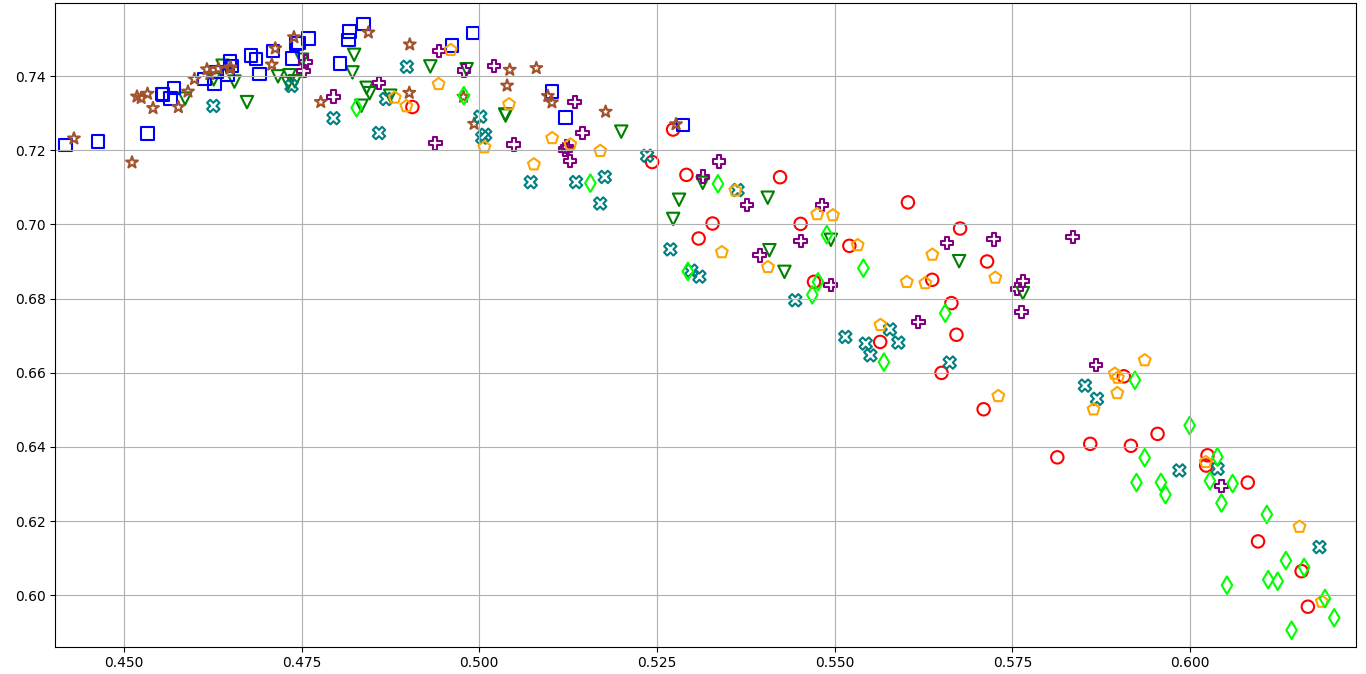
\includegraphics[height=0.35\textheight]{figures/ml2extrasum/lang-basic.png} &
		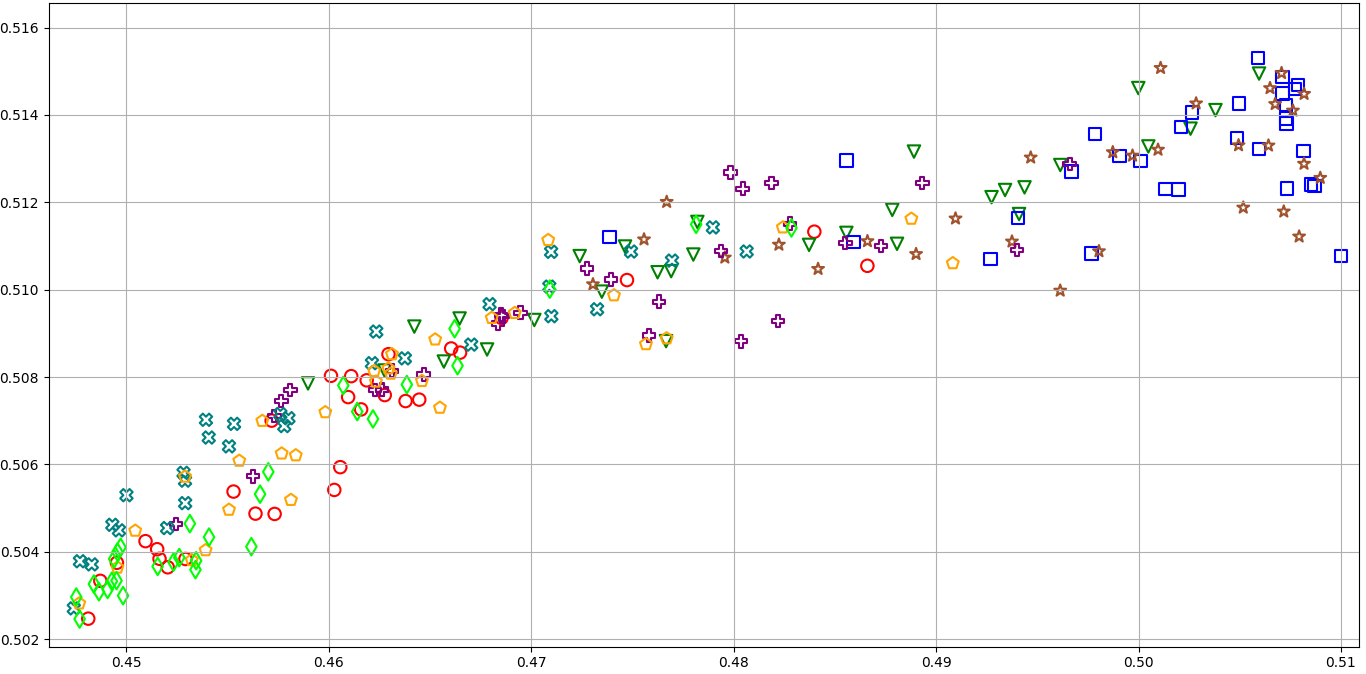
\includegraphics[height=0.35\textheight]{figures/ml2extrasum/lang-filter.png} \\
		(a) using \textit{basic} model & (b) using \textit{filter} model \\
		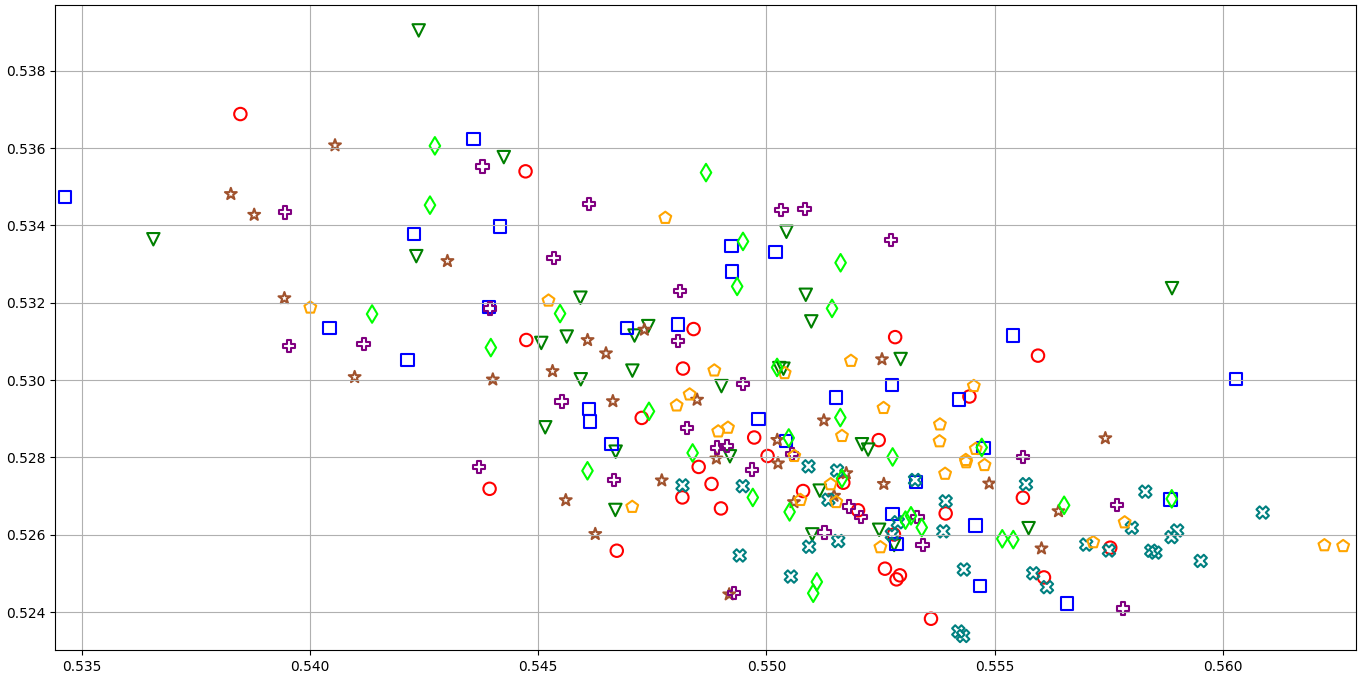
\includegraphics[height=0.35\textheight]{figures/ml2extrasum/lang-norm.png} &
		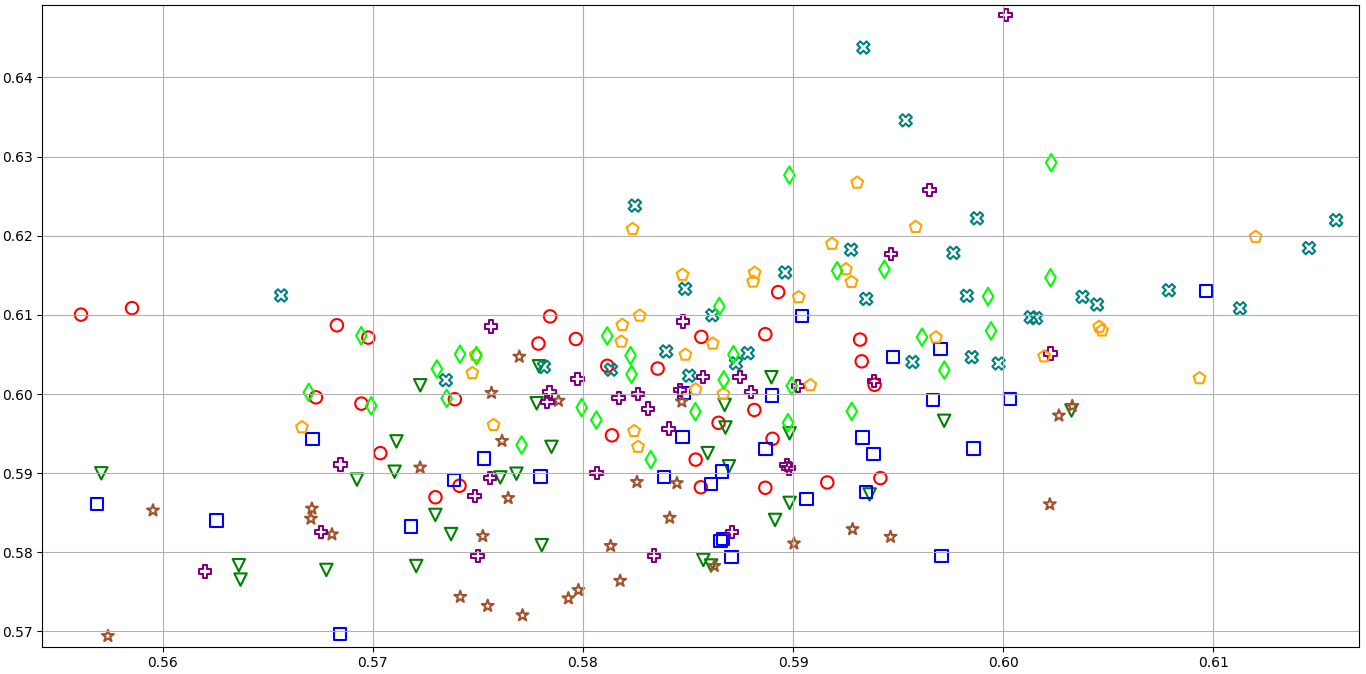
\includegraphics[height=0.35\textheight]{figures/ml2extrasum/lang-pure.png} \\
		(c) using \textit{norm} model & (d) using \textit{pure} model  \\
		\multicolumn{2}{c}{
\includegraphics{figures/ml2extrasum/lang-legend.png}}
	\end{tabular}
	
	\caption{ML2ExtraSum Language scores for 8 languages based on testing corpus using the 4 models.}
	\label{fig:lang-scores}
\end{figure}
\end{landscape}
}

The \textit{basic} model did a good job on clustering the languages, though the interval is too small which is from (0.44, 0.59) to (0.62, 0.75). 
We can see that the two Germanic languages are the most distinct among the others. 
All their documents are situated between (0.41,0.72) and (0.53, 0.76) which is a narrow space compared to others. 
This can tell us that English and Germany may share the same characteristics in term of TF, similarities and sizes. 
Also, it shows that the system learned this information perfectly.
The other languages' documents are not as separable as those of the previous ones. 
Nevertheless, we notice that most documents of each language are situated in the same place: Hebrew to the left; Arabic, French, Japanese and Spanish dispersed in the center; and Chinese which is mostly to the right. 

Filtering the sequences, as shown in Figure~\ref{fig:lang-scores}(b), appears to enhance language clustering. 
It seems that documents of the same language are closer to each other compared to the \textit{basic} model.
This allows us to hypothesize that clustering a document language gives the importance to higher values in our three sequence features.
Nevertheless, the scores' range is too narrow; going from (0.447, 0.502) to (0.51, 0.516). 
Another observation is that the scores using both \textit{basic} and \textit{filter} models are arranged in a linear form rather than spreading over the plane.
This can tell us that using just one dimension is enough to represent the different languages based on these two models. 


Unlike the past two models, normalizing the input values allows the system to represent languages in a two dimensional way as shown in Figure~\ref{fig:lang-scores}(c). 
Except for Spanish and Japanese, it seems that all documents of each language are scattered all around the plane. 
A good clustering would separate each language apart.  
Anyways, just three features is not sufficient to separate as much languages since many languages share the same characteristics. 


Likewise, creating new scalar features before being fed into the system does not do it any favor as shown in Figure~\ref{fig:lang-scores}(d).
The system learns to represent the language in a two dimensional way.
However, these languages are not really separable since most of their documents are swarming into the same place. 
That being said, a given language's documents seem to deviate a little from others of a different language. 
It is not enough to separate them apart, but still promising. 
Maybe, creating more features will help enhancing this task. 


\section{Discussion}

% method description 
We presented an extractive method for multi-lingual text summarization based on machine learning. 
In this method, we use surface statistical features which are weakly dependent on language.
These features can be related to the sentence to be scored or its document; they include: terms frequencies, sentences sizes, sentences similarities, document size and sentences positions. 
The sentence is scored using many scorers: TF scorer, Similarity scorer, Position scorer and Size scorer. 
These scorers use their adequate features beside a score afforded by a language clusterer so they do not score all languages the same. 
The scores afforded by these scorers beside the language clusters are combined using another scorer to afford the final score. 
In our case, this score must be ROUGE-1 score of the sentence in question compared to a reference summary. 
So in summary, the method wants to learn how to estimate ROUGE-1 score of a sentence using some surface features. 
The training uses the actual ROUGE-1 scores; but when trained, the system must estimate what the score will be without referring to any existing summary.


The method was implemented as a system called ``ML2ExtraSum" using neural networks resulting in 4 variants. 
The first variant (\textit{basic}) uses the statistical features as they are without transformation. 
The sequences are fed into an LSTM cell to learn how to reduce their dimension into one or two scalars. 
The second variant (\textit{filter}) is similar to the first, but it filters the sequences by deleting the values under the mean. 
Our assumption is that this will allow the system to focus only on the important values. 
The third variant (\textit{norm}) is similar to the first, but it normalizes the features and filters the sequences before feeding them into the neural network. 
This is done in hope that the normalization will improve the system's performance. 
The fourth variant (\textit{pure}) uses pure scalars as input. 
We generated some new features which are scores in some sort and fed them into the system so it will learn how to combine them into intermediate scores, then a final one. 

To test our system, we used AllSummarizer\_TCC \citep{13-aries-al,15-aries-al}, which does not use machine learning at all, as a baseline system. 
Unfortunately, ML2ExtraSum had no chance against AllSummarizer\_TCC in any of its variants. 
This tells us that our \ac{ml} based architecture maybe needs more than some surface features to reach its full potential. 
Another assumption is that \ac{ml} is not as fit to score the pertinence of a sentence in a multi-lingual context as a traditionally encoded solution based on observation does. 
At least, not in the way our architecture is proposed. 
We must, also, take in consideration that the training batch was a document. 
So, if the whole dataset was used as a batch, result might be different.
Letting the system extracting the features by itself such as using word embedding is interesting, but it will require sacrificing the multi-lingual aspect of the system. 
Moreover, it will consume a lot of data to construct a valid vocabulary. 

%As future directions, we will investigate how adding more features can affect the system's performance.
%Nowadays, there are tools that afford some deep language features for multiple languages, such as BabelNet\footnote{BabelNet website: \url{https://babelnet.org/} [27 August 2019]} \cite{12-naigli-ponzetto}.
%Also, generating more new features may help the system as shown by \textit{pure} model in our experiments. 
%On the bright side, the system shows promising results when it comes to clustering languages based on summarization.
%Same as scoring, the task of clustering  still has to be improved so it can separate languages and represent them in a larger range.






\begin{savequote}[75mm] 
Reasoning draws a conclusion, but does not make the conclusion certain, unless the mind discovers it by the path of experience.
\qauthor{Roger Bacon} 
\end{savequote}

\chapter{General conclusions and discussion}

% problematic 
With the growth of information on the web, it becomes crucial to find ways to process them. 
One way to ease this task is using automatic text summarization. 
\ac{ats} is not a new field, but it is a highly active one due to its importance. 
Finding the perfect formula for \ac{ats} is a challenging task. 
This is because there is no precise definition how should a summary be.
A summary can be good or bad following the opinion of the evaluator; thus the judgment varies from person to person.
But, there are some common criteria to decide if a summary is good enough: informativeness, non redundancy and readability. 
It is necessary that a summary presents most information from the original text. 
Also, a good summary is the one which does not contain redundant information. 
Automatic summaries can be used to enhance other tasks such as indexing. 
But, if the summary is intended as a final result for users, it has to be readable. 
One challenge to achieve a good summarization system is the lack of resources such as toolkits and corpora.

% multilingual ATS
For a long time, English language has been the center of attention by \ac{ats} community. 
But due to the multilingual content increase nowadays, it becomes necessary to develop new tools for other languages. 
There exists some works devoted for languages other than English. 
But due to lack of resources, these works still insufficient for many languages. 
A solution is to design multilingual methods (and systems) which require less language-dependent resources.


% related works chapters summary
A literature review has been presented to introduce \ac{ats} especially in multilingual context. 
First, a concise introduction to the different methods used for \ac{ats} following the taxonomy proposed by \citet{98-hovy-lin,99-sparckjones}. 
We discussed these different methods in term of multilingualism.
Next, different approaches has been presented classifying \ac{ats} methods based on their resources usage. 
We based our taxonomy on the one of \citet{12-lloret-palomar} and \citet{11-nenkova-mckeown}, but with a huge influence of their resources consumption.
Before finishing the literature review, we have discussed \ac{ats} evaluation which is an important topic in this domain.

% contribution chapters summary
After introducing \ac{ats}, a brief description on our participation in MultiLing'15 workshop has been presented. 
We tried to ameliorate our previous work \citep{15-aries-al} by adding multiple languages, using other features than term frequencies, and proposing a new method to extracting the sentences after being scored. 
The extraction method is based on sentences similarities and scores. 
The first sentence to the summary is the highest scored. 
Then, each time we want to add a new sentence, it must have less similarity than a given threshold with the last one added to the summary. 
%chapter contribution
Then, a chapter is reserved for our new method which combines surface features with graphs approach in order to score sentences. 
To score sentences, we construct a graph based on their similarities and we minimize it into a less number of candidate ones. 
Each sentence is scored using surface features, then this score is improved based on the graph. 
To extract the relevant sentences, we proposed some extracting mechanisms based on the graph. 
%chapter machine llearning
After that, we presented a chapter about another method we proposed using machine learning and statistical features to extract sentences. 
The method is based on neural networks by expressing the problem of text summarization as a problem of regression.
It seeks to learn how to estimate ROUGE-1 score based on some statistical features.
Also, it seek it tries to maintain the multilingual aspect by learning how to score the document's language based on the these features.

% Recommendations (implications)
In conclusion, multilingual automatic text summarization is an important domain nowadays.
It can help professionals processing the huge information overload due to the increase rate of multilingual web content.
In this case, the more a system uses language-independent resources, such as toolkits and corpora, the more it can adapt to new languages. 
The method's type used to implement such system is crucial to decide how multilingual this system can be. 
Lets take abstractive summarization as an example; it is very difficult to implement an abstractive multilingual \ac{ats}. 
So, it is more simple to use an extractive method.
That being said, a fully multilingual system is no use if it does not afford informative summaries.
The whole idea of summarization is to preserve the most relevant information from the original text in a compact form.
This leads us to think about redundancy; a summary with less redundancy is better. 
In fact, if we look at summarization from this view point, summaries are mostly used to decrease redundant information in huge content.
Another criterion to judge the quality of a summary is readability which encompasses reference clarity and coherence. 
Most works do not give more important to this one because summaries are usually used to enhance some other automatic tasks; they are not intended for humans. 
But, it stills a good thing to find a multilingual way to enhance summaries readability.


\section{Contributions}

% Informativeness 
Informativeness is the most important indicator of a good summary.
In this thesis, we tried to maximize the quantity of information a summary can contain whatever the language of the original text. 
First of all, we enhanced our previous method (TCC) \citep{13-aries-al} and tested it in a multilingual context by participating in MultiLing'15 workshop \citep{15-aries-al}.
The method, being tested and proved its quality, has been used as a baseline to test our new method (SSF-GC). 
The new method called ``Sentence statistical features, Graph-based cumulative scores" (SSF-GC) combines surface features and similarity graph to score sentences, as indicated by its name. 
The graph is used to exclude some sentences which have week links with others, thus they are off-topic and less informative. 
We can consider this step as a noise removal task to enhance the scoring function. 
The informativeness of each sentence is expressed as its probability to belonging to the summary based on some statistical features. 
In our case, this probability is affected by the sentence's neighbors' in the graph using accumulation.
We proposed some scoring functions which gave good results.
Our machine learning based method (ML2ExtraSum) could not beat TCC method in term of informativeness. 
Nevertheless, it affords close results and it can be a good start to be enhanced in the future.


% Redundancy 
Redundancy is another issue in \ac{ats}. 
Unlike MMR \citep{98-carbonell-goldstein} which tries to handle informativeness and redundancy using one score, we treat redundancy while extracting sentences. 
This separation gives us more freedom on how we extract relevant sentences based on their informativeness scores, but using some conditions to decide if the summary has already the information in a sentence about to be extracted. 
A first attempt was to use similarity between the last sentence added to the summary and the next one being considered for the summary. 
If there is a huge similarity between them, we consider another sentence. 
This extraction method has proven to be a good one. 
It does not just improve non redundancy, but also informativeness by letting the space for more new information. 
We tested using other variants, mostly based on the graph. 
One variant, in particular, gives good results. 
It is similar to the one we described earlier, but it is based on the graph. 
First, we choose the highest scored sentence among the candidates. 
Then, out of its neighbors, we choose the one which maximizes the score and minimizes the similarity.  

% Coherence
Also, we tried to propose some extraction methods with coherence in mind. 
Mostly, a paragraph's sentences have some shared terms, especially the consecutive one. 
So, when we order sentences, it is natural that a sentence following another has some similarity. 
But, this similarity must not exceed some limit, otherwise it will be a repetition. 
Unfortunately, we did not test how far this assumption is true, and how to define such limit.

% delivrables 
Aside from the theoretical contributions, this thesis contributes to the state of art by making tools available to the community. 
We designed some open source tools to support this thesis; the most important are these two which we talked about earlier in this thesis:
\begin{itemize}
	\item \textbf{AllSummarizer}: A Java platform for extractive text summarization. 
	It implements the two methods discussed here, in this thesis \citep{13-aries-al,15-aries-al,18-aries-al,21-aries-al}.
	It has three parts: preprocessing, processing and postprocessing. 
	More information about the system is presented in Appendix A.
	
	\item \textbf{LangPi}: a Java tool for preprocessing: Normalization, Segmentation, Stemming and Stop words removal.
	The tool affords ROUGE metrics for summarization which support multilingual evaluation. 
	
	\item \textbf{ML2ExtraSum}: a Python tool for extractive text summarization based on machine learning using Tensoflow. 
	Along with it, a preprocessed corpus based on MultiLing'15 MSS corpus.
	
\end{itemize}


\section{Limits}

% simplicity
In our work, we tried to propose a method for multilingual \ac{ats} which is simple yet effective.
In the end, simple things are not always bad;  like Leonardo da Vinci said: ``Simplicity is the ultimate sophistication.".
However, usually complex tasks such as \ac{ats} demand complex mechanisms. 
In \ac{ssf-gc} method, we assumed the different features scores are probabilities and combined them accordingly.
This assumption gave good results, yet it does not mean there are no better combinations. 
Although we had to avoid machine learning due to language dependency, we decided to test using this approach in our method/system ML2ExtraSum. 
So, we formulated summarization task as a regression problem: estimating ROUGE-1 score from a set of features. 
The scoring function is estimated using many neural networks blocks: Language Clustering Scorer, TF-ISF Scorer, Similarity Scorer, Size Scorer and Position Scorer. 
Each of these blocks affords a score, then all these scores are fed to another block called ``Sentence Scorer" to estimate ROUGE-1 score of the sentence.
The system was trained using Multling'15 MSS training corpus and tested using the testing one. 
Unfortunately, this method did not outperform our \ac{tcc} method, because the system could not estimate ROUGE-1 properly. 
%A more detailed description of this experience can be found in Appendix B.

% pertinence and redundancy
Like we said, a task such as \ac{ats} is way too complex to be expressed by a simple method. 
Surface features are good indicators on a sentence's pertinence. 
Nevertheless, they cannot express the deep meaning of sentences. 
As a consequence, a sentence can be pertinent to the general topic but the system cannot capture that; for example, if it contains synonyms of important terms.
Also, the final summary can have redundant sentences, which does not share the same terms but have the same meaning.


%% readability
Readability remains an issue of \ac{ats}. 
In our case, we tried to focus on coherence using sentences ordering. 
Unfortunately, this was not tested since it needs a lot of experts to access the order of sentences. 
Also, anaphora resolution and replacing conjunctions were not treated in our work since these operations can be seen as a post-processing task.


\section{Future works}

% talk about 
Our SSF-GC method affords acceptable results in the context of multilingual \ac{ats}, given the tests we performed.
However, looking at the limits we enlisted earlier, it is still far away from being a perfect one. 
Statistical surface features are good indicators of sentence pertinence.
Therefore, they afford good summaries in term of informativeness, without sacrificing the method's multilingualism.
Still, they cannot capture the whole meaning, which results in less informativeness and more redundancy. 
In this case, a more sophisticated approach is to summarize ideas in a language-independent format. 
To do this, we have to design a way to represent sentences in a general way without loosing their meanings.
This leads us to Chomsky's universal grammar which states that there is an innate language faculty, which is genetically determined, that allows children to learn a specific language \citep{80-chomsky}.
We will not discuss language acquisition theories and nativism theory criticism (although, there are neuroscience researches suggesting Chomsky may be right \citep{16-ding-al}). 
The objective is to find a representation which can satisfy a maximum number of languages, even if there are some exceptions.


If we can find a way to represent sentences meanings regardless their original language, it is not just multilingual \ac{ats} that will be improved. 
We can talk about cross-lingual summarization, which seeks to generate a summary in a language different from the original one. 
We can go further by summarizing multiple documents in many different languages into a summary with a target language.
That being said, this is not possible unless we have some language-dependent tools. 
A universal representation of the meaning can help us create multilingual methods for \ac{ats}. 
However, we have to possess the tools allowing us to pass from each natural language to this representation and vice versa. 
In the end, the problem of multilingual \ac{ats} comes back to resources' availability.


Another alternative is to exploit machine learning while trying to maintain the system's independence from the training corpus. 
To this end, we implemented a multilingual system (ML2ExtraSum) based on machine learning; but it could not surpass the baseline.
As future directions, how adding more features can affect the system's performance must be investigated.
Nowadays, there are tools that afford some deep language features for multiple languages, such as BabelNet\footnote{BabelNet website: \url{https://babelnet.org/} [27 August 2019]} \citep{12-naigli-ponzetto}.
Also, generating more new features may help the system as shown by \textit{pure} model in our experiments. 
On the bright side, the system shows promising results when it comes to clustering languages based on summarization.
Same as scoring, the task of clustering  still has to be improved so it can separate languages and represent them in a larger range.

%\singlespacing

% the back matter
\clearpage

\begin{spacing}{1}
	{\footnotesize \bibliography{references}}
	\addcontentsline{toc}{chapter}{References}
\end{spacing}

\appendix
\captionsetup{list=no}
\setcounter{tocdepth}{0}
%\settocdepth{chapter}

%\begin{appendix}

\chapter{Tools: A technical report}

In this report, we will present the technical aspect of our thesis. 
We will present the tools developed during this thesis, namely LangPi and AllSummarizer. 
AllSummarizer is intended to be an extractive text summarization system, which affords two methods: \ac{tcc} \citep{13-aries-al,15-aries-al} and \ac{ssf-gc} \citep{18-aries-al,21-aries-al}.
\ac{tcc} method uses clustering to group similar sentences (finding topics), then it uses some statistical surface features with Bayes classification to estimate the sentences which can represent the most topics. 
\ac{ssf-gc} method uses the same statistical features to score sentences, then a graph of similarity is used to enhance this score.
LangPi was created to separate preprocessing tasks from AllSummarizer and enable adding new languages as plugins. 

 
\section{LangPi overview}

LangPi (Language Processing Interface) is a toolkit which we developed in order to afford some tools for processing different natural languages. 
Mainly, it focuses on preprocessing task which is used mostly in \ac{ir} systems. 
Table~\ref{tab:langpi-tech} represents technical information about LangPi. 

\begin{table}[!ht]
	\centering
	\caption{Technical information about LangPi}
	\readtable{technical/langpi-tech.tex}
	\label{tab:langpi-tech}
\end{table}


\subsection{Package: basic} 

This package affords basic languages processing tasks represented in Table~\ref{tab:basic-tasks}.
Each language must implement this interface to afford these functionalities.

\begin{table}[!ht]
	\centering
	\caption{Basic tasks in LangPi toolkit}
	\readtable{technical/basic-tasks.tex}
	\label{tab:basic-tasks}
\end{table}


\subsubsection{Normalization}

%Church, K.: One Term or Two? In: Proceedings of SIGIR 1995, pp. 310–318 (1995)
Normalization is the process of transforming a document to a standard more easy to manipulate format. 
In case of multi-document summarization, different documents may have the same word with different writing forms. 
For instance, a document can contain all these words which are the same: ``Mr.", ``mister" and ``Mister".
Here are some operations that can be used in this task:
\begin{itemize}
	\item Special characters removal. For example, if the system does not need separated paragraphs, we can delete new lines character. 
	\item Numbers transformation from numerical to letters (pronunciation) or the inverse. If the numbers information is not important to the task, it can be deleted.
	\item Equivalent words replacement such as abbreviations or words used in chat.
	\item Diacritical marks removing, such as replacing ``résumé" with ``resume" in French.
	\item Styling text suppression, such as HTML markers.
\end{itemize}

LangPi affords un \ac{api} which can be implemented for each language. 
The \ac{api} description is presented in Table~\ref{tab:normalizer-api}.
It is implemented by 29 languages (plus a default one) where the main function is just to delete new lines and multiple spaces. 
In Arabic, it deletes diacritics as well.
\begin{table}[!ht]
	\centering
	\caption{LangPi Normalizer \ac{api}}
	\readtable{technical/normalizer-api.tex}
	\label{tab:normalizer-api}
\end{table}


\subsubsection{Segmentation}

% sentence segmentation challenges
Segmenting a text refers to two tasks: sentence boundary detection and tokenization. 
In many languages, a sentence is ended by either a dot, a question mark or an exclamation mark. 
This is not the case for all languages, such as Thai which does not have a delimitation mark for sentences. 
Even using a full stop as a delimiter, abbreviations such as ``Mr.", ``Dr." and ``etc." when they occur in the middle of a sentence can be problematic. 
Also, other punctuation marks can be used to separate sentences \citep{10-palmer}, such as commas used to express actions sequence.

To perform sentence segmentation, regular expression with a list of abbreviations \citep{89-riley,97-reynar-ratnaparkhi} and proper nouns \citep{02-mikheev} can be used. 
Many regular expressions can be defined to detect cases where a dot can occur such as the dot in numbers.
More features can be used to enhance this task; they can be used together with machine learning to estimate the probability of a dot being a sentence boundary. 
Here a list of features used especially for English texts:
\begin{itemize}
	\item Letter's case: sentences start with uppercase letters.
	\item Part of speech (PoS): \citet{97-palmer-hearst} use parts of speech with machine learning to enhance sentence boundary detection.
	\item Word's size: this feature is used in \citep{89-riley} on the two words before and after the dot.
	\item Prefixes and suffixes: They are used to enhance boundary detection since abbreviations does not have suffixes \citep{80-muller-al,97-reynar-ratnaparkhi}.
\end{itemize}


Another type of segmentation is word tokenization which can be performed by breaking the text into words using the space (blank mark).
But, it is not as easy as that, since there are many challenges:
\begin{itemize}

	\item Punctuation marks are taken as separate tokens. But in case of abbreviations, the dot must not be separated from the word before.
	
	\item Some marks, such as the apostrophe, have many functions. 
	In English, the apostrophe can be used as citation mark, it can be used in possessive form (\textit{Karim's thesis}), or it can be used as a contraction (\textit{I'm}). 
	In French, the apostrophe is used for contraction as well (\textit{l'homme}, \textit{j'ai}, \textit{qu'ils}, etc.).
	
	\item Some languages use composed words either by joining them directly or using the hyphen. 
	In German, it is so common to use words composition such as noun-noun (\textit{Lebensversicherung}: life insurance).
	In Arabic, some prepositions and determiners are attached to the word (\textarab{ويساعدهم} /wa-yus\={a}`ida-hum/: and he helps them).
	Sometimes words with attached prepositions can be confused with words, for example the expression (\textarab{وعود} /wa-`\={u}d/: and Oud) can be confused with the word (\textarab{وعود} /wu`\={u}d/: promises).
	Other languages use hyphens, such as English (\textit{end-of-file}, \textit{classification-based}, etc.) and French (\textit{va-t-il}, \textit{c'est-à-dire}, \textit{celui-ci}, etc.). 
	
	\item There exists some languages without words boundaries, such as Chinese, Japanese and Thai. 
	For example, reading this sentence (このきれいな写真はどこに取りましたか。 \textit{/kono kirei-na shashin wa doko ni torimashika ka./}: Where did you take this beautiful picture.), someone who knows Japanese can separate the different words, yet it is difficult to separate them automatically.
	
	%
\end{itemize}

The Segmenter's \ac{api} description is presented in Table~\ref{tab:segmenter-api}.
It contains two public methods: one for segmenting a text into sentences and te other to segment a text (a sentence) into words.
\begin{table}[!ht]
	\centering
	\caption{LangPi Segmenter \ac{api}}
	\readtable{technical/segmenter-api.tex}
	\label{tab:segmenter-api}
\end{table}

As for the implementation, we use open source tools when they are available;
Otherwise, we use regular expressions (Regex).
Table~\ref{tab:segmenter-tools} shows the tools used to implement segmentation for each supported language.
For Thai, the resources work just on OpenNLP 1.4; they are not compatible with ulterior versions. 
So, we modified OpenNLP 1.4 code by renaming its namespaces, so it will not clash with ulterior versions.
\begin{table}[!ht]
	\centering
	\caption{LangPi Segmenter tools}
	\readtable{technical/segmenter-tools.tex}
	\label{tab:segmenter-tools}
\end{table}

\subsubsection{Stemming}

When we count the frequency of terms in a document, many words can occur in different forms due to conjugation and inflection. 
These morphological variations represents the same meaning and must be treated as such. 
This is why we need to remove  prefixes, suffixes and infixes from words before processing them. 
This operation is called ``Stemming", which reduces words to a certain form called ``stem" and can be considered as a normalization function.
A stem can be a word without meaning, for example the stem ``condit" from the word ``conditional".
The benefit of Stemming is not just having a unified form for the different words in the text.
But, also, it serves as a mean to reduce the vocabulary resulting in less memory usage and fast processing.  
The most known approach for stemming is Porter \citep{97-porter} which affords some rules to slice the prefixes and suffixes in a certain order. 
Like Stemming, Lemmatization is the process of finding a standard form called ``lemma" which is a dictionary word. 
For example, the word ``would" stays as it is after stemming, while after lemmatizing we get ``will".

The Stemming \ac{api} of LangPi contains one method (See Table~\ref{tab:stemmer-api}.
It is important to point out that we do not make a difference between stemming and lemmatizing. 
\begin{table}[!ht]
	\centering
	\caption{LangPi Stemmer \ac{api}}
	\readtable{technical/stemmer-api.tex}
	\label{tab:stemmer-api}
\end{table}

To implement stemming task, we used the tool illustrated in Table~\ref{tab:stemmer-tools}.
\begin{table}[!ht]
	\centering
	\caption{LangPi Stemmer tools}
	\readtable{technical/stemmer-tools.tex}
	\label{tab:stemmer-tools}
\end{table}


\subsubsection{Stop-words elimination}

Some words such as articles, pronouns, conjunctions, etc. are common in a text, yet they do not contribute so much in the subject of this text. 
This is why some \ac{ir} systems ignore them allowing more space in the database. 
Some systems avoid ignoring stop-words to support phrasal search. 
In conclusion, this task can be beneficial or not according to what we are looking to do. 
For instance, if we are working on a system  based on language understanding, it is better not to remove stop-words. 
Otherwise, the system will not be able to process the text correctly, such as distinguishing between affirmative and negative forms using ``not". 
Some other systems, such as statistical text summarizers, are more comfortable with removing them. 


The Stop-words eliminator \ac{api} of LangPi contains one method which takes a list of words and remove stop-words from it (See Table~\ref{tab:swe-api}. 
The languages having stop-words are: Arabic, Chinese, Czech, Dutch, English, Finnish, French, German, Greek, Hindi, Hungarian, Italian, Norwegian, Portuguese, Romanian, Russian, Spanish, Swedish, Turkish
\begin{table}[!ht]
	\centering
	\caption{LangPi Stop-Words Eliminator \ac{api}}
	\readtable{technical/swe-api.tex}
	\label{tab:swe-api}
\end{table}


\subsection{Package: eval}

This package is primarily created to evaluate automatic text summarization. 
It seeks to re-implement \ac{rouge} toolkit, which is written in Perl, and exploit the preprocessing \ac{api} to afford multilingual evaluation. 
In this version (1.1.5), just ROUGE-1 and ROUGE-2, which are too used in evaluation camps, are implemented.
Figure~\ref{fig:langpi-eval} represents class diagram of package ``kariminf.langpi.eval.ats".
%
\begin{figure}[!ht]
	\begin{center}
		\includegraphics[width=.8\textwidth]{figures/technical/langpi-eval.pdf}
	\end{center}
	\caption{\label{fig:langpi-eval} Class diagram of the package ``kariminf.langpi.eval.ats"}
\end{figure}

This tool can be used by instantiating the class ``KRouge". 
To understand how to use it, there is no better way than a little tutorial. 
First of all, the class must be imported as follows 

\begin{lstlisting}[language={Java}, style=codeStyle] 

import kariminf.langpi.eval.ats.KRouge;

\end{lstlisting}

For the sake of the tutorial, lets say we have one peer (system's summary) and two models (reference summaries). 
First, we create some fake sentences to test our program.
In real application, the sentences are created by using the preprocessing package presented earlier. 

\begin{lstlisting}[language={Java}, style=codeStyle]

List<List<String>> peer1 = new ArrayList<>();
peer1.add(Arrays.asList(new String[]{"a", "f", "b", "e", "b", "e"}));
peer1.add(Arrays.asList(new String[]{"a", "f", "d", "e"}));

List<List<List<String>>> models = new ArrayList<>();

List<List<String>> modelTmp = new ArrayList<>();
modelTmp.add(Arrays.asList(new String[]{"a", "a", "b", "c", "b", "d"}));
modelTmp.add(Arrays.asList(new String[]{"b", "c", "d"}));
models.add(modelTmp);

modelTmp = new ArrayList<>();
modelTmp.add(Arrays.asList(new String[]{"a", "a", "b", "c", "b", "d", "a", "b"}));
models.add(modelTmp);

\end{lstlisting}

We instantiate the class ``KRouge" by affording the type of \ac{rouge}.
Then, for each new model, we afford the sentences tokenized into words. 
The same thing is applied to the peer which we want to evaluate.

\begin{lstlisting}[language={Java}, style=codeStyle]

for(List<List<String>> model: models){
	//call this each time you want to create a new model
	evaluator.newModel();
	//charge the current model's sentences
	for (List<String> sent: model) evaluator.addModelSentence(sent);
}

for (List<String> sent: peer1) evaluator.addPeerSentence(sent);
\end{lstlisting}

Finally, we calculate the metrics and print the result. 
If we want to evaluate another peer with the same models, there is no need to load models again. 
There is a method which clears just the peer's sentences.

\begin{lstlisting}[language={Java}, style=codeStyle]

evaluator.calculate();

System.out.println("The recall is: " + evaluator.getRecall());

//If you want to use the same models with a new peer, use this method
evaluator.resetPeer();
\end{lstlisting}


\subsection{Package: wordnet}

This package is intended as an easy to use interface for browsing Wordnet \citep{95-miller} which is a a lexical database for the English language.
It affords a class to access an SqlLite database containing multilingual Wordnets, which we assembled from ``Open Multilingual Wordnet" project\footnote{Open Multilingual Wordnet: \url{http://compling.hss.ntu.edu.sg/omw/} [15 August 2019]}.
This package is intended to be used in future research. 
Figure~\ref{fig:langpi-wordnet} represents class diagram of this package.

\begin{figure}[!ht]
	\begin{center}
		\includegraphics[width=.8\textwidth]{figures/technical/langpi-wordnet.pdf}
	\end{center}
	\caption{\label{fig:langpi-wordnet} Class diagram of the package ``kariminf.langpi.wordnet"}
\end{figure}

\subsection{How to use}

The packages are deployed on JitPack (see Table~{tab:langpi-tech}), which helps deploying a package directly from Github. 
It supports many build automation systems: gradle, maven, sbt and leiningen. 
We will focus on Gradle in the following tutorial. 
So, first of all, you have to add JitPack repository to your root \textbf{build.gradle}:

\begin{lstlisting}[style=codeStyle] %language={[KB]Javascript}, 

   repositories {
      ...
      maven { url 'https://jitpack.io' }
   }
\end{lstlisting}

Then, you add the dependency if you want to use the whole project.

\begin{lstlisting}[style=codeStyle] %language={[KB]Javascript}

   dependencies {
      compile 'com.github.kariminf:langpi:1.1.5'
   }
\end{lstlisting}

In case you want to use just some packages of the project, we afford that as well. 
As you can see, there are two packages for ``basic": one with the usual license (Apache-2) and the other is licensed under AGPL-3. 
The latter contains Hebrew and Thai which use some GPLed software preventing us from distributing it under Apache-2 license. 

\begin{lstlisting}[style=codeStyle] %language={[KB]Javascript}

   dependencies {
      compile 'com.github.kariminf.LangPi:langpi-basic-agpl3:1.1.5'
      compile 'com.github.kariminf.LangPi:langpi-basic-main:1.1.5'
      compile 'com.github.kariminf.LangPi:langpi-eval:1.1.5'
      compile 'com.github.kariminf.LangPi:langpi-wordnet:1.1.5'
   }
\end{lstlisting}


\section{AllSummarizer overview}

AllSummmarizer is an open source statistical \ac{ats} system written in Java and released under Appache 2.0 license. 
It was developed in the context of Magister diploma \citep{13-aries-al}, and first deployed on Github in May 25th, 2013.
This version was ameliorated by adding more languages, fixing bugs, adding more features and supporting a more modular architecture \citep{15-aries-al}.
Then, the system was enriched by some other packages: ssfgc, eval \citep{18-aries-al} and wordnet.


Figure~\ref{fig:as-packages} shows the general architecture of AllSummarizer system as a package diagram.
In this diagram, just the important parts of the system as presented: tools, preprocess, process and postprocess. 
To summarize a text, it passes by preprocessing where it is segmented into sentences and words, filtered from unwanted words and normalized. 
This is the language-dependent part of the system, which uses the previously described project: LanPi. 
The preprocessed text is stored in a ``Data" to be treated by the next step. 
Then, the processing part is where the importance of each sentence is decided based on some statistical features. 
Currently, there are two methods: \acl{tcc} and \acl{ssf-gc}. 
Finally, the text is postprocessed using the scores to extract relevant sentences.   

\begin{figure}[!ht]
	\begin{center}
		\includegraphics[width=\textwidth]{figures/technical/as-packages.pdf}
	\end{center}
	\caption{\label{fig:as-packages} Package diagram of AllSummarizer}
\end{figure}


\subsection{Package: tools}

This package contains two helping classes: ``Data" and ``Tools". 
``Data" class is intended to be a container which transports information between tasks; mostly preprocessing task.
It affords some methods to store and retrieve information, mostly for preprocessing task.
``Data" \ac{api} description is presented in Table~\ref{tab:data-api}.
\begin{table}[!ht]
	\centering
	\caption{AllSummarizer preprocess.tools.Data \ac{api}}
	\readtable{technical/data-api.tex}
	\label{tab:data-api}
\end{table}


``Tools" class affords some static methods used to calculate cosine similarity, words frequencies in both sentences and documents, statistics about terms, etc.
It is used mostly by ``Data" class.


\subsection{Package: preprocess}

This package affords just one interface specifying functions to setting a ``Data" object in which the result of preprocessing will be stored, adding one or multiple texts and starting the preprocesssing.
To preprocess te texts, it uses LangPi ``basic" package's \ac{api}: Normalizer, Segmenter, Stemmer and SWEliminator.
Two implementations are afforded: the static one links Allsummarizer to LangPi directly and the dynamic one is used in case someone wants to add new languages. 
The dynamic class searches for packages in a specific folder (by default ``preProcess"), which must implement the LangPi ``basic" \ac{api}.
Figure~\ref{fig:as-preprocess} represents class diagram for ``preprocess" package.

\begin{figure}[!ht]
	\begin{center}
		\includegraphics[width=.7\textwidth]{figures/technical/as-preprocess.pdf}
	\end{center}
	\caption{\label{fig:as-preprocess} Class diagram of the package ``kariminf.as.preprocess"}
\end{figure}


The following code is an example on how to preprocess an English text. 
The ``Data" object is used to store the result of the preprocessing, so it must be set before calling the ``preProcess" method.
The method ``addText" is used to add a document at once. 
So, if we have multiple documents, we call it multiple times. 

\begin{lstlisting}[language={Java}, style=codeStyle]
import java.util.List;
import kariminf.as.preProcess.PreProcessor;
import kariminf.as.preProcess.StaticPreProcessor;
import kariminf.as.tools.Data;

public class TestPreProcess {

    public static void main(String[] args) {

        String text = ""; //put a text here
        Data data = new Data();
        PreProcessor prep = new StaticPreProcessor("en");
        prep.setData(data);
        prep.addText(text);
        prep.preProcess();

        //retrieve some information from data
        List<String> sentences = data.getSentences();
        List<List<String>> sentWords = data.getSentWords();
        List<List<Double>> sim = data.getSentSimilarities();

    }
}

\end{lstlisting}

\subsection{Package: process}

This package is the core of the program; its job is to score sentences based on some criteria. 
Figure~\ref{fig:as-process} represents the class diagram of this package. 
It affords a class (``Scorer") which retrieves sentences' features from a ``Data" object, scores them and affords their scores and orders of pertinence. 
In order for this class to score a given sentence (by its number), the method ``scoreUnit" afforded by the interface ``ScoreHandler" is used.
This interface can be implemented to afford different ways of scoring. 
In this version (1.1.5), two scoring methods are implemented represented by two packages:
\begin{itemize}
	\item \textbf{tcc}: it stands for \acl{tcc}.
	This packages includes ``Clusterer", NaiveCluster", ``BayesScoreHandler", "Features" and its implementations. 
	The method clusters similar sentences together, trains a naive Bayes classifier on these clusters based on some features, then scores each sentence by calculating the probability of it representing all of these clusters. 
	\item \textbf{ssfgc}: it stands for \acl{ssf-gc}. 
	This package includes ``SSFScoreHandler" and its subclasses. 
	The method constructs a graph based on sentences' similarities, reduces the graph to obtain some candidate sentences, scores each sentence based on statistical features and then improves these scores using the graph structure.
\end{itemize}

\begin{figure}[!ht]
	\begin{center}
		\includegraphics[width=\textwidth]{figures/technical/as-process.pdf}
	\end{center}
	\caption{\label{fig:as-process} Class diagram of the package ``kariminf.as.process"}
\end{figure}

\subsubsection{Package: process.tcc}

In this package, ``ScoreHandler" is implemented by the class ``BayesScoreHandler" which uses two elements: ``Clusterer" and "Feature". 
The idea of this method can be summarized into these points:
\begin{enumerate}
	\item First, it looks for different topics using clustering, taking in consideration that a sentence can belong to many topics. 
	The abstract class ``Clusterer" affords a mean to implement different methods for clustering by extending the abstract method ``createClasses". 
	Currently, the only implementation is ``NaiveCluster" which uses cosine similarity and a threshold to judge if two sentences are similar or not. 
	If they are, then they share the same topic and hence must belong to the same cluster. 
	
	\item Then, ``BayesScoreHandler" scores each sentence by estimating the probability that it belongs to a topic using Bayes classifier. 
	A classifier feature is represented by the interface ``Feature", which is implemented by some classes: TFU, TFB, Pos, PLeng and RLeng.
	
\end{enumerate}
For more information about the theory behind this method, you can check Chapter~\ref{chap:tcc} or these papers: \citep{13-aries-al,15-aries-al}.


Here is a piece of code on how to use this package. 
The preprocessing code is omitted and can be found in preprocess package's section.  
\begin{lstlisting}[language={Java}, style=codeStyle]
import java.util.List;
import kariminf.as.process.Scorer;
import kariminf.as.process.tcc.BayesScoreHandler;
import kariminf.as.process.tcc.NaiveCluster;
import kariminf.as.process.tcc.Pos;
import kariminf.as.process.tcc.TFB;
import kariminf.as.tools.Data;

public class TestTCC {

    public static void main(String[] args) {
    
        Data data = new Data();
        //... preprocessing phase

        NaiveCluster nc = new NaiveCluster(0.25);
        BayesScoreHandler bsh = new BayesScoreHandler(nc);
        Scorer s = Scorer.create(bsh);
        s.setData(data);//calls bsh.setData(data)

        bsh.addFeature(new TFB());//calls TFB.setData(data);
        bsh.addFeature(new Pos());//calls Pos.setData(data)


        bsh.train();//must train before scoring
        s.scoreUnits();//calls bsh.scoreUnit(i);

        List<Integer> order = s.getOrdered();
        double sent1score = s.getScore(1);//sentence 1 score
    }
}

\end{lstlisting}

\subsubsection{Package: process.ssfgc}

In this package, ``ScoreHandler" is implemented by the class ``SSFScoreHandler" which constructs a graph of similarities, reduces the graph to have candidate sentences, then scores these sentences using some statistical features. 
This class is extended by 5 subclasses to improve the statistical scores based on the graph structure:
\begin{itemize}
	\item \textbf{GC0ScoreHandler}: this class does not improve the scores based on graph; it just return the same scores as ``SSFScoreHandler". 
	It is used as a baseline to show how the graph improves the scoring function.
	
	\item \textbf{GC1ScoreHandler}: this class adds to each node's score (sentence) the scores of its neighbors in the graph weighted by their similarities.
	
	\item \textbf{GC2ScoreHandler}: this class adds to each node's score (sentence) the scores of its neighbors in the graph and subtracts the scores of non neighbors.
	
	\item \textbf{GC3ScoreHandler}: this class amplifies each node's score (sentence) by the number of its neighbors plus one.
	
	\item \textbf{GC4ScoreHandler}: this class multiplies each node's score (sentence) by the sum of its similarities with its neighbors. 
	
\end{itemize}
For more information about the theory behind this method, you can check Chapter~\ref{chap:gc} or these papers: \citep{18-aries-al,21-aries-al}.

Here is a piece of code on how to use this package. 
The preprocessing code is omitted and can be found in preprocess package's section.  
\begin{lstlisting}[language={Java}, style=codeStyle]
import java.util.List;
import kariminf.as.process.Scorer;
import kariminf.as.process.ssfgc.GC1ScoreHandler;
import kariminf.as.process.ssfgc.SSFScoreHandler;
import kariminf.as.tools.Data;

public class TestSSFGC {

    public static void main(String[] args) {

        Data data = new Data();
        //... preprocessing phase

        SSFScoreHandler ssh = new GC1ScoreHandler(0.1);//similarity threshold = 0.1
        Scorer s = Scorer.create(ssh);

        s.setData(data);//calls ssh.setData();
        ssh.calculateSSFScores();//must calculate ssf scores before scoring
        s.scoreUnits();//calls bsh. scoreUnit (i);

        List<Integer> order = s.getOrdered();
        double sent1score = s.getScore(1);//sentence 1 score
    }
}

\end{lstlisting}

\subsection{Package: postprocess}

Scoring relevant sentences is not enough to construct a summary. 
When the scoring function does not take into consideration redundancy, this latter must be treated while extracting sentences. 
Also, sentences order is important for readability since te sentences are extracted from different parts of the text. 
Sometimes, some sentences contain broken references such as personal pronouns which have to be replaced. 
Figure~\ref{fig:as-postprocess} represents class diagram of the postprocessing task in AllSummarizer. 
The ``PostProcessor" class defines the abstract method ``postProcess" which triggers the task. 
Allsummarizer in its current version (3.0.1) focuses on extraction based on the scores.
the class ``Extractor" re-orders te sentences according to their scores and some other criteria (see Chapter~\ref{gc}). 
This class is extended by six classes, two of them are ``SimpleReOrder" and ``ThresholdReOrderer".
``SimpleReOrder" (e0) returns the order based on the scores afforded by the scorer, hence the name \textbf{simple}. 
``ThresholdReOrderer" (e1) uses the scores to reorder the sentences besides a similarity threshold used to exclude similar sentences; so it takes redundancy in consideration.
The 4 remaining extraction methods are based on the graph and they need the scoreHandler to be of type ``SSFScoreHandler".  
In all of these algorithms, the highest scored sentence is added to the summary.
\begin{itemize}
	\item \textbf{GraphReOrderer} (e2) tries exploiting graph structure to ensure coherence between extracted sentences.
	The next sentence to extract must be the highest scored one among the neighbors of the last added one.
	
	\item \textbf{SimNeighborReOrderer} (e3) tries to select the next sentence as the one with a high score and high similarity among the neighbors of the last added one. 
	
	\item \textbf{DiffNeighborReOrderer} (e4) tries to select the next sentence as the one with a high score and lower similarity among the neighbors of the last added one. 
	
	\item \textbf{Neighbors2ReOrderer} (e5) tries to keep the highest scored sentences among the neighbors which have a high amount of non-summary neighbors. 
\end{itemize}

\begin{figure}[!ht]
	\begin{center}
		\includegraphics[width=.7\textwidth]{figures/technical/as-postprocess.pdf}
	\end{center}
	\caption{\label{fig:as-postprocess} Class diagram of the package ``kariminf.as.postprocess"}
\end{figure}

Here is a piece of code on how to use this package. 
The preprocessing and processing code are omitted and can be found in process package's section.  
\begin{lstlisting}[language={Java}, style=codeStyle]
import kariminf.as.tools.Data;
import java.util.List;
import kariminf.as.postProcess.extraction.Extractor;
import kariminf.as.postProcess.extraction.ThresholdReOrderer;
import kariminf.as.process.Scorer;

public class TestSSFGC {

    final static int summarySize = 2;

    public static void main(String[] args) {

        //... preprocessing phase
        //Scorer s = ...
        //... processing phase
        
        Extractor e = new ThresholdReOrderer(s, 0.1);
        e.postProcess();
        List<Integer> order = e.getOrder();//the new order 
        
        //To extract the first two sentences
        String summary = data.getSentence(order.get(0));
        int i = 1;
        
        while (i < order.size() && i < summarySize) {
            summary += data.getSentence(order.get(i));
            i++;
        }
        
        System.out.println(summary);
    }
}
\end{lstlisting}


\section{Discussion}

Resources availability is one of the challenges that was facing automatic text summarization and research in general. 
Nowadays, many universities, research labs and industry companies are contributing data and code in order to push research and software development forward. 
Following their lead, we open sourced the tools developed during this thesis in hope they can help future researchers in the field of \ac{ats} and \ac{nlp} in general. 
This technical report is a summary of these tools structures and how to use them. 
It is far from being complete since the tool is in continuous development.







\chapter{Examples: Automatic summaries}

In this appendix, we will present some examples of automatic summaries.
A file from MultiLing'15 MSS english test corpus is used to showcase different summaries. 
We start by presenting the original document along with its information.
Then, we will present summaries using the different baselines used for English.
After that, we will present some summaries of our system with different configurations.

\section{Original document : 0fb33cd018ad2920a6c4fcfaba506f06}

This document contains 275 sentences which have lengths between 3 and 55 non stop-words. 
The following is an extract of the first sentences of this document (the document is too large to be presented all).

\begin{tcolorbox}[breakable, enhanced]\footnotesize

\noindent
Realisation of the potential

\noindent
The natural resource base for renewables is extraordinary by European, and even global standards. In addition to an existing installed capacity[a] of 1.3 Gigawatts (GW) of hydro-electric schemes, Scotland has an estimated potential of 36.5 GW of wind and 7.5 GW of tidal power, 25\% of the estimated total capacity for the European Union and up to 14 GW of wave power potential, 10\% of EU capacity. The renewable electricity generating capacity may be 60 GW or more, considerably greater than the existing capacity from all Scottish fuel sources of 10.3 GW. Scotland exceeded its renewable energy target, set in 2007, for 31\% of total power generation coming from renewables by 2011, and the 2020 target for the renewable share of total electricity generation has been raised from 50\% to 100\%. 

\noindent
In January 2006 the total installed electrical generating capacity from all forms of renewable energy was less than 2 GW, about a fifth of the total electrical production. By January 2007 wind power capacity, which has been growing rapidly, reached 1 GW capacity, and the total for renewables had grown to over 2.3 GW. By August 2009 wind power capacity was a fraction short of 1.5 GW and total renewables capacity had reached over 3.1 GW. By mid-2011 these figures were 2.76 GW and 4.6 GW respectively. 

\noindent
In 2011, around 35 per cent of Scotland’s electricity came from renewable energy, exceeding the Scottish Government’s target of 31 per cent, and Scotland contributed almost 40 per cent of the UK’s renewables output. At the end of 2011, there was 4,796 megawatts (MW) of installed renewables electricity capacity in Scotland, an increase of 9.5 per cent (416 MW) on the end of 2010. Renewable electricity generation in 2011 was a record high at 13,750 GWh - an increase of 44.5 per cent on 2010. The bulk of electricity production is derived from gas and oil. 2002 figures used in RSPB Scotland et al. (2006) are gas (34\%), oil (28\%), coal (18\%) and nuclear (17\%), with renewables 3\% (principally hydro-electric), prior to the substantial growth in wind power output. It should be borne in mind that electricity production is only part of the overall energy use budget. In 2002, Scotland consumed a total of 175 Terawatt-hours (TWh) of energy in all forms, some 2\% less than in 1990. Of this, only 20\% was consumed in the form of electricity by end users, the great majority of energy utilised being from the burning of oil (41\%) and gas (36\%). 

\noindent
The renewable energy industry supports more than 11,000 jobs in Scotland, according to a major 2011 study by Scottish Renewables. With 20 GW of renewable energy projects in the pipeline, the sector has the potential to grow quickly in the years ahead creating more jobs in the region. Glasgow, Fife and Edinburgh are key centres of offshore wind power development, and the emerging wave power and tidal power industries are centred around the Highlands and Islands. Rural job creation is being supported by bioenergy systems in areas such as Lochaber, Moray and Dumfries and Galloway. 

\noindent
{\huge ...}
\end{tcolorbox}

The summary extracted from Wikipedia is of 1894 characters. 
This means, all generated summaries must follow the length of this one. 
The following text is the reference summary of this document. 

\begin{tcolorbox}[breakable, enhanced]\footnotesize
	
	\noindent
	The production of renewable energy in Scotland is an issue that has come to the fore in technical, economic, and political terms during the opening years of the 21st century. The natural resource base for renewable energy is extraordinary by European, and even global standards, with the most important potential sources being wind, wave, and tide.
	
	\noindent
	At the end of 2011, there was 4,796 megawatts (MW) of installed renewables electricity capacity in Scotland, an increase of 9.5 per cent (416 MW) on the end of 2010. Renewable electricity generation in 2011 was a record high at 13,750 GWh - an increase of 44.5 per cent on 2010. Around 35 per cent of Scotland’s electricity came from renewables in 2011, exceeding the Scottish Government’s target of 31 per cent. Scotland contributed almost 40 per cent of the UK’s renewables output in 2011. 
	
	\noindent
	Continuing improvements in engineering and economics are enabling more of the renewable resources to be utilised. Fears regarding "peak oil" and climate change have driven the subject high up the political agenda and are also encouraging the use of various biofuels. Although the finances of many projects remain either speculative or dependent on market incentives, it is probable that there has been a significant, and in all likelihood long-term change, in the underpinning economics. 
	
	\noindent
	In addition to planned increases in both large-scale generating capacity and microsystems using renewable sources, various related schemes to reduce carbon emissions are being researched. Although there is significant support from the public, private and community-led sectors, concerns about the effect of the technologies on the natural environment have been expressed. There is also an emerging political debate about the relationship between the siting, and the ownership and control of these widely distributed resources. 
\end{tcolorbox}

\section{Baselines}

In this section, we will present summaries of the first scored baseline systems.
The extraction method is $e0$.


\subsection{LexRank (sumy)}

LexRank method \citep{04-erkan-radev} is quite similar to TextRank since both use PageRank \citep{98-brin-page} to score the sentences. 
Using a cosine similarity, a weighted graph is constructed where the edges with a weight (similarity) less that a given threshold are omitted. 
The continuous version follows almost the same equation as of TextRank, but instead it uses a $ tf-idf $ based cosine similarity.

\begin{tcolorbox}[breakable, enhanced]\footnotesize
	In addition to an existing installed capacity[a] of 1.3 Gigawatts (GW) of hydro-electric schemes, Scotland has an estimated potential of 36.5 GW of wind and 7.5 GW of tidal power, 25\% of the estimated total capacity for the European Union and up to 14 GW of wave power potential, 10\% of EU capacity.
	The renewable electricity generating capacity may be 60 GW or more, considerably greater than the existing capacity from all Scottish fuel sources of 10.3 GW.
	In January 2006 the total installed electrical generating capacity from all forms of renewable energy was less than 2 GW, about a fifth of the total electrical production.
	At the end of 2011, there was 4,796 megawatts (MW) of installed renewables electricity capacity in Scotland, an increase of 9.5 per cent (416 MW) on the end of 2010.
	The renewable energy industry supports more than 11,000 jobs in Scotland, according to a major 2011 study by Scottish Renewables.
	In 2005 the aim was for 18\% of Scotland's electricity production to be generated by renewable sources by 2010, rising to 40\% by 2020.
	Hydro-electric power Scotland has 85\% of the UK's hydro-electric energy resource, much of it developed by the North of Scotland Hydro-Electric Board in the 1950s.
	Current capacity is 1.33 GW and includes major developments such as the 120 MW Breadalbane scheme and the 245 MW Tummel system.
	There are now numerous large on-shore power stations including Black Law Wind Farm rated at over 96 MW, Hadyard Hill Wind Farm, which is the first wind farm in the UK able to generate over 100 MW, and Whitelee Wind Farm, a 322 MW project that was the largest onshore wind farm in Europe, but has been superseded by the Clyde Wind Farm.
	Plans to harness up to 4.8 GW of the potential in the inner Moray Firth and Firth of Forth were announced in January 2010.	
\end{tcolorbox}

\subsection{TCC (allsummarizer)}

AllSummarizer\_TCC (threshold clustering and classification) method \citep{15-aries-al} starts by detecting the different topics in the input text using a simple clustering algorithm based on cosine similarity and a threshold.
Then, using Bayes classification and a set of features, we learn the characteristics of each cluster. 
Each sentence is scored based on its ability to represent all these clusters. 

\begin{tcolorbox}[breakable, enhanced]\footnotesize
	In January 2006 the total installed electrical generating capacity from all forms of renewable energy was less than 2 GW, about a fifth of the total electrical production.
	A variety of other options exist, most of which may affect development of renewable technologies even if they are not means of producing energy from renewable sources themselves.
	It is not a form of renewable energy production, although like carbon sequestration it offers a significant commercial challenge to renewable developments.
	The total offshore potential is estimated at 25 GW, which although more expensive to install, could be enough to provide almost half the total energy used in Scotland.
	With 20 GW of renewable energy projects in the pipeline, the sector has the potential to grow quickly in the years ahead creating more jobs in the region.
	Community Energy Scotland provides advice, grant funding and finance for renewable energy projects developed by community groups.
	The "Hydrogen Office" in Methil aims to demonstrate the benefits of improved energy efficiency and renewable and hydrogen energy systems.
	A related issue is the planned high-voltage Beauly–Denny power line which will bring electricity from renewable projects in the north and west to the cities of the south.
	A 2007 report concluded that wood fuel exceeded hydroelectric and wind as the largest potential source of renewable energy.
	The renewable energy industry supports more than 11,000 jobs in Scotland, according to a major 2011 study by Scottish Renewables.
	In 2010 the Scotcampus student Freshers' Festivals held in Edinburgh and Glasgow will both be powered entirely by renewable energy in a bid to raise awareness with young people in Scotland.
	In February 2007 the commissioning of the Braes of Doune wind farm took the UK renewables installed capacity up to 2 GW.
\end{tcolorbox}

\subsection{TextRank (summa)}

TextRank method \citep{04-mihalcea-tarau} uses a graph-based method. 
From an input text, an indirected graph is constructed where each sentence represents a vertex, and the edge between two vertices is weighted by their similarity. 

\begin{tcolorbox}[breakable, enhanced]\footnotesize
	In addition to an existing installed capacity[a] of 1.3 Gigawatts (GW) of hydro-electric schemes, Scotland has an estimated potential of 36.5 GW of wind and 7.5 GW of tidal power, 25\% of the estimated total capacity for the European Union and up to 14 GW of wave power potential, 10\% of EU capacity.
	The renewable electricity generating capacity may be 60 GW or more, considerably greater than the existing capacity from all Scottish fuel sources of 10.3 GW.
	Scotland exceeded its renewable energy target, set in 2007, for 31\% of total power generation coming from renewables by 2011, and the 2020 target for the renewable share of total electricity generation has been raised from 50\% to 100\%.
	In January 2006 the total installed electrical generating capacity from all forms of renewable energy was less than 2 GW, about a fifth of the total electrical production.
	By January 2007 wind power capacity, which has been growing rapidly, reached 1 GW capacity, and the total for renewables had grown to over 2.3 GW.
	By August 2009 wind power capacity was a fraction short of 1.5 GW and total renewables capacity had reached over 3.1 GW.
	In 2011, around 35 per cent of Scotland’s electricity came from renewable energy, exceeding the Scottish Government’s target of 31 per cent, and Scotland contributed almost 40 per cent of the UK’s renewables output.
	At the end of 2011, there was 4,796 megawatts (MW) of installed renewables electricity capacity in Scotland, an increase of 9.5 per cent (416 MW) on the end of 2010.
	(2006) are gas (34\%), oil (28\%), coal (18\%) and nuclear (17\%), with renewables 3\% (principally hydro-electric), prior to the substantial growth in wind power output.
	The renewable energy industry supports more than 11,000 jobs in Scotland, according to a major 2011 study by Scottish Renewables.
\end{tcolorbox}

\subsection{LSA (sumy)}

LSA method \citep{04-steinberger-jezek} uses latent semantic analysis in text summarization. 
The algorithm starts by creating a matrix $ A $ of $ m $ rows representing the document terms, and 
$ n $ columns representing the sentences where $ a_{i, j} \in A $ represents the frequency of the term $ i $ in the sentence $ j $. 
Then, the singular value decomposition (SVD) of the matrix $ A $ is calculated and used to calculate the salience of each sentence.

\begin{tcolorbox}[breakable, enhanced]\footnotesize
	Emma Wood, the author of a study of these pioneers wrote: I heard about drowned farms and hamlets, the ruination of the salmon-fishing and how Inverness might be washed away if the dams failed inland.
	The Robin Rigg Wind Farm is a 180 MW development completed in April 2010 sited on a sandbank midway between the Galloway and Cumbrian coasts in the Solway Firth.
	The funding is part of a new £13 million funding package for marine power projects in Scotland that will also support developments to Aquamarine's Oyster and Ocean Power Technologies' PowerBuoy wave systems, AWS Ocean Energy's sub-sea wave devices, ScotRenewables' 1.2 MW floating rotor device, Cleantechcom's tidal surge plans for the Churchill barriers between various Orkney islands, the Open Hydro tidal ring turbines, and further developments to the Wavegen system proposed for Lewis as well as a further £2.5 million for the European Marine Energy Centre (EMEC) based in Orkney.
	At the official opening of the Eday project the site was described as "the first of its kind in the world set up to provide developers of wave and tidal energy devices with a purpose-built performance testing facility."
	These included Campbeltown and Hunterston, four sites previously used for offshore oil fabrication at Ardersier, Nigg Bay, Arnish and Kishorn and five east coast locations from Peterhead to Leith.
	Today it is known that a tall tubular tower with three blades attached to it is the typical profile of a wind turbine, but twenty-five years ago there were a wide variety of different systems being tested.
	To date the only installed tidal power plant of any size is the 240 MW rated barrage scheme at the Rance Estuary in Brittany, which has been operating successfully for more than 25 years, although there are a number of other much smaller projects around the world.
\end{tcolorbox}

\section{SSF-GC variants comparison}

In this section, we want to compare different summaries of our chosen document using SSF-GC variants.
We used the extraction method $e0$, which means we take the first scored sentence till reaching the maximum size. 
The mean between sentences' similarities is used as similarity threshold.

\subsection{SSF}

A graph is used to select candidate sentences.
The candidate sentences are scored using some statistical features: $ F = \{ sim,\ tf-isf,\ size,\ pos \} $.
The overall score which we call SSF (sentence statistical features) is expressed as the multiplication of these scores which are considered as probabilities.

\begin{tcolorbox}[breakable, enhanced]\footnotesize
	Realisation of the potential The natural resource base for renewables is extraordinary by European, and even global standards.
	The renewable electricity generating capacity may be 60 GW or more, considerably greater than the existing capacity from all Scottish fuel sources of 10.3 GW.
	In addition to an existing installed capacity[a] of 1.3 Gigawatts (GW) of hydro-electric schemes, Scotland has an estimated potential of 36.5 GW of wind and 7.5 GW of tidal power, 25\% of the estimated total capacity for the European Union and up to 14 GW of wave power potential, 10\% of EU capacity.
	The 'potential energy' column is thus an estimate based on a variety of assumptions including the installed capacity.
	Realisation of the potential The natural resource base for renewables is extraordinary by European, and even global standards.
	Scotland exceeded its renewable energy target, set in 2007, for 31\% of total power generation coming from renewables by 2011, and the 2020 target for the renewable share of total electricity generation has been raised from 50\% to 100\%.
	In January 2006 the total installed electrical generating capacity from all forms of renewable energy was less than 2 GW, about a fifth of the total electrical production.
	Although 'potential energy' is in some ways a more useful method of comparing the current output and future potential of different technologies, using it would require cumbersome explanations of all the assumptions involved in each example, so installed capacity figures are generally used.
	Summary of Scotland's resource potential Table notes a. \^ Note on 'installed capacity' and 'potential energy'.
	By August 2009 wind power capacity was a fraction short of 1.5 GW and total renewables capacity had reached over 3.1 GW.
\end{tcolorbox}

\subsection{GC1}

In this variant, the SSF score is enhanced using the graph structure. 
A sentence can share some information with its neighbors in the graph. 
Just a quantity of this information is shared according to sentences link strength. 
In this work, the information is SSF score and the link strength is the cosine similarity.

\begin{tcolorbox}[breakable, enhanced]\footnotesize
	Realisation of the potential The natural resource base for renewables is extraordinary by European, and even global standards.
	Wind turbines are the fastest growing of the renewable energy technologies in Scotland.
	The renewable energy industry supports more than 11,000 jobs in Scotland, according to a major 2011 study by Scottish Renewables.
	The aim is to help move the farm towards being powered by 100\% renewable energy.
	In January 2006 the total installed electrical generating capacity from all forms of renewable energy was less than 2 GW, about a fifth of the total electrical production.
	The renewable electricity generating capacity may be 60 GW or more, considerably greater than the existing capacity from all Scottish fuel sources of 10.3 GW.
	In addition to an existing installed capacity[a] of 1.3 Gigawatts (GW) of hydro-electric schemes, Scotland has an estimated potential of 36.5 GW of wind and 7.5 GW of tidal power, 25\% of the estimated total capacity for the European Union and up to 14 GW of wave power potential, 10\% of EU capacity.
	Hydro-electric power Scotland has 85\% of the UK's hydro-electric energy resource, much of it developed by the North of Scotland Hydro-Electric Board in the 1950s.
	Other renewable options Various other ideas for renewable energy in the early stages of development, such as ocean thermal energy conversion, deep lake water cooling, and blue energy, have received little attention in Scotland, presumably because the potential is so significant for less speculative technologies.
	Community Energy Scotland provides advice, grant funding and finance for renewable energy projects developed by community groups.
	Although the pumps may not be powered from renewable sources, up to four times the energy used can be recovered.
\end{tcolorbox}

\subsection{GC2}

In this variant, the SSF score is enhanced using the graph structure. 
A sentence can share some information with its neighbors in the graph. 
It will be compensated by its neighbors' SSF scores and penalized by its non neighbors' SSF scores. 

\begin{tcolorbox}[breakable, enhanced]\footnotesize
	Realisation of the potential The natural resource base for renewables is extraordinary by European, and even global standards.
	Community Energy Scotland provides advice, grant funding and finance for renewable energy projects developed by community groups.
	The total offshore potential is estimated at 25 GW, which although more expensive to install, could be enough to provide almost half the total energy used in Scotland.
	In 2011, around 35 per cent of Scotland’s electricity came from renewable energy, exceeding the Scottish Government’s target of 31 per cent, and Scotland contributed almost 40 per cent of the UK’s renewables output.
	In 2010 the Scotcampus student Freshers' Festivals held in Edinburgh and Glasgow will both be powered entirely by renewable energy in a bid to raise awareness with young people in Scotland.
	The renewable energy industry supports more than 11,000 jobs in Scotland, according to a major 2011 study by Scottish Renewables.
	Other renewable options Various other ideas for renewable energy in the early stages of development, such as ocean thermal energy conversion, deep lake water cooling, and blue energy, have received little attention in Scotland, presumably because the potential is so significant for less speculative technologies.
	The biomass energy supply in Scotland was forecast to reach 450 MW or higher, (predominantly from wood), with power stations requiring 4,500–5,000 oven dry tonnes per annum per megawatt of generating capacity.
	The Forum for Renewable Energy Development in Scotland, (FREDS) is a partnership between industry, academia and Government aimed at enabling Scotland to capitalise on its renewable energy resource.
	The renewable electricity generating capacity may be 60 GW or more, considerably greater than the existing capacity from all Scottish fuel sources of 10.3 GW.
\end{tcolorbox}

\subsection{GC3}

In this variant, the SSF score is enhanced using the graph structure. 
A sentence with many neighbors must gain more score. 
This means the SSF score is amplified by the number of neighbors.

\begin{tcolorbox}[breakable, enhanced]\footnotesize
	Realisation of the potential The natural resource base for renewables is extraordinary by European, and even global standards.
	In addition to an existing installed capacity[a] of 1.3 Gigawatts (GW) of hydro-electric schemes, Scotland has an estimated potential of 36.5 GW of wind and 7.5 GW of tidal power, 25\% of the estimated total capacity for the European Union and up to 14 GW of wave power potential, 10\% of EU capacity.
	Table notes and sources: See also Scotland Europe Global
	Scotland exceeded its renewable energy target, set in 2007, for 31\% of total power generation coming from renewables by 2011, and the 2020 target for the renewable share of total electricity generation has been raised from 50\% to 100\%.
	Although 'potential energy' is in some ways a more useful method of comparing the current output and future potential of different technologies, using it would require cumbersome explanations of all the assumptions involved in each example, so installed capacity figures are generally used.
	In January 2006 the total installed electrical generating capacity from all forms of renewable energy was less than 2 GW, about a fifth of the total electrical production.
	The 'potential energy' column is thus an estimate based on a variety of assumptions including the installed capacity.
	Summary of Scotland's resource potential Table notes a. \^ Note on 'installed capacity' and 'potential energy'.
	By August 2009 wind power capacity was a fraction short of 1.5 GW and total renewables capacity had reached over 3.1 GW.
	By January 2007 wind power capacity, which has been growing rapidly, reached 1 GW capacity, and the total for renewables had grown to over 2.3 GW.
\end{tcolorbox}

\subsection{GC4}

In this variant, the SSF score is enhanced using the graph structure. 
A sentence with many neighbors must gain more score using their links strengths.
This means the SSF score is amplified by the sum of neighbors similarities.

\begin{tcolorbox}[breakable, enhanced]\footnotesize
	Realisation of the potential The natural resource base for renewables is extraordinary by European, and even global standards.
	In addition to an existing installed capacity[a] of 1.3 Gigawatts (GW) of hydro-electric schemes, Scotland has an estimated potential of 36.5 GW of wind and 7.5 GW of tidal power, 25\% of the estimated total capacity for the European Union and up to 14 GW of wave power potential, 10\% of EU capacity.
	Scotland exceeded its renewable energy target, set in 2007, for 31\% of total power generation coming from renewables by 2011, and the 2020 target for the renewable share of total electricity generation has been raised from 50\% to 100\%.
	Table notes and sources: See also Scotland Europe Global
	In January 2006 the total installed electrical generating capacity from all forms of renewable energy was less than 2 GW, about a fifth of the total electrical production.
	Although 'potential energy' is in some ways a more useful method of comparing the current output and future potential of different technologies, using it would require cumbersome explanations of all the assumptions involved in each example, so installed capacity figures are generally used.
	The 'potential energy' column is thus an estimate based on a variety of assumptions including the installed capacity.
	Summary of Scotland's resource potential Table notes a. \^ Note on 'installed capacity' and 'potential energy'.
	By August 2009 wind power capacity was a fraction short of 1.5 GW and total renewables capacity had reached over 3.1 GW.
	By January 2007 wind power capacity, which has been growing rapidly, reached 1 GW capacity, and the total for renewables had grown to over 2.3 GW.
	The aim is to help move the farm towards being powered by 100\% renewable energy.
\end{tcolorbox}

\subsection{GC5}

In this variant, the SSF score is enhanced using the graph structure. 
It is the same as $GGC4$ plus the score of the sentence.

\begin{tcolorbox}[breakable, enhanced]\footnotesize
	Realisation of the potential The natural resource base for renewables is extraordinary by European, and even global standards.
	In addition to an existing installed capacity[a] of 1.3 Gigawatts (GW) of hydro-electric schemes, Scotland has an estimated potential of 36.5 GW of wind and 7.5 GW of tidal power, 25\% of the estimated total capacity for the European Union and up to 14 GW of wave power potential, 10\% of EU capacity.
	Table notes and sources: See also Scotland Europe Global
	Scotland exceeded its renewable energy target, set in 2007, for 31\% of total power generation coming from renewables by 2011, and the 2020 target for the renewable share of total electricity generation has been raised from 50\% to 100\%.
	In January 2006 the total installed electrical generating capacity from all forms of renewable energy was less than 2 GW, about a fifth of the total electrical production.
	The 'potential energy' column is thus an estimate based on a variety of assumptions including the installed capacity.
	Although 'potential energy' is in some ways a more useful method of comparing the current output and future potential of different technologies, using it would require cumbersome explanations of all the assumptions involved in each example, so installed capacity figures are generally used.
	Summary of Scotland's resource potential Table notes a. \^ Note on 'installed capacity' and 'potential energy'.
	By August 2009 wind power capacity was a fraction short of 1.5 GW and total renewables capacity had reached over 3.1 GW.
	By January 2007 wind power capacity, which has been growing rapidly, reached 1 GW capacity, and the total for renewables had grown to over 2.3 GW.
	The aim is to help move the farm towards being powered by 100\% renewable energy.
	Realisation of the potential The natural resource base for renewables is extraordinary by European, and even global standards.
\end{tcolorbox}

\section{Extraction variants comparison}

In this section, we want to compare different summaries of our chosen document using the extraction variants.
We used the scoring method GC1 with all these extraction variants.
The mean between sentences' similarities is used as similarity threshold.

\subsection{e1}

In this extraction, the GC scores order is respected.
When a sentence is going to be added, it is compared to the last one added to prevent redundancy.

\begin{tcolorbox}[breakable, enhanced]\footnotesize
	Scotland exceeded its renewable energy target, set in 2007, for 31\% of total power generation coming from renewables by 2011, and the 2020 target for the renewable share of total electricity generation has been raised from 50\% to 100\%.
	The renewable energy industry supports more than 11,000 jobs in Scotland, according to a major 2011 study by Scottish Renewables.
	In January 2006 the total installed electrical generating capacity from all forms of renewable energy was less than 2 GW, about a fifth of the total electrical production.
	In addition to an existing installed capacity[a] of 1.3 Gigawatts (GW) of hydro-electric schemes, Scotland has an estimated potential of 36.5 GW of wind and 7.5 GW of tidal power, 25\% of the estimated total capacity for the European Union and up to 14 GW of wave power potential, 10\% of EU capacity.
	Other renewable options Various other ideas for renewable energy in the early stages of development, such as ocean thermal energy conversion, deep lake water cooling, and blue energy, have received little attention in Scotland, presumably because the potential is so significant for less speculative technologies.
	Although the pumps may not be powered from renewable sources, up to four times the energy used can be recovered.
	Summary of Scotland's resource potential Table notes a. \^ Note on 'installed capacity' and 'potential energy'.
	By August 2009 wind power capacity was a fraction short of 1.5 GW and total renewables capacity had reached over 3.1 GW.
	In 2011, around 35 per cent of Scotland’s electricity came from renewable energy, exceeding the Scottish Government’s target of 31 per cent, and Scotland contributed almost 40 per cent of the UK’s renewables output.
	A variety of other options exist, most of which may affect development of renewable technologies even if they are not means of producing energy from renewable sources themselves.
\end{tcolorbox}

\subsection{e2}

In this extraction, the GC scores order is respected as well as the coherent relations.
To add a sentence, it must have a high score and be among the neighbors of the last added one.

\begin{tcolorbox}[breakable, enhanced]\footnotesize
	Scotland exceeded its renewable energy target, set in 2007, for 31\% of total power generation coming from renewables by 2011, and the 2020 target for the renewable share of total electricity generation has been raised from 50\% to 100\%.
	Wind turbines are the fastest growing of the renewable energy technologies in Scotland.
	The renewable energy industry supports more than 11,000 jobs in Scotland, according to a major 2011 study by Scottish Renewables.
	The aim is to help move the farm towards being powered by 100\% renewable energy.
	In January 2006 the total installed electrical generating capacity from all forms of renewable energy was less than 2 GW, about a fifth of the total electrical production.
	The renewable electricity generating capacity may be 60 GW or more, considerably greater than the existing capacity from all Scottish fuel sources of 10.3 GW.
	In addition to an existing installed capacity[a] of 1.3 Gigawatts (GW) of hydro-electric schemes, Scotland has an estimated potential of 36.5 GW of wind and 7.5 GW of tidal power, 25\% of the estimated total capacity for the European Union and up to 14 GW of wave power potential, 10\% of EU capacity.
	Hydro-electric power Scotland has 85\% of the UK's hydro-electric energy resource, much of it developed by the North of Scotland Hydro-Electric Board in the 1950s.
	Other renewable options Various other ideas for renewable energy in the early stages of development, such as ocean thermal energy conversion, deep lake water cooling, and blue energy, have received little attention in Scotland, presumably because the potential is so significant for less speculative technologies.
	Community Energy Scotland provides advice, grant funding and finance for renewable energy projects developed by community groups.
	Although the pumps may not be powered from renewable sources, up to four times the energy used can be recovered.
\end{tcolorbox}

\subsection{e3}

In this extraction, the GC scores order is respected as well as the coherent relations.
To add a sentence, it must have a high score and a high similarity to the last added one.

\begin{tcolorbox}[breakable, enhanced]\footnotesize
	Scotland exceeded its renewable energy target, set in 2007, for 31\% of total power generation coming from renewables by 2011, and the 2020 target for the renewable share of total electricity generation has been raised from 50\% to 100\%.
	In January 2006 the total installed electrical generating capacity from all forms of renewable energy was less than 2 GW, about a fifth of the total electrical production.
	The renewable electricity generating capacity may be 60 GW or more, considerably greater than the existing capacity from all Scottish fuel sources of 10.3 GW.
	In addition to an existing installed capacity[a] of 1.3 Gigawatts (GW) of hydro-electric schemes, Scotland has an estimated potential of 36.5 GW of wind and 7.5 GW of tidal power, 25\% of the estimated total capacity for the European Union and up to 14 GW of wave power potential, 10\% of EU capacity.
	By August 2009 wind power capacity was a fraction short of 1.5 GW and total renewables capacity had reached over 3.1 GW.
	By January 2007 wind power capacity, which has been growing rapidly, reached 1 GW capacity, and the total for renewables had grown to over 2.3 GW.
	The aim is to help move the farm towards being powered by 100\% renewable energy.
	Although the pumps may not be powered from renewable sources, up to four times the energy used can be recovered.
	Other renewable options Various other ideas for renewable energy in the early stages of development, such as ocean thermal energy conversion, deep lake water cooling, and blue energy, have received little attention in Scotland, presumably because the potential is so significant for less speculative technologies.
	Wind turbines are the fastest growing of the renewable energy technologies in Scotland.
	The renewable energy industry supports more than 11,000 jobs in Scotland, according to a major 2011 study by Scottish Renewables.
\end{tcolorbox}

\subsection{e4}

In this extraction, the GC scores order is respected as well as the coherent relations and redundancy control.
To add a sentence, it must have a high score and a low similarity to the last added one with the condition of being a neighbor.

\begin{tcolorbox}[breakable, enhanced]\footnotesize
	Scotland exceeded its renewable energy target, set in 2007, for 31\% of total power generation coming from renewables by 2011, and the 2020 target for the renewable share of total electricity generation has been raised from 50\% to 100\%.
	Thus, for example, individual wind turbines may have a 'capacity factor' of between 15\% and 45\% depending on their location, with a higher capacity factor giving a greater potential energy output for a given installed capacity.
	The Forum for Renewable Energy Development in Scotland, (FREDS) is a partnership between industry, academia and Government aimed at enabling Scotland to capitalise on its renewable energy resource.
	The renewable electricity generating capacity may be 60 GW or more, considerably greater than the existing capacity from all Scottish fuel sources of 10.3 GW.
	There is clearly a significant difference between a renewable energy production facility of modest size providing an island community with all its energy needs, and an industrial scale power station in the same location that is designed to export power to far distant urban locations.
	At the end of 2011, there was 4,796 megawatts (MW) of installed renewables electricity capacity in Scotland, an increase of 9.5 per cent (416 MW) on the end of 2010.
	The funding is part of a new £13 million funding package for marine power projects in Scotland that will also support developments to Aquamarine's Oyster and Ocean Power Technologies' PowerBuoy wave systems, AWS Ocean Energy's sub-sea wave devices, ScotRenewables' 1.2 MW floating rotor device, Cleantechcom's tidal surge plans for the Churchill barriers between various Orkney islands, the Open Hydro tidal ring turbines, and further developments to the Wavegen system proposed for Lewis as well as a further £2.5 million for the European Marine Energy Centre (EMEC) based in Orkney.
\end{tcolorbox}

\subsection{e5}

In this extraction, the GC scores order is respected as well as the coherent relations.
To add a sentence, it must have a lot of neighbors which are not in the summary and it must be a neighbor to the last added one.
Also, it must have a high score.

\begin{tcolorbox}[breakable, enhanced]\footnotesize
	Scotland exceeded its renewable energy target, set in 2007, for 31\% of total power generation coming from renewables by 2011, and the 2020 target for the renewable share of total electricity generation has been raised from 50\% to 100\%.
	Wind turbines are the fastest growing of the renewable energy technologies in Scotland.
	The renewable energy industry supports more than 11,000 jobs in Scotland, according to a major 2011 study by Scottish Renewables.
	The aim is to help move the farm towards being powered by 100\% renewable energy.
	In January 2006 the total installed electrical generating capacity from all forms of renewable energy was less than 2 GW, about a fifth of the total electrical production.
	The renewable electricity generating capacity may be 60 GW or more, considerably greater than the existing capacity from all Scottish fuel sources of 10.3 GW.
	In addition to an existing installed capacity[a] of 1.3 Gigawatts (GW) of hydro-electric schemes, Scotland has an estimated potential of 36.5 GW of wind and 7.5 GW of tidal power, 25\% of the estimated total capacity for the European Union and up to 14 GW of wave power potential, 10\% of EU capacity.
	Hydro-electric power Scotland has 85\% of the UK's hydro-electric energy resource, much of it developed by the North of Scotland Hydro-Electric Board in the 1950s.
	Other renewable options Various other ideas for renewable energy in the early stages of development, such as ocean thermal energy conversion, deep lake water cooling, and blue energy, have received little attention in Scotland, presumably because the potential is so significant for less speculative technologies.
	Community Energy Scotland provides advice, grant funding and finance for renewable energy projects developed by community groups.
\end{tcolorbox}

\section{ML2ExtraSum summaries}

In this section, we want to showcase different summaries of our chosen document using ML2ExtraSum.
The later uses a neural network with some features on the document and the sentence and tries to infer ROUGE-1 score of this sentence.
We used the extraction method $e0$, which means we take the first scored sentence till reaching the maximum size. 

\subsection{Basic model}

In this version, the features are fed as vectors without any preprocessing.

\begin{tcolorbox}[breakable, enhanced]\footnotesize
	This is by no means coincidental.
	By mid-2011 these figures were 2.76 GW and 4.6 GW respectively.
	a. \^ Note on 'installed capacity' and 'potential energy'.
	Production was expected to commence in 2009.
	There is considerable support for community-scale energy projects.
	The current Scottish output is negligible.
	Alternatively, the stored energy can be used for cooling buildings.
	The precise amounts involved are a matter of controversy.
	The tide comes in and raises the water level in a basin.
	Perhaps up to 7.6 TWh of energy is available on an annual basis from this source.
	The Scottish Government must be commended for its intention to lead the way".
	This happenstance of geography and climate has created various tensions.
	This is the current situation with regard to tidal power.
	These crops could provide 0.8 GW of generating capacity.
	Geothermal energy is obtained by tapping the heat of the earth itself.
	The Siadar Wave Energy Project was announced in 2009.
	A related issue is the position of Scotland within the United Kingdom.
	The manufacturers are now developing a larger system in the Faroe Islands.
	Although the idea has become fashionable, the theory has received serious criticism of late.
	This is the equivalent of 10,000 tonnes (11,000 short tons) of carbon dioxide.
	Whisky distilleries may have a locally important part to play.
	The bulk of electricity production is derived from gas and oil.
	Various public bodies and public-private partnerships have been created to develop the potential.
	The Forestry Commission is active in promoting the biomass potential.
	However the technology is in its infancy and numerous devices are in the prototype stages.
	The technology has been successfully pioneered in Norway but is still a relatively untried concept.
	As the tide lowers the water in the basin is discharged through a turbine.
\end{tcolorbox}	

\subsection{With filtering}

In this version, the features are filtered to delete low values.

\begin{tcolorbox}[breakable, enhanced]\footnotesize
	In addition to an existing installed capacity[a] of 1.3 Gigawatts (GW) of hydro-electric schemes, Scotland has an estimated potential of 36.5 GW of wind and 7.5 GW of tidal power, 25\% of the estimated total capacity for the European Union and up to 14 GW of wave power potential, 10\% of EU capacity.
	The Council have also agreed to purchase hydrogen-fuelled buses and hope the new plant, which will be constructed in partnership with the local Hydrogen Research Laboratory, will supply island filling stations and houses and the industrial park at Arnish.
	The funding is part of a new £13 million funding package for marine power projects in Scotland that will also support developments to Aquamarine's Oyster and Ocean Power Technologies' PowerBuoy wave systems, AWS Ocean Energy's sub-sea wave devices, ScotRenewables' 1.2 MW floating rotor device, Cleantechcom's tidal surge plans for the Churchill barriers between various Orkney islands, the Open Hydro tidal ring turbines, and further developments to the Wavegen system proposed for Lewis as well as a further £2.5 million for the European Marine Energy Centre (EMEC) based in Orkney.
	Although such plants generate carbon emissions through the combustion of the biological material and plastic wastes (which derive from fossil fuels), they also reduce the damage done to the atmosphere from the creation of methane in landfill sites.
	This is a much more damaging greenhouse gas than the carbon dioxide the burning process produces, although other systems which do not involve district heating may have a similar carbon footprint to straightforward landfill degradation.
	Total Scottish capacity at October 2007 was 1.13 GW from 760 turbines and increased to 1.3 GW by September 2008 and 1.48 GW by August 2009.
\end{tcolorbox}	

\subsection{With normalization and filtering}

In this version, the features are normalized and filtered to delete low values.

\begin{tcolorbox}[breakable, enhanced]\footnotesize
	The funding is part of a new £13 million funding package for marine power projects in Scotland that will also support developments to Aquamarine's Oyster and Ocean Power Technologies' PowerBuoy wave systems, AWS Ocean Energy's sub-sea wave devices, ScotRenewables' 1.2 MW floating rotor device, Cleantechcom's tidal surge plans for the Churchill barriers between various Orkney islands, the Open Hydro tidal ring turbines, and further developments to the Wavegen system proposed for Lewis as well as a further £2.5 million for the European Marine Energy Centre (EMEC) based in Orkney.
	There are now numerous large on-shore power stations including Black Law Wind Farm rated at over 96 MW, Hadyard Hill Wind Farm, which is the first wind farm in the UK able to generate over 100 MW, and Whitelee Wind Farm, a 322 MW project that was the largest onshore wind farm in Europe, but has been superseded by the Clyde Wind Farm.
	In January 2009 the government announced the launch of a "Marine Spatial Plan" to map the potential of the Pentland Firth and Orkney coasts and agreed to take part in a working group examining options for an offshore grid to connect renewable energy projects in the North Sea to on-shore national grids.
	Numerous universities are playing a role in supporting energy research under the Supergen programme, including fuel cell research at St Andrews, marine technologies at Edinburgh, distributed power systems at Strathclyde and biomass crops at the UHI Millennium Institute's Orkney College.
	In addition to an existing installed capacity[a] of 1.3 Gigawatts (GW) of hydro-electric schemes, Scotland has an estimated potential of 36.5 GW of wind and 7.5 GW of tidal power, 25\% of the estimated total capacity for the European Union and up to 14 GW of wave power potential, 10\% of EU capacity.
\end{tcolorbox}	

\subsection{With scalar features}

In this version, the vector features are transformed into scalars.
Also, some scalars are created before being fed into the neural networks.

\begin{tcolorbox}[breakable, enhanced]\footnotesize
	In addition to an existing installed capacity[a] of 1.3 Gigawatts (GW) of hydro-electric schemes, Scotland has an estimated potential of 36.5 GW of wind and 7.5 GW of tidal power, 25\% of the estimated total capacity for the European Union and up to 14 GW of wave power potential, 10\% of EU capacity.
	The funding is part of a new £13 million funding package for marine power projects in Scotland that will also support developments to Aquamarine's Oyster and Ocean Power Technologies' PowerBuoy wave systems, AWS Ocean Energy's sub-sea wave devices, ScotRenewables' 1.2 MW floating rotor device, Cleantechcom's tidal surge plans for the Churchill barriers between various Orkney islands, the Open Hydro tidal ring turbines, and further developments to the Wavegen system proposed for Lewis as well as a further £2.5 million for the European Marine Energy Centre (EMEC) based in Orkney.
	There are now numerous large on-shore power stations including Black Law Wind Farm rated at over 96 MW, Hadyard Hill Wind Farm, which is the first wind farm in the UK able to generate over 100 MW, and Whitelee Wind Farm, a 322 MW project that was the largest onshore wind farm in Europe, but has been superseded by the Clyde Wind Farm.
	Scotland exceeded its renewable energy target, set in 2007, for 31\% of total power generation coming from renewables by 2011, and the 2020 target for the renewable share of total electricity generation has been raised from 50\% to 100\%.
	However a 2011 Forestry Commission and Scottish government follow-up report concluded that: "...there is no capacity to support further large scale electricity generation biomass plants from the domestic wood fibre resource."
	In March 2010 a total of ten sites in the area, capable of providing an installed capacity of 1.2 GW of tidal and wave generation were leased out by the Crown Estates.
\end{tcolorbox}	






%\end{appendix}

\end{document}
